\documentclass[12pt, a4paper, twoside]{report}

% ── Encoding & fonts ────────────────────────────────────────────────────────
\usepackage[utf8]{inputenc}
\usepackage[T1]{fontenc}
\usepackage{lmodern}

% ── Page layout ─────────────────────────────────────────────────────────────
\usepackage[
  a4paper,
  top=25mm, bottom=25mm,
  inner=30mm, outer=20mm,
  headheight=15pt
]{geometry}
\usepackage{setspace}
\setstretch{1.2}   % slightly tighter than \onehalfspacing

% ── Math ────────────────────────────────────────────────────────────────────
\usepackage{amsmath, amssymb, amsfonts}
\usepackage{bm}

% ── Graphics & tables ───────────────────────────────────────────────────────
\usepackage{graphicx}
\graphicspath{{figures/}}
\usepackage{booktabs}
\usepackage{array}
\usepackage{multirow}
\usepackage{caption}
\usepackage{subcaption}
\usepackage{float}

% ── Colours & hyperlinks ─────────────────────────────────────────────────────
\usepackage{xcolor}
\usepackage[hidelinks, pdfencoding=auto]{hyperref}
\usepackage[protrusion=true, expansion=true]{microtype}  % reduces overfull boxes
\setlength{\emergencystretch}{2em}                        % absorb residual overfull

% Heading sizes — moderate the report-class defaults (chapter \Huge, section \Large,
% subsection \large felt oversized). titlesec shrinks them one notch each.
\usepackage{titlesec}
% compact heading scale (body 12pt): chapter 16, section 12.5, subsection 12.
\titleformat{\chapter}[hang]
  {\normalfont\fontsize{16}{19}\bfseries}{\thechapter\quad}{0pt}{}
\titlespacing*{\chapter}{0pt}{6pt}{14pt}
\titleformat{\section}{\normalfont\fontsize{12}{14}\bfseries}{\thesection}{0.6em}{}
\titlespacing*{\section}{0pt}{1.6ex plus .6ex}{0.8ex}
\titleformat{\subsection}{\normalfont\fontsize{11}{13}\bfseries}{\thesubsection}{0.5em}{}
\titlespacing*{\subsection}{0pt}{1.3ex plus .5ex}{0.6ex}
\titleformat{\subsubsection}{\normalfont\fontsize{11}{13}\itshape}{\thesubsubsection}{0.5em}{}

% ── Bibliography ─────────────────────────────────────────────────────────────
\usepackage[numbers, sort&compress]{natbib}
\bibliographystyle{unsrtnat}

% ── Headers ─────────────────────────────────────────────────────────────────
\usepackage{fancyhdr}
\pagestyle{fancy}
\fancyhf{}
\fancyhead[LE,RO]{\thepage}
\fancyhead[RE]{\nouppercase{\leftmark}}
\fancyhead[LO]{\nouppercase{\rightmark}}

% ── Misc ─────────────────────────────────────────────────────────────────────
\usepackage{enumitem}
\usepackage{algorithm}
\usepackage{algorithmic}
\usepackage{tikz}
\usetikzlibrary{arrows.meta, positioning, shapes.geometric}

% ── Math shortcuts ───────────────────────────────────────────────────────────
\newcommand{\bphi}{\boldsymbol{\phi}}
\newcommand{\bpsi}{\boldsymbol{\psi}}
\newcommand{\btheta}{\boldsymbol{\theta}}
\newcommand{\bA}{\mathbf{A}}
\newcommand{\bb}{\mathbf{b}}
\newcommand{\bF}{\mathbf{F}}
\newcommand{\bsigma}{\boldsymbol{\sigma}}
\newcommand{\bI}{\mathbf{I}}
\newcommand{\Real}{\mathbb{R}}
\newcommand{\yobs}{\mathbf{y}_{\mathrm{obs}}}
\newcommand{\sgn}{\operatorname{sgn}}
\newcommand{\calL}{\mathcal{L}}
\newcommand{\calP}{\mathcal{P}}

% ══════════════════════════════════════════════════════════════════════════════
\begin{document}

% ── Title page ───────────────────────────────────────────────────────────────
\begin{titlepage}
  \centering
  \vspace*{2cm}
  {\Large Leibniz Universität Hannover\\[4pt]
         Fakultät für Maschinenbau\\[4pt]
         Institut für Kontinuumsmechanik}\\[2cm]

  \rule{\textwidth}{1.5pt}\\[0.4cm]
  % Title direction chosen 2026-06-13 (Hamilton-balanced); PENDING Junker+Soleimani agreement
  % before Page 1 goes to the Pruefungsamt. Prior subtitle: "GPU-Accelerated Inference,
  % Metabolic Priors, and Spatial Stratification" (inference-only; lacked the FEM mechanics).
  {\LARGE\bfseries Hamilton-Principle Models of Oral Biofilm Dysbiosis}\\[8pt]
  {\large\bfseries Bayesian Inference, Spatial Stratification,\\[2pt]
   and Mechanical Realisation}\\[0.4cm]
  \rule{\textwidth}{1.5pt}\\[1.5cm]

  {\large\bfseries Masterarbeit}\\[0.5cm]
  {\large im Studiengang Maschinenbau (Double Degree, LUH/Keio)}\\[2cm]

  \begin{tabular}{ll}
    \textbf{Verfasser:}       & Keisuke Nishioka \\
    \textbf{Matrikelnummer:}  & 10081049 \\
    \textbf{Betreuer:}        & Prof.\ Dr.-Ing.\ habil.\ Philipp Junker \\
    \textbf{Institut:}        & Institut für Kontinuumsmechanik (IKM) \\
    \textbf{Abgabedatum:}     & Dezember 2026 \\
  \end{tabular}

  \vfill
  {\small Hannover, \today}
\end{titlepage}

% ── Front matter ─────────────────────────────────────────────────────────────
\pagenumbering{roman}

\chapter*{Abstract}
\addcontentsline{toc}{chapter}{Abstract}
This thesis presents three complementary computational contributions for modelling
multi-species oral biofilm and microbiome dynamics, all grounded in the
Extended Hamilton Principle developed at the Institut für Kontinuumsmechanik (IKM),
Leibniz Universität Hannover.

The first contribution (\textbf{Chapter~\ref{ch:heine}}) introduces a
GPU-accelerated Bayesian inference framework using Transitional Markov Chain
Monte Carlo (TMCMC) for estimating the 15-dimensional symmetric interaction
matrix governing a five-species oral biofilm model from Heine~et~al.'s in-vitro
time-course data across four experimental conditions.
A ${\sim}200\times$ speedup over the CPU baseline is achieved via JAX-compiled
batched forward-model evaluation on NVIDIA RTX\,4090.

The second contribution (\textbf{Chapter~\ref{ch:dieckow}}) applies the
Hamilton replicator equation to in-vivo 16S~rRNA amplicon data from
10 patients (Dieckow~et~al.), incorporating a three-layer metabolic sign prior
constructed from experimental eHOMD data, AGORA2 parsimonious FBA, and MICOM
community FBA.
Leave-one-patient-out cross-validation demonstrates genuine out-of-sample
generalisation (LOO-RMSE $= 0.0490$, Bray-Curtis $= 0.147$, 47.7\% below
the persistence null model), with external validation on 127 independent
peri-implant samples.

The third contribution (\textbf{Chapter~\ref{ch:integration}}) extends the model
in space: a reaction--diffusion formulation with verified transport numerics, and a
per-voxel three-dimensional analysis of 84 FISH fields of view showing that
dysbiosis forms a laterally homogeneous, vertically stratified mat with
\textit{P.~gingivalis} sequestered at depth ($p = 2\times10^{-4}$), while commensal
health remains patchy --- delimiting what a continuum model can reproduce.
A finite-element realisation then embeds this depth composition as the growth driver
of a continuum-mechanics model, showing that the dysbiotic structure imprints a far
higher residual stress at the implant interface and, through a cohesive-zone interface,
detaches the biofilm up to $3.3\times$ further than the commensal control at identical
mechanical parameters --- a direct mechanical link from compositional dysbiosis to
implant detachment.

Together, these contributions demonstrate that physics-informed machine learning —
combining thermodynamic variational principles with Bayesian inference and
metabolic network constraints — provides a principled and computationally
efficient route to characterising microbial community interactions from
limited clinical data.

% English-only thesis: German Zusammenfassung disabled (draft kept below).
% Re-enable (remove \iffalse...\fi) only if the Pruefungsordnung requires a German summary.
\iffalse
\newpage
\chapter*{Zusammenfassung}
\addcontentsline{toc}{chapter}{Zusammenfassung}
% DRAFT — Übersetzung der englischen Kurzfassung; vor Abgabe Korrektur lesen.
Diese Arbeit stellt drei komplementäre rechnergestützte Beiträge zur Modellierung
der Dynamik oraler Mehrspezies-Biofilme vor, die alle auf dem am Institut für
Kontinuumsmechanik (IKM) der Leibniz Universität Hannover entwickelten Erweiterten
Hamilton-Prinzip beruhen.

Der erste Beitrag (\textbf{Kapitel~\ref{ch:heine}}) führt ein GPU-beschleunigtes
Bayes'sches Inferenzverfahren mittels Transitional Markov Chain Monte Carlo (TMCMC)
ein, um die $15$-dimensionale symmetrische Interaktionsmatrix eines
Fünf-Spezies-Biofilmmodells aus den In-vitro-Zeitreihendaten von Heine~et~al.\ über
vier Versuchsbedingungen zu schätzen; eine JAX-kompilierte, gebündelte Auswertung
auf einer NVIDIA RTX\,4090 erreicht eine ${\sim}200$-fache Beschleunigung.

Der zweite Beitrag (\textbf{Kapitel~\ref{ch:dieckow}}) wendet die
Hamilton-Replikatorgleichung auf In-vivo-16S-rRNA-Daten von $10$ Patienten
(Dieckow~et~al.) an und nutzt eine dreischichtige metabolische Vorzeichen-Prior
(eHOMD, AGORA2-pFBA, MICOM). Die Leave-one-patient-out-Kreuzvalidierung zeigt eine
echte Generalisierung außerhalb der Stichprobe (LOO-RMSE $=0.0490$, $47.7\%$ unter
dem Persistenz-Nullmodell).

Der dritte Beitrag (\textbf{Kapitel~\ref{ch:integration}}) erweitert das Modell
räumlich (Reaktions-Diffusions-Formulierung mit verifizierter Transport-Numerik)
und zeigt anhand einer voxelweisen 3-D-Analyse von $84$ FISH-Aufnahmen, dass die
Dysbiose eine lateral homogene, vertikal geschichtete Matte mit in der Tiefe
sequestriertem \textit{P.~gingivalis} bildet.

Zusammen zeigen diese Beiträge, dass physik-informiertes maschinelles Lernen ---
die Verbindung thermodynamischer Variationsprinzipien mit Bayes'scher Inferenz und
metabolischen Netzwerk-Randbedingungen --- einen prinzipiellen und effizienten Weg
zur Charakterisierung mikrobieller Interaktionen aus begrenzten klinischen Daten
bietet.
\fi % end disabled German Zusammenfassung

\newpage
\tableofcontents
\listoffigures
\listoftables

\newpage
\pagenumbering{arabic}

% ── Chapters ─────────────────────────────────────────────────────────────────
\chapter{Introduction}
\label{ch:intro}

\section{Clinical Background: Oral Biofilm and Peri-implantitis}
\label{sec:intro_clinical}

Dental implants have become the standard of care for restoring missing teeth, with an estimated 15 million implants placed annually worldwide~\cite{Kolenbrander2010OralMultispecies}.
However, peri-implantitis --- a progressive, biofilm-driven inflammatory condition affecting the peri-implant bone --- affects 20--35\% of implant patients and remains the leading cause of implant failure~\cite{Marsh2003Dental, Berglundh2018Peri, Schwarz2022PeriImplantitis, Sedghi2021PeriImplant}.
The pathogenesis is intimately linked to the multi-species microbial communities that colonise the implant surface: dysbiotic shifts in the oral microbiome, driven by pathobionts such as \textit{Porphyromonas gingivalis} (\textit{Pg})~\cite{Mysak2014Pg}, trigger host immune responses that ultimately lead to bone resorption~\cite{Hajishengallis2012Dysbiosis, Lamont2018Periodontal}.

The oral microbiome is among the most complex in the human body, comprising more than 700 taxa that interact through intricate webs of mutualism, competition, and metabolic cross-feeding~\cite{Kolenbrander2010OralMultispecies, Dewhirst2010HOMD}.
A defining feature of this system is its bistability: in a healthy host, the community is maintained in a commensal state dominated by early colonisers such as \textit{Streptococcus oralis} (\textit{So}) and \textit{Actinomyces naeslundii} (\textit{An}); perturbation can trigger a transition to a dysbiotic state in which late-colonising pathogens --- most notably \textit{Pg}, a low-abundance keystone pathogen~\cite{Hajishengallis2014Polymicrobial} --- establish a positive feedback loop with the immune system~\cite{Marsh2003Dental}.

Two experimental data sources anchor the present work.
First, Heine et al.~\cite{Heine2025PeriImplant} characterised the temporal dynamics of five representative oral taxa (\textit{So}, \textit{An}, \textit{Veillonella} spp.~(\textit{Vei}), \textit{Fusobacterium nucleatum}~(\textit{Fn}), and \textit{Pg}) across four in-vitro conditions defined by community state (commensal vs.\ dysbiotic) and cultivation mode (static vs.\ HOBIC reactor).
The two community states employed distinct \textit{Pg} strains: the commensal consortium used the avirulent strain \textit{Pg} ATCC 20709, whereas the dysbiotic consortium employed the virulent strain \textit{Pg} W83, which harbours a full complement of gingipain and fimbrial virulence determinants.
Second, Dieckow et al.~\cite{dieckow2024} provided a longitudinal in-vivo 16S rRNA amplicon dataset from 10 patients recovering from caries treatment, spanning 10 microbial guilds and three time points over three weeks.
Together, these complementary datasets --- one controlled in-vitro, one clinical in-vivo --- define the scope and the validation strategy of this thesis.


\section{Mathematical Models of Microbial Community Dynamics}
\label{sec:intro_models}

\subsection{Generalised Lotka-Volterra Models}

The generalised Lotka-Volterra (gLV) system, with roots in classical population
ecology~\cite{Lotka1925Elements, May1972Stability}, has long been the workhorse for
modelling microbial community dynamics~\cite{Gonze2018gLV, Stein2013gLV, Venturelli2018Deciphering, Marsland2019MicrobialCRM}:
\begin{equation}
  \dot{\phi}_i = \phi_i \Bigl( r_i + \sum_j A_{ij} \phi_j \Bigr), \quad i = 1,\dots,n,
  \label{eq:glv}
\end{equation}
where $r_i$ is the intrinsic growth rate and $A_{ij}$ the interaction coefficient between species $j$ and species $i$.
Despite its tractability, gLV models suffer from two well-known limitations in the oral context: (i) the interaction matrix $A$ has $n^2$ free parameters, which are severely underdetermined from typical clinical time-course data~\cite{Stein2013gLV, Cao2017Identifiability}; and (ii) the model carries no thermodynamic guarantee of physical consistency --- in particular, there is no constraint preventing non-symmetric interactions that violate energetic reciprocity~\cite{Coyte2015Ecology}. A further subtlety is that relative-abundance (16S) data are inherently \emph{compositional}, so interactions inferred without accounting for the unit-sum constraint can be spurious~\cite{Aitchison1982Compositional, Aitchison1986Compositional, PawlowskyGlahn2015Compositional, Gloor2017Microbiome}.

\subsection{Hamilton Replicator and Extended Hamilton Principle}

A thermodynamically consistent alternative is provided by the Extended Hamilton Principle~\cite{JunkerBalzani2021ExtendedHamilton}, which derives the biofilm evolution equations from a variational free energy functional.
In the homogeneous (0D) limit, this yields the Hamilton replicator equation:
\begin{equation}
  \dot{\phi}_i = \phi_i \Bigl[ (A\bar{\bphi})_i - \bar{\bphi}^\top A \bar{\bphi} \Bigr],
  \label{eq:hamilton_rep}
\end{equation}
where $\bar{\phi}_i = \phi_i \psi_i$ is the living volume fraction, $\psi_i$ is the viability (fraction of living cells within species $i$), and $A$ is \emph{constrained to be symmetric}: $A_{ij} = A_{ji}$.
Symmetry arises automatically from the quadratic form of the free energy and reduces the parameter count from $n^2$ to $n(n+1)/2$; for $n=5$ this gives 15 independent entries.
Biologically, it is motivated by metabolite-mediated interactions where both partners share the same diffusible pool (Section~\ref{sec:theory_replicator}); asymmetric effects such as directional toxin secretion are suppressed and constitute the domain where the unconstrained gLV has a slight predictive advantage.
The mean-fitness subtraction in~\eqref{eq:hamilton_rep} enforces the compositional constraint $\sum_i \phi_i = 1$ exactly, avoiding the spurious volume drift that plagues unconstrained gLV formulations.

\subsection{Parameter Identification: The Inverse Problem}

Estimating the 15-dimensional interaction matrix $A$ from time-course data constitutes a challenging inverse problem.
With $N_t = 5$ usable time points (Day 1 is consumed as an initial condition) and $n = 5$ species, one has at most 25 scalar observations for 15 unknowns; the system is poorly identified without additional constraints.
The posterior landscape is multimodal --- particularly in the dysbiotic condition where the pathogen surge at late time creates near-degenerate solutions --- rendering standard gradient-based optimisation unreliable.

Bayesian inference provides a principled framework for quantifying this uncertainty~\cite{Gelman2013BDA, RobertCasella2004MonteCarlo}; it has recently been applied to biofilm constitutive parameters under hybrid uncertainty~\cite{Fritsch2025BayesianMicrofilms}.
Transitional Markov Chain Monte Carlo (TMCMC)~\cite{ChingChen2007TMCMC, Betz2016TMCMC}, a sequential Monte Carlo sampler~\cite{Chopin2002SMC, DelMoral2006SMCSamplers, Doucet2001SMC}, addresses multimodality through a sequence of annealed intermediate distributions $p_j(\btheta) \propto \mathcal{L}(\mathbf{y}|\btheta)^{\beta_j} p(\btheta)$, where $0 = \beta_0 < \beta_1 < \cdots < \beta_J = 1$, gradually morphing the prior into the posterior. Unlike gradient-based samplers such as HMC/NUTS~\cite{Hoffman2014NUTS, Betancourt2017HMC}, its derivative-free resample--mutate cycle parallelises trivially across particles.
The main computational bottleneck is the repeated forward-model evaluation required at each TMCMC stage; with $N = 2{,}000$ particles and $J \approx 6$ stages, roughly $10^4$--$10^5$ ODE integrations are needed per inference run.

\subsection{Metabolic Priors for Microbiome Inference}

An alternative strategy for reducing ill-posedness is to constrain the \emph{sign} of each interaction coefficient using metabolic network models~\cite{OrthThiele2010WhatIsFBA, Diener2020MICOM, Heinken2023AGORA2}.
If metabolic reconstruction predicts that species $i$ secretes a metabolite that promotes the growth of species $j$ (cross-feeding), then $A_{ij} > 0$ is expected; conversely, competitive exclusion implies $A_{ij} < 0$.
Systematic databases such as AGORA2~\cite{Heinken2023AGORA2} provide genome-scale metabolic reconstructions for thousands of gut and oral taxa, enabling parsimonious FBA (pFBA)~\cite{Lewis2012pFBA} and community FBA (via MICOM~\cite{Diener2020MICOM}) to generate quantitative exchange fluxes from which sign predictions can be derived.
In the second contribution of this thesis (Chapter~\ref{ch:dieckow}), a three-layer sign prior is constructed by combining eHOMD experimental data, AGORA2 pFBA, and MICOM community FBA, and applied to the in-vivo Dieckow dataset.

\subsection{GPU Acceleration in Scientific Computing}

The computational demand of Bayesian inference for ODE-based biofilm models has historically limited its application to low-dimensional problems.
Recent advances in differentiable programming frameworks --- in particular JAX~\cite{jax2018github} --- enable the compilation of the entire forward model to GPU-executable XLA code, with automatic batching of the particle ensemble via \texttt{vmap}.
This approach achieves a ${\sim}200\times$ speedup over the CPU baseline (Section~\ref{sec:heine_gpu}), making TMCMC inference on the 15-dimensional interaction matrix practically feasible.

\subsection{Surrogate Models and Neural Operators}

For further acceleration, neural operator surrogates such as DeepONet~\cite{Lu2021DeepONet}, grounded in the universal-approximation theorem for operators~\cite{Chen1995Universal} and related to Fourier neural operators~\cite{Li2021FNO} and the broader physics-informed and neural-ODE programmes~\cite{Karniadakis2021PINN, Chen2018NeuralODE, Rackauckas2020DiffEq}, can replace the ODE integration in the likelihood evaluation.
DeepONet learns the operator mapping from initial conditions and parameters to the solution trajectory, enabling likelihood evaluations at neural-network inference speed (${\sim}10^3\times$ faster than ODE integration).
Such surrogates are a natural extension of the GPU-accelerated direct-ODE approach taken here and are noted as future work; the present thesis evaluates the forward model exactly.


\section{Objectives and Thesis Structure}
\label{sec:intro_structure}

This thesis makes three main contributions, all grounded in the Extended Hamilton Principle and validated against independent experimental data:

\begin{enumerate}
  \item \textbf{GPU-accelerated Bayesian inference for Heine in-vitro data
        (Chapter~\ref{ch:heine}):}
    A TMCMC framework for estimating the 15-dimensional symmetric interaction matrix
    from Heine et al.'s five-species in-vitro time-course data, achieving ${\sim}200\times$
    speedup via JAX GPU parallelisation. Two-phase estimation (fix-$\psi$ then release-$\psi$)
    resolves posterior multimodality, and UMAP visualisation confirms that all four
    experimental conditions form well-separated clusters in the 15-dimensional
    posterior space.

  \item \textbf{Metabolic-prior replicator dynamics for Dieckow in-vivo data
        (Chapter~\ref{ch:dieckow}):}
    A three-layer metabolic sign prior (eHOMD experimental data, AGORA2 pFBA, MICOM
    community FBA) applied to the Hamilton replicator for in-vivo oral 16S rRNA
    amplicon data from 10 patients. Leave-one-patient-out cross-validation demonstrates
    genuine out-of-sample generalisation (LOO-RMSE $= 0.0490$, Bray-Curtis $= 0.147$,
    47.7\% below the persistence null model), and external validation on Joshi et al.'s
    127 peri-implant samples yields Spearman $\rho = 0.46$ ($p < 0.0001$).

  \item \textbf{Spatial extension, 3-D imaging, and mechanical realisation
        (Chapter~\ref{ch:integration}):}
    A reaction--diffusion extension of the Hamilton model to resolve depth
    stratification, with verified transport numerics (second-order diffusion
    stencil; conservative finite-volume vs.\ non-conservative diagonal scheme), and
    a per-voxel 3-D analysis of $84$ FISH fields of view. The imaging shows that
    dysbiosis is a laterally homogeneous, vertically stratified mat with
    \textit{Pg} sequestered at depth beneath \textit{Fn}
    ($p = 2.2\times10^{-4}$ for the lateral-homogenisation contrast), delimiting what
    a continuum model can and cannot reproduce. A finite-element realisation then
    drives a continuum-mechanics model with this depth composition, linking the
    dysbiotic structure to a higher implant-interface residual stress and a
    $3.3\times$ larger biofilm detachment than the commensal control.
\end{enumerate}

These contributions are deliberately shaped to the implant-research setting that motivates
them. The third in particular closes the loop between the two arms that peri-implant studies
usually pursue separately --- the microbial community colonising the implant surface and the
mechanical fate of the implant itself --- by carrying a 16S-derived compositional dysbiosis
through a finite-element model to an implant-interface mechanical risk; placing the work at
the intersection of peri-implant microbiology and implant biomechanics that defines the field.

The three contributions are unified by the Extended Hamilton Principle
(Chapter~\ref{ch:theory}), which provides the thermodynamic foundation for the
symmetric interaction matrix~$\bA$ and the compositional constraint that
distinguishes Hamilton replicator dynamics from gLV. Across all three, the recurring
finding is that interaction \emph{sign} --- recovered emergently from rich in-vitro
data, imposed as a metabolic prior on sparse in-vivo data, and carried into the
spatial reaction term --- is the robust, transferable structure. Chapter~\ref{ch:integration}
draws out the complementarity of the in-vitro and in-vivo frameworks, sketches a
unified Bayesian--metabolic inference scheme, and reports the spatial results before
closing on clinical applications.

\chapter{Theoretical Background}
\label{ch:theory}

\section{Extended Hamilton Principle for Biofilm Mechanics}
\label{sec:theory_hamilton}

\subsection{State Variables and Kinematics}

Following Klempt et al.~\cite{Klempt2025ContinuumBiofilm} --- who extended the
single-species Hamilton-based growth model of~\cite{Klempt2024ContinuumGrowth} to
multiple interacting species --- the biofilm
state at a material point is described by two internal variable fields:
the \emph{volume fraction} $\phi_i \in [0,1]$ occupied by species $i$ ($i = 1,\dots,n$),
and the \emph{viability fraction} $\psi_i \in [0,1]$, representing the proportion of
living cells within species $i$.
The living volume fraction is then
\begin{equation}
  \bar{\phi}_i := \phi_i\,\psi_i, \qquad i = 1,\dots,n.
  \label{eq:living}
\end{equation}
An additional void fraction $\phi_0\in[0,1]$ acts as a numerical auxiliary variable
to enforce the holonomic incompressibility constraint~\cite{Klempt2025ContinuumBiofilm}:
\begin{equation}
  \sum_{l=0}^{n} \phi_l(t) = 1 \quad \forall\, t.
  \label{eq:constraint}
\end{equation}

\subsection{Variational Formulation}

The evolution equations are derived from the Extended Hamilton Principle~\cite{JunkerBalzani2021ExtendedHamilton}:
\begin{equation}
  \mathcal{H} = \int_\tau \bigl(\mathcal{G} + \mathcal{C} + \mathcal{D}\bigr)\,\mathrm{d}t
  \;\to\; \mathrm{stat}_{\boldsymbol{\xi},\gamma},
  \label{eq:hamilton_principle}
\end{equation}
where $\boldsymbol{\xi} = (\boldsymbol{\phi}, \boldsymbol{\psi})^\top$ collects
all state variables, $\gamma$ is a Lagrange multiplier enforcing the constraint
\eqref{eq:constraint}, $\mathcal{G}$ is the Helmholtz free energy, $\mathcal{C}$
the constraint functional, and $\mathcal{D}$ the dissipation.

The free energy density encodes nutrient-driven growth and antibiotic-induced killing:
\begin{equation}
  \Psi = -\tfrac{1}{2}\,c^*\,\bar{\bphi}^\top \bA\,\bar{\bphi}
        + \tfrac{1}{2}\,\alpha^*\,\bpsi^\top \mathbf{B}\,\bpsi,
  \label{eq:free_energy}
\end{equation}
where $c^*$ is the nutrient concentration, $\alpha^*$ the antibiotic concentration,
$\bA \in \Real^{n \times n}$ is the symmetric growth-interaction matrix, and
$\mathbf{B} = \mathrm{diag}(b_1,\dots,b_n)$ the antibiotic sensitivity matrix.
The volume constraint enters through
\begin{equation}
  \mathcal{C} = \gamma\!\left(\sum_{l=0}^{n} \phi_l - 1\right).
\end{equation}
The dissipation potential is~\cite{Klempt2025ContinuumBiofilm}
\begin{equation}
  \mathcal{D} = \tfrac{1}{2}\,\dot{\bar{\bphi}}^\top \boldsymbol{\eta}\,\dot{\bar{\bphi}}
              + \tfrac{1}{2}\,\dot{\bphi}^\top \boldsymbol{\eta}\,\dot{\bphi},
  \label{eq:dissipation}
\end{equation}
with diagonal viscosity matrix $\boldsymbol{\eta} = \mathrm{diag}(\eta_1,\dots,\eta_n)$,
$\eta_i = 1$ for all species (absorbed into the time scale).
The two-term structure is necessary: using only the first term would yield a
rank-deficient system because $\bar\phi_i=\phi_i\psi_i$ couples the two rate
variables; the second term $\tfrac12\dot\bphi^\top\boldsymbol\eta\,\dot\bphi$
restores full rank~\cite{Klempt2025ContinuumBiofilm}.

\subsection{Governing Equations}

Evaluating $\delta\mathcal{H} = 0$ with respect to $\delta\phi_i$, $\delta\psi_i$, and
$\delta\gamma$ yields:

\medskip\noindent
\textit{Volume fraction} ($i = 1,\dots,n$):
\begin{equation}
  0 = -c^*\,\psi_i\,\bigl(\bA\bar{\bphi}\bigr)_i
      + \eta_i\!\left(\dot\phi_i\,\psi_i^2 + \bar\phi_i\,\dot\psi_i + \dot\phi_i\right)
      + \gamma.
  \label{eq:gov_phi}
\end{equation}
\footnotetext{The dissipation terms follow from
$\partial\mathcal{D}/\partial\dot\phi_i
 = \eta_i\,\dot{\bar\phi}_i\,(\partial\bar\phi_i/\partial\phi_i)
 + \eta_i\,\dot\phi_i
 = \eta_i(\dot\phi_i\psi_i+\phi_i\dot\psi_i)\psi_i + \eta_i\dot\phi_i
 = \eta_i(\dot\phi_i\psi_i^2 + \bar\phi_i\dot\psi_i + \dot\phi_i)$,
using $\bar\phi_i=\phi_i\psi_i$ and the chain rule
$\partial\dot{\bar\phi}_i/\partial\dot\phi_i=\psi_i$.
The $+\dot\phi_i$ term without $\psi$-weighting arises from the second term
$\tfrac12\dot\bphi^\top\boldsymbol\eta\,\dot\bphi$ in~\eqref{eq:dissipation}.
The $\delta\psi_i$-equation follows analogously.}

\noindent\textit{Viability fraction} ($i = 1,\dots,n$):
\begin{equation}
  0 = -c^*\,\phi_i\,\bigl(\bA\bar{\bphi}\bigr)_i
      + \alpha^*\,b_i\,\psi_i
      + \eta_i\!\left(\dot\psi_i\,\phi_i^2 + \bar\phi_i\,\dot\phi_i\right)
      + \gamma.
  \label{eq:gov_psi}
\end{equation}

\noindent\textit{Void fraction and constraint:}
\begin{equation}
  0 = \gamma + \dot\phi_0, \qquad
  0 = \sum_{l=0}^{n}\phi_l - 1.
  \label{eq:gov_void}
\end{equation}

The system \eqref{eq:gov_phi}--\eqref{eq:gov_void} constitutes $2n+2$ coupled non-linear
equations, solved at each time step via Newton's method with implicit Euler discretisation,
the standard choice for the stiff system near the simplex boundary~\cite{Hairer1996ODE}.
In the numerical implementation a logarithmic barrier penalty $\Psi_{\mathrm{bar}}$ with
$K_p = \eta_i\times 10^{-4}$ enforces the box constraints $\phi_i,\psi_i\in(0,1)$, omitted
from \eqref{eq:gov_phi}--\eqref{eq:gov_void} for clarity.
Symmetry $A_{ij} = A_{ji}$ is a modelling assumption imposed
in~\cite{Klempt2025ContinuumBiofilm}: the free energy~\eqref{eq:free_energy} is
well-defined for any square $\bA$, but its antisymmetric part does not contribute
to the quadratic form and is therefore set to zero by convention, halving the
parameter count from $n^2$ to $n(n+1)/2$.
This choice preserves the gradient-flow structure of the dynamics and the
associated thermodynamic consistency guarantee~\cite{JunkerBalzani2021ExtendedHamilton},
in the tradition of non-equilibrium thermodynamics with internal variables and
extremum principles~\cite{Maugin1992NonequilibriumTD, Ziegler1963MaximumEntropy}.
Biologically, symmetry is a reasonable approximation when interactions are
mediated by \emph{diffusible metabolites shared through a common pool}: if
species $j$ secretes lactate that promotes species $i$ (cross-feeding,
$A_{ij}>0$), the same metabolite pool constrains $j$ in proportion, making
$A_{ij}\approx A_{ji}$ for syntrophic partners~\cite{Kolenbrander2010OralMultispecies}.
Genuinely asymmetric effects (directional toxin secretion, contact killing) are
suppressed and constitute the domain where the unconstrained gLV retains a small
predictive edge (Chapter~\ref{ch:dieckow}).

\paragraph{Scale gauge.}
The nutrient concentration $c^*$ enters the evolution equations only through the product
$c^*A_{ij}$, so its absolute value is non-identifiable: rescaling $c^*\mapsto\lambda c^*$ and
$\bA\mapsto\lambda^{-1}\bA$ leaves the dynamics invariant. We fix this gauge by setting
$c^*=25$ (cf.\ $c^*=100\,\mathrm{J\,m^{-3}}$ in the numerical experiments of
Klempt et al.~\cite{Klempt2025ContinuumBiofilm}), which renders the inferred
$A_{ij}=\mathcal{O}(1)$; $c^*$ therefore sets the
overall time scale rather than an independent degree of freedom. The Heine et al.\ assays
use no antibiotic, so $\alpha^*=0$ deactivates the decay term $\alpha^*b_i\psi_i$ and the
sensitivity matrix $\mathbf{B}$.

\paragraph{From composition to mechanics.}
The Extended Hamilton Principle above governs the \emph{composition} fields
$(\bphi,\bpsi)$; the biofilm's \emph{deformation} is the complementary mechanical degree
of freedom, governed by the same thermodynamic philosophy of a free energy rendered
stationary subject to constraints. Because the local biomass fraction sets the local
rate of biomass accretion, the composition acts as the driver of a stress-free
\emph{growth} of the continuum, which the standard multiplicative split
$\bF=\bF_{\!e}\bF_{\!g}$~\cite{Rodriguez1994Growth} separates from the stress-carrying
elastic deformation $\bF_{\!e}$; closing the description with a hyperelastic constitutive
law for $\bF_{\!e}$ then turns a depth-varying composition into a depth-varying
mechanical state. The compositional incompressibility constraint~\eqref{eq:constraint}
--- a mixture condition on the \emph{relative} fractions --- is distinct from, and
compatible with, the physical volume growth $J_g=\det\bF_{\!g}>1$ of accreting biomass.
The finite-element realisation of this composition\,$\rightarrow$\,growth\,$\rightarrow$\,stress
chain, and the residual stress it imprints at the implant interface, is developed in
Section~\ref{sec:integration_fem}.


\section{Replicator Equation and Compositional Dynamics}
\label{sec:theory_replicator}

The model integrated throughout this thesis is the full coupled $\bphi$--$\bpsi$
system~\eqref{eq:gov_phi}--\eqref{eq:gov_void}. It is instructive to relate it to the
classical \emph{replicator equation} of evolutionary game theory~\cite{Hofbauer1998EGT,TaylorJonker1978Replicator}:
\begin{equation}
  \dot{\phi}_i = \phi_i \Bigl[ \bigl(\bA\bphi\bigr)_i - \bphi^\top \bA \bphi \Bigr],
  \qquad \sum_i \phi_i = 1,
  \label{eq:replicator}
\end{equation}
in which the mean-fitness term $\bphi^\top\bA\bphi$ projects the growth onto the tangent
plane of the $n$-simplex, conserving composition exactly. For a symmetric $\bA$,
\eqref{eq:replicator} is a (generalised) gradient flow of the mean fitness
$W(\bphi)=\tfrac12\bphi^\top\bA\bphi$ with respect to the \emph{Shahshahani information
metric} $g_{ij}=\delta_{ij}/\phi_i$, and $W$ is a strict Lyapunov function---its monotone
increase (equivalently, the monotone decrease of the free energy $\Psi=-W$) is the
thermodynamic-consistency statement, the dissipation being non-negative by
construction~\cite{Hofbauer1998EGT, Shahshahani1979}.

\paragraph{Remark (mobility metric).}
The $\phi_i$-weighted form~\eqref{eq:replicator} corresponds specifically to the
Shahshahani (information-geometric) mobility. The continuum model's dissipation
potential~\eqref{eq:dissipation} uses a constant viscosity $\boldsymbol{\eta}$; its
well-mixed, $\psi_i\!\equiv\!1$ reduction is therefore the affine projection
$\dot\phi_i\propto(\bA\bphi)_i-\langle\bA\bphi\rangle$ rather than~\eqref{eq:replicator}
verbatim. The two coincide in sign structure and fixed points; \eqref{eq:replicator} is
retained as the canonical compositional reference because the inference operates on the
same symmetric $\bA$ and simplex constraint.

\paragraph{Relation to gLV.}
Equation~\eqref{eq:replicator} differs from the generalised Lotka-Volterra (gLV) model
\eqref{eq:glv} in two key respects: (i) the interaction matrix $\bA$ is constrained to
be \emph{symmetric} by the variational derivation, reducing the parameter count from
$n^2$ to $n(n+1)/2$; (ii) the right-hand side preserves $\sum_i \phi_i = 1$ exactly,
whereas gLV models require explicit normalisation and do not guarantee volume conservation.
These properties make the Hamilton replicator particularly suited for closed microbial
communities where total biovolume is constrained (e.g., in-vitro cultures of fixed total
cell concentration).

\paragraph{Fixed points and stability.}
The interior fixed points of~\eqref{eq:replicator} satisfy $(\bA\bphi^*)_i = \bphi^{*\top}\bA\bphi^*$
for all $i$ with $\phi^*_i > 0$.
For a positive definite $\bA$, the system has a unique interior fixed point, which is
a globally stable equilibrium on the simplex (Lyapunov function: $V = -\tfrac{1}{2}\bphi^\top\bA\bphi$).
In the dysbiotic condition, the interaction matrix inferred from Heine et al.'s data
exhibits a near-singular structure with large off-diagonal entries involving $\text{Pg}$,
consistent with the bistable dynamics observed experimentally.


\section{Bayesian Inference and TMCMC}
\label{sec:theory_tmcmc}

\subsection{Bayesian Parameter Identification}

Given observed species trajectories $\mathbf{y} = \{\mathbf{y}_t\}_{t=1}^{N_t}$
and a forward model $\mathcal{F}(\btheta)$ parameterised by the interaction vector
$\btheta \in \Real^{15}$, Bayesian inference seeks the posterior distribution:
\begin{equation}
  p(\btheta \mid \mathbf{y}) \;\propto\; \mathcal{L}(\mathbf{y} \mid \btheta)\,p(\btheta),
  \label{eq:bayes}
\end{equation}
where $\mathcal{L}(\mathbf{y} \mid \btheta)$ is the likelihood and $p(\btheta)$ the prior.
We adopt a Gaussian likelihood with isotropic noise:
\begin{equation}
  \mathcal{L}(\mathbf{y} \mid \btheta)
  = \prod_{t,i} \mathcal{N}\!\left(y_{t,i} \mid \hat\phi_i(t;\btheta),\,\sigma^2\right),
\end{equation}
where $\hat\phi_i(t;\btheta)$ is the ODE solution at time $t$.

\subsection{Transitional Markov Chain Monte Carlo}

TMCMC~\cite{ChingChen2007TMCMC, Betz2016TMCMC} constructs a sequence of intermediate
distributions that bridge the prior to the posterior via a tempering schedule
$0 = \beta_0 < \beta_1 < \cdots < \beta_J = 1$:
\begin{equation}
  p_j(\btheta) \propto \mathcal{L}(\mathbf{y} \mid \btheta)^{\beta_j}\,p(\btheta).
  \label{eq:tmcmc_intermediate}
\end{equation}
At each stage $j$, importance weights $w_j^{(k)} \propto \mathcal{L}^{\beta_j - \beta_{j-1}}$ are
computed, particles are resampled, and short Metropolis--Hastings chains are run to
diversify the ensemble.
The tempering exponent $\beta_j$ is chosen adaptively to maintain a target coefficient
of variation of the weights (typically $c_v = 1$), ensuring smooth progression from
the diffuse prior to the concentrated posterior.

\paragraph{GPU parallelisation.}
The dominant cost is the batched forward-model evaluation at each stage.
In this work, the ODE right-hand side is compiled to GPU-executable XLA code via
JAX~\cite{jax2018github}, and the entire particle ensemble (typically $N = 2{,}000$)
is evaluated in a single batched call using \texttt{jax.vmap}.
This yields a ${\sim}200\times$ speedup over the CPU baseline
(Section~\ref{sec:heine_gpu}), making TMCMC inference on the 15-dimensional
parameter vector practically feasible within minutes.

\paragraph{Iteratively narrowed priors.}
To address posterior multimodality in the dysbiotic condition, we employ an iterative
strategy: after an initial TMCMC run on a broad prior, the posterior mean and standard
deviation are used to construct a tighter prior for a subsequent run.
This two-pass approach concentrates sampling on the high-posterior-density region,
reducing the effective dimensionality of the problem and improving convergence.

\paragraph{Identifiability diagnostic.}
To distinguish data-informed parameters from prior-dominated ones, we use the
effective-dimensionality ratio
\begin{equation}
  r_i \;=\; \frac{\sigma_{\mathrm{post},i}}{\Delta_{\mathrm{prior},i}},
  \label{eq:effdim}
\end{equation}
the posterior standard deviation of $\theta_i$ relative to its prior width.
A value $r_i \ll 1$ indicates the datum tightly constrains $\theta_i$ (the posterior is
much narrower than the prior), whereas $r_i \to 1$ flags a prior-dominated, non-identified
parameter. Reporting $r_i$ per parameter makes the identifiability of the
$15$-dimensional inference explicit rather than assumed
(Chapter~\ref{ch:heine}: all $15$ entries satisfy $r_i < 0.43$, i.e.\ every parameter is
data-informed).


\section{Flux Balance Analysis and Metabolic Sign Priors}
\label{sec:theory_fba}

\subsection{Flux Balance Analysis}

Flux Balance Analysis (FBA) predicts the metabolic phenotype of a microorganism
under steady-state assumptions~\cite{OrthThiele2010WhatIsFBA, Heinken2023AGORA2}.
Given a stoichiometric matrix $S \in \Real^{m \times r}$ (metabolites $\times$ reactions),
FBA solves:
\begin{equation}
  \max_{\mathbf{v}}\; \mathbf{c}^\top\mathbf{v}
  \quad \text{s.t.} \quad S\mathbf{v} = \mathbf{0},\; \mathbf{lb} \le \mathbf{v} \le \mathbf{ub},
\end{equation}
where $\mathbf{c}$ is the objective vector (typically biomass production),
$\mathbf{v}$ the flux vector, and $\mathbf{lb}$, $\mathbf{ub}$ the reaction bounds.
Parsimonious FBA (pFBA)~\cite{Lewis2012pFBA} additionally minimises the total flux at the optimal growth
rate, yielding a biologically plausible flux distribution without unnecessary
enzyme activity.

\subsection{Community FBA via MICOM}

MICOM~\cite{Diener2020MICOM} extends FBA (computed here with COBRApy~\cite{Ebrahim2013COBRApy}) to multi-species consortia, generalising single-organism dynamic FBA~\cite{Mahadevan2002DynamicFBA}, by coupling
individual metabolic models through shared metabolite exchange fluxes and optimising a
cooperative tradeoff objective balancing community growth with individual growth.
For each species pair $(i, j)$, MICOM predicts the net exchange flux of shared metabolites,
from which the sign of ecological interaction --- mutualism ($+/+$), competition ($-/-$),
commensalism ($+/0$), or amensalism ($-/0$) --- can be inferred.

\subsection{Three-Layer Sign Prior}

For the Dieckow dataset (Chapter~\ref{ch:dieckow}), a three-layer sign prior
$\mathbf{S} \in \{-1, 0, +1\}^{n \times n}$ is constructed hierarchically:
\begin{enumerate}
  \item \textbf{Layer 1 (eHOMD experimental)}: Empirical co-occurrence and
    exclusion data from the expanded Human Oral Microbiome Database (eHOMD).
  \item \textbf{Layer 2 (AGORA2 pFBA)}: Parsimonious FBA predictions of
    pairwise metabolite exchange from 7,302 gut/oral reconstructions~\cite{Heinken2023AGORA2}.
  \item \textbf{Layer 3 (MICOM community FBA)}: Community-level cooperative
    tradeoff predictions resolving conflicts between Layers 1 and 2~\cite{Diener2020MICOM}.
\end{enumerate}
The sign prior is incorporated into the loss function as a half-space hinge-squared penalty:
\begin{equation}
  \mathcal{R}(\btheta; \mathbf{S}) = \lambda \sum_{i,j:\, S_{ij}\neq 0}
  \max\!\bigl(0,\; -S_{ij}\,A_{ij}\bigr)^2,
\end{equation}
penalising parameter values whose sign contradicts the metabolic prediction while
leaving sign-consistent entries unconstrained.

The prior uses the \emph{sign} of the metabolic signal exclusively, not its
magnitude.
This is not a modelling compromise but the principled choice given the current
state of constraint-based metabolic modelling.
Rath et al.\ \cite{Rath2024GEMReliability} evaluated semi-curated GEMs (including
AGORA-derived reconstructions) against in-vitro interaction data and found that
predicted interaction strengths are quantitatively unreliable (Spearman
$r < 0.3$), while the sign/direction of interactions retains practical predictive
signal.
A mechanistic derivation linking FBA exchange fluxes
[mmol\,gDW$^{-1}$\,h$^{-1}$] to dimensionless gLV interaction coefficients does
not exist in the published literature: the MacArthur consumer-resource reduction
to gLV (Marsland et al.\ \cite{Marsland2020MiCRM}) uses coarse-grained preference
parameters rather than genome-scale stoichiometry, and the gLV approximation
itself breaks down above a metabolic leakage threshold of $l_i \approx 0.2$
that lies within the biologically realistic range (Mustri et al.\
\cite{Mustri2025GLVABreakdown}).
Using sign information only is therefore the appropriate and maximally honest
use of the metabolic model output.

\chapter{GPU-Accelerated Bayesian Inference for a Five-Species Biofilm}
\label{ch:heine}

This chapter develops the \emph{in-vitro} pillar of the thesis: the Bayesian
identification of the species interaction matrix of a defined five-species oral
biofilm from the controlled time-course experiments of Heine et al.\
\cite{Heine2025PeriImplant}. It is the methodological origin of the work: the
Hamilton $\bphi$--$\bpsi$ model and the TMCMC machinery introduced in
Chapter~\ref{ch:theory} are here fitted to real data and validated against
measurements that never entered the calibration. The last section carries the
same model to sparse in-vivo data with a metabolic sign prior
(Section~\ref{sec:heine_signprior}), and Chapter~\ref{ch:ansys} brings the
point model into a finite element framework.

\medskip\noindent\textit{This chapter is based on the manuscript:} Nishioka K.,
Klempt F., Geisler H., Soleimani M., Heine N., Doll-Nikutta K., Mukherjee R.,
Szafra\'{n}ski S.P., Stiesch M., Junker P., ``GPU-accelerated Bayesian inference
of multi-species biofilm interaction parameters via TMCMC'' (in preparation).

%==============================================================================
\section{Experimental System}
\label{sec:heine_data}
%==============================================================================

Heine et al.~\cite{Heine2025PeriImplant} cultivated a defined consortium of five
representative oral taxa, \textit{Streptococcus oralis} (\textit{So}),
\textit{Actinomyces naeslundii} (\textit{An}), \textit{Veillonella} spp.\
(\textit{Vei}), \textit{Fusobacterium nucleatum} (\textit{Fn}) and
\textit{Porphyromonas gingivalis} (\textit{Pg}), spanning the ecological
succession from early aerobic colonisers to the late anaerobic pathogen. The
experiment is organised as a $2\times2$ design crossing \emph{community state}
(commensal vs.\ dysbiotic) with \emph{cultivation mode} (static vs.\ HOBIC flow
reactor), giving the four conditions used throughout this thesis: Commensal
Static (CS), Commensal HOBIC (CH), Dysbiotic Static (DS) and Dysbiotic HOBIC
(DH).

The two community states employ different \textit{Pg} strains:
the avirulent \textit{Pg}~DSM\,20709 in the commensal consortium and the
virulent \textit{Pg}~W83, which carries a full complement of gingipain and fimbrial
virulence determinants, in the dysbiotic consortium. The dysbiotic/HOBIC
combination therefore reproduces, in a reductionist setting, the shear-driven
pathogen succession implicated in peri-implantitis.

Relative species abundances were quantified at six time points (Days 1, 3, 6, 10,
15, 21) with $N=8$ biological replicates per condition, normalised to unit sum at
each time point; Day~1 is consumed as the initial condition, leaving $N_t=5$
usable time points. Membrane-intact (viability) ratios $\psi_i^{\mathrm{exp}}$ and
HOBIC pH time series were measured independently and provide the held-out
validation targets of Section~\ref{sec:heine_validation}. With at most $25$
abundance observations against $15$ interaction unknowns, the inference operates
in the sparse-data regime that motivates the Bayesian, prior-regularised
treatment.

%==============================================================================
\section{Five-Species Inference Setup}
\label{sec:heine_setup}
%==============================================================================

The forward model is the coupled $\bphi$--$\bpsi$ Hamilton system of
Section~\ref{sec:theory_hamilton} integrated by implicit Euler with Newton's
method ($\Delta t=10^{-4}$, $2{,}500$ steps over the normalised window
$t_{\max}=0.25$ representing the 21-day experiment). The gauge $c^*=25$ fixes the
otherwise non-identifiable nutrient scale (Section~\ref{sec:theory_replicator});
since the assays use no antibiotic, $\alpha^*=0$ deactivates the decay term and
the sensitivity matrix $\mathbf{B}$. What remains to be inferred is the symmetric
interaction matrix $\mathbf{A}$.

\subsection{The 15-parameter interaction matrix}
\label{sec:heine_matrix}

The variational derivation forces $A_{ij}=A_{ji}$, reducing the $5\times5$ matrix
to $15$ free entries: $5$ diagonal self-interactions and $10$ symmetric
off-diagonals. I collect them into the parameter vector
\begin{equation}
  \btheta =
  \underbrace{(a_{11},a_{12},a_{22})}_{\text{\textit{So}--\textit{An}}}
  \oplus \underbrace{(a_{33},a_{34},a_{44})}_{\text{\textit{Vei}--\textit{Fn}}}
  \oplus \underbrace{(a_{13},a_{14},a_{23},a_{24})}_{\text{cross}}
  \oplus \underbrace{(a_{15},a_{25},a_{35},a_{45})}_{\text{\textit{Pg} cross}}
  \oplus \underbrace{(a_{55})}_{\text{\textit{Pg}}}
  \;\in\;\Real^{15},
  \label{eq:heine_blocks}
\end{equation}
whose five biologically motivated blocks structure the posterior analysis below.
Heine et al.\ report five experimentally confirmed interaction pathways
(Table~\ref{tab:heine_network}); for the remaining five pairs no direct
mechanism is documented. Rather than imposing those absences as hard constraints
($\theta_k\equiv0$), \emph{all} $15$ parameters are estimated and the posterior is
left to decide which interactions the data support, a full-discovery strategy
whose recovery of the expected commensal sparsity (Section~\ref{sec:heine_results})
is an emergent result rather than an assumption.

\begin{table}[htbp]
  \centering\small
  \begin{tabular}{@{}lll@{}}
    \toprule
    \textbf{Pair} & \textbf{Mechanism} & \textbf{Type}\\
    \midrule
    \textit{So}--\textit{An}  & Co-aggregation     & Bidirectional\\
    \textit{So}--\textit{Vei} & Lactate exchange   & Bidirectional\\
    \textit{So}--\textit{Fn}  & Formate symbiosis  & Bidirectional\\
    \textit{Vei}$\to$\textit{Pg} & pH elevation    & Unidirectional\\
    \textit{Fn}--\textit{Pg}  & Peptide supply     & Bidirectional\\
    \bottomrule
  \end{tabular}
  \caption[Experimentally confirmed species interactions]{Experimentally
  confirmed species interactions~\cite{Heine2025PeriImplant}. All $15$ parameters
  are estimated without a priori locking; the posterior concentrates near zero for
  the five biologically inactive pairs.}
  \label{tab:heine_network}
\end{table}

\subsection{Likelihood and observation noise}
\label{sec:heine_likelihood}

Assuming independent Gaussian errors across species and time, the likelihood is
\begin{equation}
  p(\yobs\mid\btheta)
  = \prod_{k=1}^{N_t}\prod_{i=1}^{5}
    \frac{1}{\sqrt{2\pi}\,\sigma_i}
    \exp\!\Bigl(-\tfrac{(y_{\mathrm{obs},i}(t_k)-\hat{y}_i(t_k;\btheta))^2}{2\sigma_i^2}\Bigr),
  \label{eq:heine_like}
\end{equation}
where $\sigma_i$ is a species-specific noise fixed from the replicate standard
deviation of the normalised fractions ($N=8$). It ranges from
$\sigma_i\!\approx\!0.05$ (\textit{Fn}, \textit{Pg} in commensal states, where
fractions are near zero) to $\sigma_i\!\approx\!0.20$ (\textit{So}, the most
variable species), with a condition-averaged mean of
$\bar{\sigma}\!\approx\!0.11$--$0.12$. The prior is a product of independent
uniforms (Section~\ref{sec:theory_tmcmc}) whose bounds are initialised broadly and
iteratively narrowed.

\subsection{Two-phase fix-$\psi$ strategy}
\label{sec:heine_twophase}

Direct joint estimation of $(\mathbf{A},\bpsi)$ is defeated by the multimodality
of the coupled $\bphi$--$\bpsi$ dynamics. I break the coupling in two phases.
In Phase~1 the viability $\psi_i(t_k)$ is fixed to the measured
membrane-intact ratios (fix-$\psi$), reducing the Jacobian dimension from $2n+2$ to
$n+2$ and removing the $\psi$-related modes; an initial wide-prior run furnishes
posterior quantiles and the production run uses the narrowed bounds
$[q_{0.01}-1.5\sigma,\,q_{0.99}+1.5\sigma]$. In Phase~2 the $\psi_i$ are
released as free variables, the viability data enter the likelihood as a soft
constraint, and the Phase-1 posterior serves as an informative prior on
$\mathbf{A}$, yielding a self-consistent joint posterior. Comparing the Phase-1
and Phase-2 MAP estimates (Section~\ref{sec:heine_discussion}) is itself a
diagnostic: agreement validates the fix-$\psi$ approximation, divergence localises
the $\psi$--$\mathbf{A}$ coupling.

\subsection{GPU-accelerated forward model}
\label{sec:heine_gpu}

Each production run requires $\mathcal{O}(10^5)$--$\mathcal{O}(10^6)$ forward ODE
solves ($N_p$ up to $10{,}000$ particles $\times$ $K=20$ mutations $\times$
$M\!\approx\!5$ TMCMC stages). The implicit-Euler Newton solver, including the Jacobian
assembly and the linear solve, is compiled with \texttt{jax.jit} into a
single fused XLA kernel and the entire particle ensemble is evaluated in parallel
via \texttt{jax.vmap} on an NVIDIA RTX\,4090. On a matched benchmark (DH,
$N_p=500$, $9$ stages) this delivers a $147\times$ end-to-end
speedup ($170\times$ per stage) over the 12-core CPU baseline (Table~\ref{tab:heine_timing}); at the
production scale of $N_p=10{,}000$ the per-condition wall-clock is
$1.7$--$2.6$\,h. The gradient-based samplers behind general probabilistic-programming
frameworks~\cite{Carpenter2017Stan, Phan2019NumPyro, Lao2020TFP} (HMC/NUTS) are ill-suited here:
variable-length leapfrog trajectories cause warp divergence that erases the
\texttt{vmap} advantage.

\begin{table}[htbp]
  \centering\small
  \begin{tabular}{@{}lrrr@{}}
    \toprule
    \textbf{Metric} & \textbf{CPU (12 cores)} & \textbf{GPU (RTX\,4090)} & \textbf{Speedup}\\
    \midrule
    \multicolumn{4}{@{}l}{\textit{Matched benchmark (DH, $N_p=500$, $9$ stages):}}\\
    \quad Per stage & $2{,}400$\,s & $14$\,s & $170\times$\\
    \quad Total     & $21{,}600$\,s & $147$\,s & $147\times$\\
    \midrule
    \multicolumn{4}{@{}l}{\textit{Production ($4$ cond., $N_p=10{,}000$, Phase~2 free $\psi$):}}\\
    \quad Per condition & $\sim$$120$\,h$^\dagger$ & $1.7$--$2.6$\,h & $\sim$$50\times$\\
    \quad All $4$ cond. & $\sim$$480$\,h$^\dagger$ & $8$\,h & $\sim$$60\times$\\
    \bottomrule
  \end{tabular}
  \caption[Computational cost comparison]{Computational cost. The matched
  $500$-particle benchmark isolates the GPU speedup at $147\times$; the
  production speedup is lower ($\sim$$50$--$60\times$) because $20\times$ more
  particles saturate GPU occupancy. $^\dagger$Extrapolated from the CPU benchmark
  assuming linear scaling in $N_p$.}
  \label{tab:heine_timing}
\end{table}

%==============================================================================
\section{Results}
\label{sec:heine_results}
%==============================================================================

The two-phase procedure is run for all four conditions with a CoV target
$\delta_{\mathrm{target}}=1.0$ for the adaptive tempering schedule $\tau_m$, proposal scale
$s^2=2.38^2/d$ (the optimal-scaling heuristic for random-walk
Metropolis~\cite{Roberts2001Optimal}), and $K=20$ mutation steps; $s$ is adapted online toward
the optimal acceptance rate of about $23\%$. The Phase-2
($N_p=10{,}000$) posteriors are the canonical product used throughout the thesis.

\subsection{Quantitative fit}
\label{sec:heine_fit}

Table~\ref{tab:heine_rmse} reports both phases. Phase~1 (fix-$\psi$, perfect
viability) is the upper bound on fit quality; Phase~2 is the physically consistent
model. The RMSE increase from Phase~1 to Phase~2 is at most $0.033$ (CH), confirming the
interaction structure is robust to releasing $\psi$. DS attains the best fit
(RMSE $0.033$) and DH retains strong pathogen identification
($R^2_{\textit{Pg}}=0.90$) despite the added viability degrees of freedom
(per-species $R^2$ in Table~\ref{tab:heine_r2}). In commensal states the
\textit{Fn}/\textit{Pg} fractions are near zero throughout, so their $R^2$ is
ill-defined ($\mathrm{SS}_{\mathrm{tot}}\!\approx\!0$, marked ``$-$''); the MAP
prediction there is $<\!0.01$, within the noise. \textit{So} shows negative $R^2$
in both phases except CH, which reflects its high replicate variability
($\sigma_i\!\approx\!0.20$).

\begin{table}[htbp]
  \centering\small
  \begin{tabular}{@{}l ccccc ccccc@{}}
    \toprule
    & \multicolumn{5}{c}{\textbf{Phase 1: fix-$\psi$ ($N_p\!=\!1{,}000$)}}
    & \multicolumn{5}{c}{\textbf{Phase 2: free $\psi$ ($N_p\!=\!10{,}000$)}}\\
    \cmidrule(lr){2-6}\cmidrule(lr){7-11}
    \textbf{Cond.} & RMSE & MAE & $a_{\mathrm{acc}}$ & $\max\ln\mathcal{L}$ & $\ln\hat Z$
                   & RMSE & MAE & $a_{\mathrm{acc}}$ & $\max\ln\mathcal{L}$ & $\ln\hat Z$\\
    \midrule
    CS & $0.119$ & $0.077$ & $0.14$ & $-6.3$ & $-2.6$ & $0.119$ & $0.075$ & $0.12$ & $-21.6$ & $-3.3$\\
    CH & $0.071$ & $0.053$ & $\mathbf{0.17}$ & $-3.6$ & $\mathbf{-1.3}$ & $0.104$ & $0.088$ & $0.07$ & $-112.3$ & $-8.5$\\
    DS & $\mathbf{0.020}$ & $\mathbf{0.025}$ & $0.11$ & $\mathbf{-1.2}$ & $-3.8$ & $\mathbf{0.033}$ & $\mathbf{0.024}$ & $\mathbf{0.13}$ & $-93.4$ & $\mathbf{-2.8}$\\
    DH & $0.067$ & $0.045$ & $0.10$ & $-6.6$ & $-9.6$ & $0.087$ & $0.060$ & $0.07$ & $-170.4$ & $-11.9$\\
    \bottomrule
  \end{tabular}
  \caption[Two-phase estimation results]{Two-phase estimation. $a_{\mathrm{acc}}$: mean
  MH acceptance rate. $\max\ln\mathcal{L}$ is not comparable across phases (Phase~2 adds
  a viability likelihood channel); use RMSE for cross-phase comparison.}
  \label{tab:heine_rmse}
\end{table}

\begin{table}[htbp]
  \centering\small
  \begin{tabular}{@{}l ccccc ccccc@{}}
    \toprule
    & \multicolumn{5}{c}{\textbf{Phase 1 (fix-$\psi$)}} & \multicolumn{5}{c}{\textbf{Phase 2 (free $\psi$)}}\\
    \cmidrule(lr){2-6}\cmidrule(lr){7-11}
    \textbf{Cond.} & \textit{So} & \textit{An} & \textit{Vei} & \textit{Fn} & \textit{Pg}
                   & \textit{So} & \textit{An} & \textit{Vei} & \textit{Fn} & \textit{Pg}\\
    \midrule
    CS & $-0.39$ & $0.80$ & $-3.2$ & $-$ & $-$ & $-0.36$ & $\mathbf{0.91}$ & $-3.7$ & $-$ & $-$\\
    CH & $0.55$ & $0.70$ & $0.59$ & $-$ & $-$ & $0.40$ & $-0.22$ & $-0.14$ & $-$ & $-$\\
    DS & $-0.87$ & $0.76$ & $\mathbf{0.93}$ & $0.54$ & $\mathbf{0.85}$ & $-0.86$ & $0.73$ & $\mathbf{0.91}$ & $0.66$ & $\mathbf{0.85}$\\
    DH & $-0.47$ & $\mathbf{0.83}$ & $\mathbf{0.83}$ & $0.60$ & $\mathbf{0.92}$ & $-0.21$ & $\mathbf{0.86}$ & $0.63$ & $0.06$ & $\mathbf{0.90}$\\
    \bottomrule
  \end{tabular}
  \caption[Per-species $R^2$]{Per-species $R^2$. ``$-$'': fraction $<0.02$ at all
  time points ($R^2$ ill-defined). Bold: $R^2>0.8$. DS/DH retain strong
  \textit{Pg} identification in both phases.}
  \label{tab:heine_r2}
\end{table}

\paragraph{Convergence.} Phase~2 converges in $M=4$--$7$ stages (ESS $=N_p=10{,}000$);
two-seed Phase-1 runs satisfy $\hat R<1.1$ for all parameters. Acceptance rates
of $7$--$13\%$ reflect bounded, non-Gaussian support; the high ESS confirms adequate mixing.

\subsection{Posterior predictive fits}
\label{sec:heine_fits}
% 4 Oct 2026: "NUTS" here changed to "TMCMC": the RMSE values (0.119/0.104/
% 0.033/0.087) and N_p = 10,000 are those of the TMCMC Phase-2 posterior, and
% Sec. heine_gpu states that NUTS is not used. Confirm against the figure source.

To assess fit quality independently of the symmetry constraint, I also fit an
asymmetric gLV model (free $A_{ij} \neq A_{ji}$) by L-BFGS-B point estimation.
Table~\ref{tab:glv_hamilton_comparison} summarises the two models across four
axes; Figure~\ref{fig:heine_glv_fit} shows the gLV MAP fits.
The gLV achieves markedly lower RMSE (CS: 0.032, CH: 0.026, DS: 0.012,
DH: 0.022) compared to the Hamilton TMCMC posterior (CS: 0.119, CH: 0.104,
DS: 0.033, DH: 0.087), confirming that the symmetry constraint
$A_{ij}=A_{ji}$ limits trajectory accuracy.
However, gLV's apparent advantage partly reflects over-fitting:
with $N_t=5$ usable time points ($25$ observations) and $30$ free parameters, the
model has more free parameters than observations. Its out-of-sample error was not
assessed; for the Hamilton model, the cross-condition transfer RMSE
(CS$\to$CH $=0.098$ vs.\ CH self-prediction $=0.104$; Table~\ref{tab:heine_transfer})
stays close to the in-sample value.
The Hamilton posterior provides three capabilities that gLV cannot: uncertainty
quantification (credible bands, Figure~\ref{fig:heine_fits}), exact simplex
conservation, and the falsifiable pH prediction of Section~\ref{sec:heine_validation}.

\begin{table}[htbp]
  \centering\small
  \renewcommand{\arraystretch}{1.3}
  \begin{tabular}{@{}lcc@{}}
    \toprule
    & \textbf{gLV (L-BFGS-B)} & \textbf{Hamilton TMCMC} \\
    \midrule
    Interaction matrix $\bA$ & Asymmetric ($25$ entries) & Symmetric ($15$ entries) \\
    Parameters total         & 30 ($A$ + $b$)              & 20 ($A$ + $\psi$) \\
    RMSE range (all cond.)   & $0.012$--$0.032$            & $0.033$--$0.119$ \\
    Uncertainty              & Point estimate only         & Full posterior ($N_p=10{,}000$) \\
    Simplex $\sum_i\phi_i=1$ & Enforced post-hoc           & Exact (variational) \\
    Thermodynamic consistency & No                          & Yes (Lyapunov function) \\
    pH prediction (in vitro) & Not possible                & $R^2=0.778$ (held-out) \\
    \bottomrule
  \end{tabular}
  \caption[gLV vs.\ Hamilton model comparison]{Comparison of the asymmetric gLV
  (L-BFGS-B point estimate) and the Hamilton replicator (TMCMC posterior).
  Lower RMSE for gLV reflects higher model flexibility \emph{and} over-fitting
  ($25$ observations, 30 free parameters); the gLV out-of-sample error was not
  assessed (Table~\ref{tab:heine_transfer} covers the Hamilton model only).
  Hamilton's advantages are uncertainty quantification, exact compositional
  consistency, and probabilistic predictions of held-out chemistry.}
  \label{tab:glv_hamilton_comparison}
\end{table}

\begin{figure}[p]
  \centering
  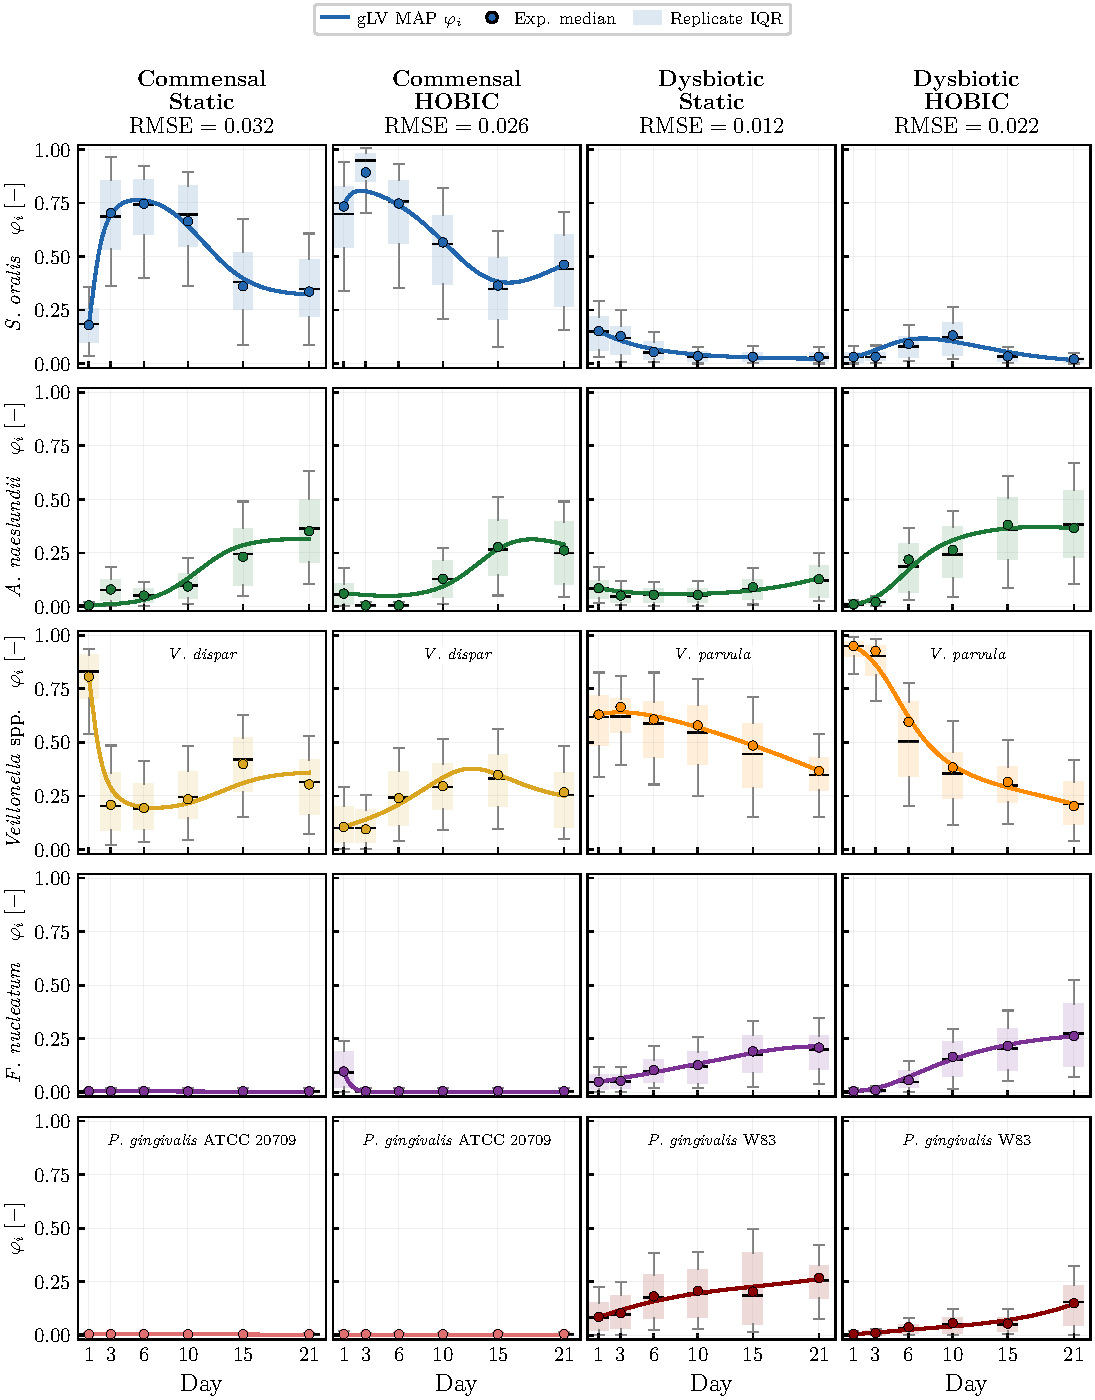
\includegraphics[width=0.80\textwidth]{heine_glv_fit_thesis.pdf}
  \caption[gLV MAP fits across four conditions]{gLV MAP fits of volume fraction
  $\phi_i$. Layout identical to Figure~\ref{fig:heine_fits}: columns CS, CH,
  DS, DH; rows: five species. Solid line: MAP trajectory; circles: experimental
  median; boxes: inter-replicate IQR. \textit{V.~dispar} (commensal) vs.\
  \textit{V.~parvula} (dysbiotic) and \textit{Pg} strain (DSM\,20709 vs.\
  W83) are labelled within each panel. RMSE values are shown in the column
  titles.}
  \label{fig:heine_glv_fit}
\end{figure}

Figure~\ref{fig:heine_fits} shows the Hamilton TMCMC posterior predictive
trajectories. The model reproduces commensal homeostasis (CS:
\textit{So}/\textit{An} growth with \textit{Pg} near zero although it is not
fixed; CH: the \textit{So}-dominated bloom under flow), the
clean pathogen succession of DS, and the
non-linear \textit{Vei}/\textit{Pg} amplification of DH, the late-onset surge
driven by bridge-mediated cross-feeding. Credible bands widen from CS to DH
with the increasing effective dimensionality.

\begin{figure}[p]
  \centering
  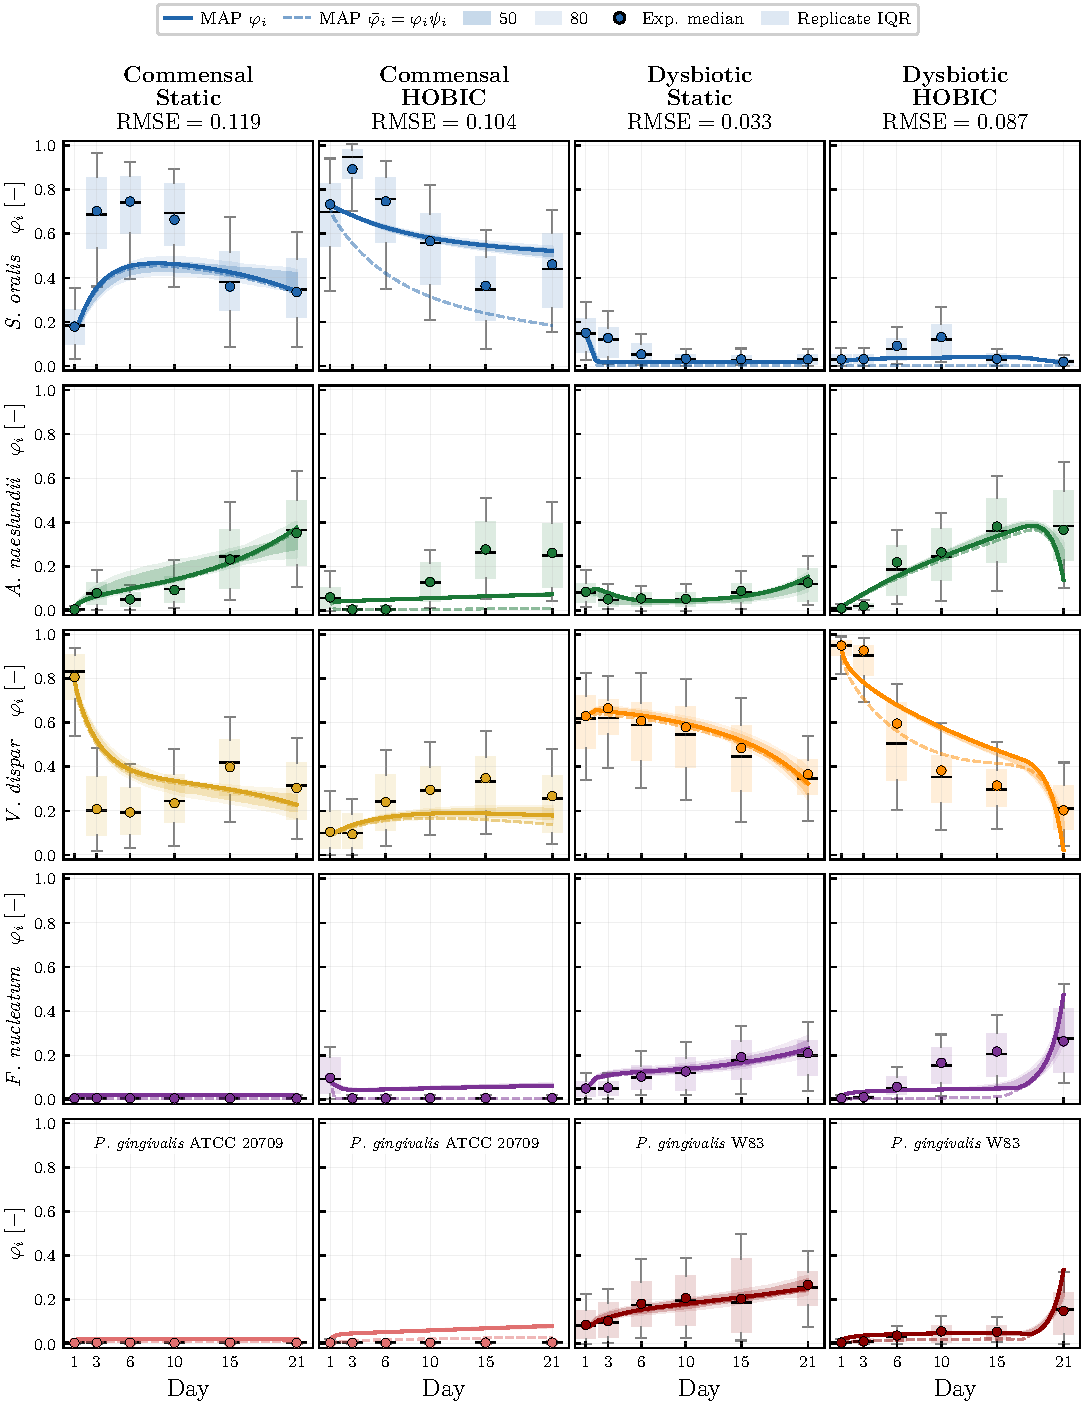
\includegraphics[width=0.82\textwidth]{heine_fits_4cond.pdf}
  \caption[Hamilton TMCMC posterior predictive fits across four conditions]{Hamilton
  TMCMC posterior predictive fits of volume fraction $\phi_i$
  ($N_p=10{,}000$). Columns: CS, CH, DS, DH; rows: five species. Solid: MAP
  $\phi_i$; dashed: living fraction $\bar\phi_i=\phi_i\psi_i$. Bands:
  $50\%$ (dark) / $80\%$ (light) credible intervals from $100$ posterior
  samples. Circles: experimental median ($N=8$); boxes: inter-replicate IQR.
  \textit{Pg} uses different strains by state: avirulent DSM\,20709
  (commensal) vs.\ virulent W83 (dysbiotic).}
  \label{fig:heine_fits}
\end{figure}

\subsection{Inferred interaction matrices and posteriors}
\label{sec:heine_matrices}

The MAP matrices (Figure~\ref{fig:heine_heatmap}) reveal a progressive
reorganisation. In CS/CH the dominant entries are the \textit{So}--\textit{An} and
\textit{So}--\textit{Vei} blocks (the mutualistic early-coloniser core), with the
\textit{Fn} and \textit{Pg} rows near zero. The dysbiotic transition activates
strong positive \textit{Fn}--\textit{Pg} and self-interaction entries:
$\hat a_{55}^{\mathrm{DH}}(\textit{Pg}\,\text{self})=3.43$,
$\hat a_{45}^{\mathrm{DH}}(\textit{Fn}\!\to\!\textit{Pg})=5.63$,
$\hat a_{44}^{\mathrm{DH}}(\textit{Fn}\,\text{self})=4.45$, versus much weaker DS
values ($0.30$, $2.20$, $1.01$) and near-zero CS/CH. The posterior violins
(Figure~\ref{fig:heine_violin}) make the sparsity explicit: the
\textit{Pg}-related entries ($a_{15},a_{25},a_{35},a_{45},a_{55}$) concentrate
sharply at zero in CS/CH without being fixed there, and shift to broad positive
distributions in DS/DH. DS exhibits the narrowest posteriors overall, consistent
with its lowest RMSE.

\begin{figure}[htbp]
  \centering
  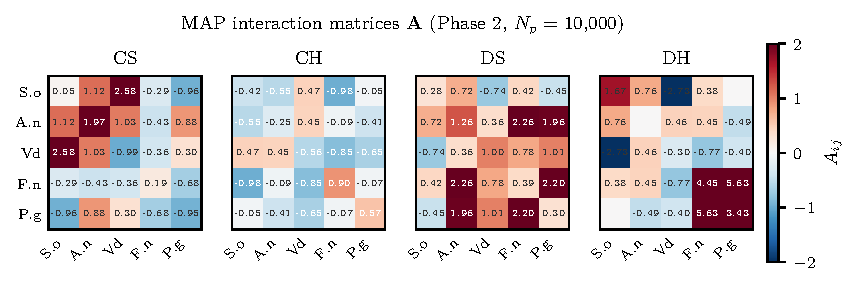
\includegraphics[width=0.80\textwidth]{heine_heatmap_A_4cond.pdf}
  \caption[MAP interaction matrices]{MAP interaction matrices $\mathbf{A}$
  (Phase~2). Red: cooperative ($A_{ij}>0$); blue: competitive ($A_{ij}<0$). In
  CS/CH the \textit{Fn}/\textit{Pg} rows and columns are near zero; these entries
  are estimated, not fixed. The dysbiotic transition activates cooperative
  cross-feeding in the \textit{Fn}--\textit{Pg} block.}
  \label{fig:heine_heatmap}
\end{figure}

The gLV model (no symmetry constraint) yields the same qualitative pattern
with substantially lower RMSE (Table~\ref{tab:glv_hamilton_comparison}).
Figure~\ref{fig:heine_glv_heatmap} shows the corresponding MAP interaction
matrices with annotated entry values. The condition-specific reorganisation is
preserved, while the asymmetry of $\bA$ reveals directed interactions
suppressed by the Hamilton symmetry constraint.

\begin{figure}[htbp]
  \centering
  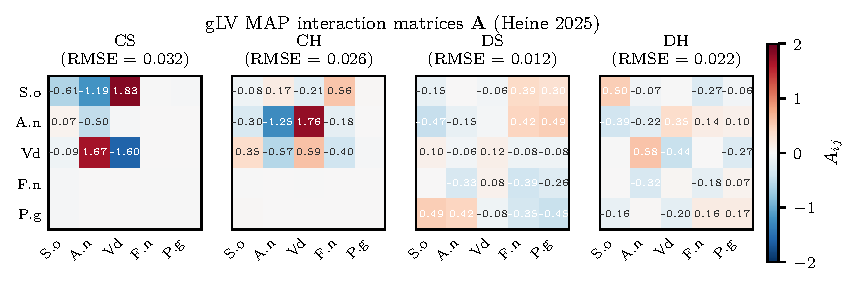
\includegraphics[width=0.80\textwidth]{heine_glv_Amatrix_thesis.pdf}
  \caption[gLV MAP interaction matrices across four conditions]{gLV MAP
  interaction matrices $\mathbf{A}$ (asymmetric). Red: cooperative
  ($A_{ij}>0$); blue: competitive ($A_{ij}<0$). Annotated values indicate
  entries with $|A_{ij}|>0.04$. The CS/CH commensal core
  (\textit{So}--\textit{An}/\textit{Vei}; \textit{Vd} in the figure) and the DS/DH dysbiotic
  \textit{Fn}--\textit{Pg} block are consistent with the Hamilton result
  (Figure~\ref{fig:heine_heatmap}), but the asymmetric entries expose
  directionality absent from the symmetric prior.}
  \label{fig:heine_glv_heatmap}
\end{figure}

Two features emerge from the annotated entries.
% 4 Oct 2026: values re-read from figures/heine_glv_Amatrix_thesis.pdf; the
% earlier text paired a CS and a CH entry and called both CS/CH.
\emph{Magnitude contraction in dysbiosis}: the largest CS/CH entries reach
$|A_{ij}|\!\approx\!1.8$ (CS: $A_{\text{So,Vei}}\!=\!+1.83$, $A_{\text{Vei,An}}\!=\!+1.67$;
CH: $A_{\text{An,Vei}}\!=\!+1.76$), whereas no DS/DH entry exceeds $0.58$, consistent with a tightly coordinated
commensal network versus a weaker but more distributed dysbiotic attractor.
\emph{Directed asymmetry and late-coloniser activation}: in CS, $A_{\text{Vei,An}}\!=\!+1.67$
but $A_{\text{An,Vei}}\!=\!-0.02$, a one-directional benefit invisible to the symmetric model;
in DS/DH the \textit{Pg}-related entries activate (DS: $A_{\text{An,Pg}}\!=\!+0.49$; DH:
$A_{\text{Fn,Pg}}\!=\!+0.07$), consistent with the sign-enrichment analysis of
Section~\ref{sec:heine_signprior}.

\begin{figure}[htbp]
  \centering
  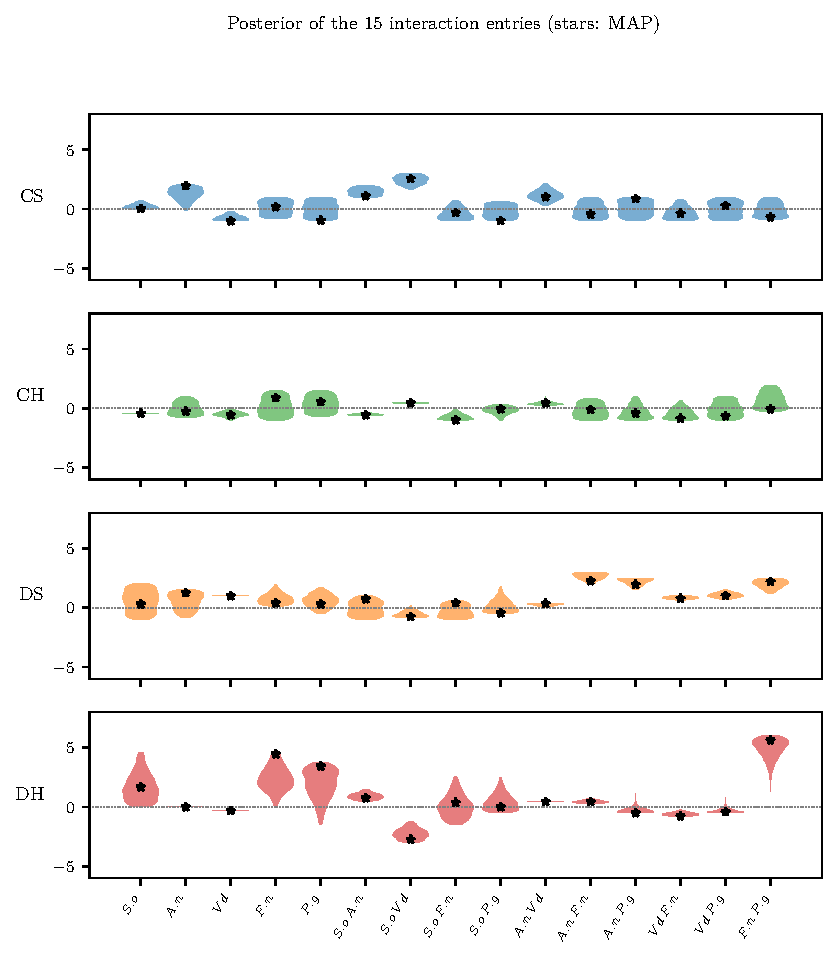
\includegraphics[width=0.82\textwidth]{heine_posterior_violin.pdf}
  \caption[Posterior distributions of the 15 interaction entries]{Posterior
  distributions of the $15$ interaction entries (Phase~2). Stars: MAP. The
  concentration of \textit{Pg}-related entries at zero in CS/CH confirms that
  biological sparsity emerges from the data without a priori locking.}
  \label{fig:heine_violin}
\end{figure}

\subsection{Structural reorganisation across conditions}
\label{sec:heine_reorg}

To quantify the inter-condition differences I compute, for each pair, the
correlation $\rho$ of the vectorised matrices and the relative Frobenius distance
$\Delta_F$ (Table~\ref{tab:heine_pairwise}). Matrices within the same health state
share a backbone ($\rho_{\text{CH--CS}}=+0.26$, $\rho_{\text{DH--DS}}=+0.40$),
whereas three of the four cross-state pairs anticorrelate ($\rho_{\text{DH--CS}}=-0.49$),
and all cross-state pairs have large distances ($\Delta_F\geq1.01$). A UMAP
embedding~\cite{McInnes2018UMAP} (cf.\ t-SNE~\cite{VanDerMaaten2008tSNE}) of the full posterior
(Figure~\ref{fig:heine_umap}) confirms four well-separated clusters with no
overlap. The transition from health to disease thus changes the sign pattern of
the interaction network (Table~\ref{tab:heine_rewiring}).

\begin{table}[htbp]
  \centering\small
  \begin{tabular}{@{}cc|ccc@{}}
    \toprule
    \textbf{C1} & \textbf{C2} & $\rho$ & $\Delta_F$ & $d_{15\mathrm{D}}$\\
    \midrule
    CH & CS & $+0.26$ & $1.06$ & $\mathbf{3.38}$\\
    DH & DS & $\mathbf{+0.40}$ & $\mathbf{0.88}$ & $5.86$\\
    CH & DH & $+0.24$ & $1.01$ & $6.33$\\
    CH & DS & $-0.27$ & $1.27$ & $4.88$\\
    DH & CS & $\mathbf{-0.49}$ & $1.28$ & $\mathbf{7.77}$\\
    CS & DS & $-0.27$ & $\mathbf{1.36}$ & $5.88$\\
    \bottomrule
  \end{tabular}
  \caption[Pairwise comparison of MAP matrices]{Pairwise comparison of MAP
  matrices. $\rho$: correlation of $\mathrm{vec}(\mathbf{A})$; $\Delta_F$: relative
  Frobenius distance; $d_{15\mathrm{D}}$: posterior-centroid distance in 15D.}
  \label{tab:heine_pairwise}
\end{table}

\begin{figure}[htbp]
  \centering
  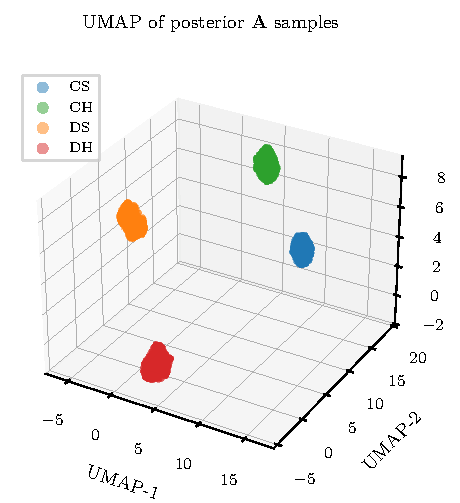
\includegraphics[width=0.56\textwidth]{heine_umap_A_3d.pdf}
  \caption[UMAP embedding of posterior A-matrix samples]{UMAP 3D embedding of the
  posterior A-matrix samples ($N_p=10{,}000$). The four conditions form
  well-separated clusters; centroid distances mirror the $d_{15\mathrm{D}}$ ordering
  (CS--CH closest, CS--DH most distant).}
  \label{fig:heine_umap}
\end{figure}

Figure~\ref{fig:heine_umap_comparison} overlays the gLV MAP solutions on the same
UMAP embedding (fitted on the Hamilton posterior; gLV projected via
$\tilde{A}_{ij}=(A_{ij}+A_{ji})/2$). Hamilton MAP stars ($\bigstar$) fall within their
posterior clouds in all four conditions; gLV MAP crosses ($\times$) deviate substantially
for CS and DH, migrating toward the CH region and the embedding centre respectively.
The lower gLV RMSE shows that the displacement reflects asymmetry unlocking regions of interaction space geometrically
inaccessible under the $A_{ij}=A_{ji}$ constraint.

\begin{figure}[htbp]
  \centering
  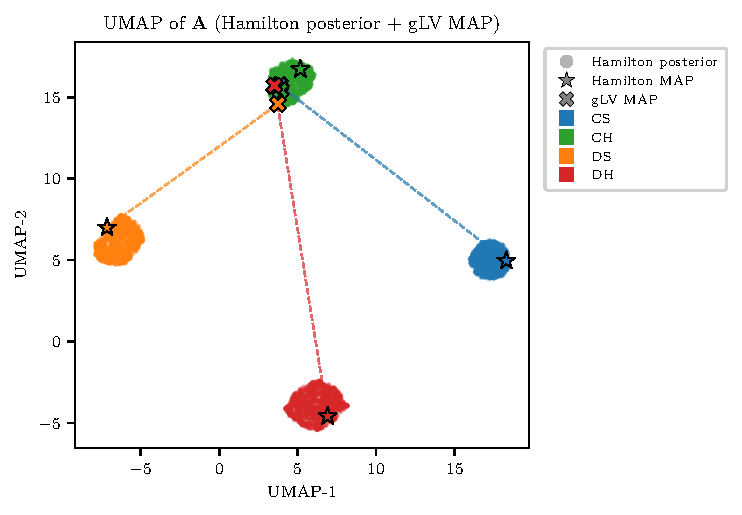
\includegraphics[width=0.64\textwidth]{heine_umap_comparison.pdf}
  \caption[UMAP comparison: Hamilton posterior and gLV MAP]{UMAP of the
  Hamilton posterior A-matrix samples (a subsample of $1{,}200$ per condition from
  the $N_p=10{,}000$ posterior; coloured clouds). Stars ($\bigstar$): Hamilton MAP; crosses ($\mathbf{\times}$):
  gLV MAP, projected via $\tilde{A}_{ij}=(A_{ij}+A_{ji})/2$. Dashed lines
  connect Hamilton MAP to gLV MAP of the same condition. Legend at right.
  CS and DH gLV MAP solutions are displaced well outside their Hamilton
  posterior clouds, indicating that asymmetry unlocks qualitatively different
  regions of interaction space.}
  \label{fig:heine_umap_comparison}
\end{figure}

Cross-condition \emph{transfer} sharpens the point (Table~\ref{tab:heine_transfer}):
evaluating each MAP on every other condition's data, the within-state commensal
transfer CS$\to$CH (RMSE $0.098$) is better than the CH self-prediction ($0.104$),
which points to a shared commensal backbone across cultivation modes, whereas
cross-state transfers (DS$\to$CS $0.384$, CS$\to$DH $0.198$) degrade sharply.

\begin{table}[htbp]
  \centering\small
  \begin{tabular}{@{}lcccc@{}}
    \toprule
    Source $\backslash$ Target & CS & CH & DS & DH \\
    \midrule
    CS & \textbf{0.119} & 0.098 & 0.261 & 0.198 \\
    CH & 0.257 & \textbf{0.104} & 0.100 & 0.159 \\
    DS & 0.384 & 0.259 & \textbf{0.033} & 0.255 \\
    DH & 0.342 & 0.212 & 0.289 & \textbf{0.087} \\
    \bottomrule
  \end{tabular}
  \caption[Cross-condition prediction RMSE]{Cross-condition prediction RMSE.
  Diagonal (bold): self-prediction. CS$\to$CH ($0.098$) outperforms CH
  self-prediction ($0.104$), confirming a shared commensal backbone.}
  \label{tab:heine_transfer}
\end{table}

\paragraph{Effective dimensionality.} With $r_i=\sigma_{\mathrm{post},i}/\Delta_{\mathrm{prior}}$
($\Delta_{\mathrm{prior}}=6$), all $15$ parameters satisfy $r_i<0.43$ in every
condition (DS tightest, mean $r=0.07$), and even the commensal \textit{Pg} entries
reach $r_i\leq0.10$: the data constrain them to near zero. The full $15$-parameter model is therefore not over-parametrised
(the identifiability diagnostic of Section~\ref{sec:theory_tmcmc}).

\subsection{Edge rewiring between health states}
\label{sec:heine_rewiring}

The structural reorganisation of Section~\ref{sec:heine_reorg} can be localised to
individual edges by classifying each pair as facilitative or competitive
from the full posterior (the facilitation probability $P_{\mathrm{fac}}$ is the
posterior mass with $A_{ij}>0$). A handful of edges flip sign with near-certainty
between the commensal and dysbiotic states (Table~\ref{tab:heine_rewiring}). The
\textit{So}--\textit{Vei} lactate axis, the metabolic core
of commensal health, reverses from strong mutual facilitation
($P_{\mathrm{fac}}\!\approx\!1.0$) to competition ($P_{\mathrm{fac}}\!<\!0.05$),
while \textit{F.~nucleatum} acquires facilitation from \textit{An} and
\textit{Vei} ($P_{\mathrm{fac}}$ rising from $0.09$--$0.23$ to $0.77$--$0.97$).
Consistently, the net outgoing effect of \textit{P.~gingivalis} is most negative in
dysbiotic-HOBIC ($\overline{\Delta}_{\textit{Pg}}^{\,\mathrm{DH}}=-0.14$,
$P_{\mathrm{fac}}=0.27$): in the surge regime \textit{Pg} is a net competitor
that consumes the shared niche rather than feeding it.

\begin{table}[htbp]
  \centering\small
  \begin{tabular}{@{}llcc@{}}
    \toprule
    Edge & Commensal $\to$ Dysbiotic & $P_{\mathrm{fac}}^{\mathrm{comm}}$ & $P_{\mathrm{fac}}^{\mathrm{dys}}$\\
    \midrule
    \textit{So}--\textit{Vei} & facilitation $\to$ competition & $1.00$ & $0.00$--$0.03$\\
    \textit{An}--\textit{Fn}  & competition $\to$ facilitation & $0.23$ & $0.97$\\
    \textit{Vei}--\textit{Fn} & competition $\to$ facilitation & $0.09$ & $0.77$\\
    \bottomrule
  \end{tabular}
  \caption[Posterior edge rewiring between health states]{Edges that flip sign with
  near-certainty between commensal and dysbiotic states (posterior facilitation
  probability $P_{\mathrm{fac}}$, from the $10{,}000$-particle posterior). $\mathbf A$
  is symmetric, so each edge is undirected; where two values are given they span the
  dysbiotic estimates. The
  commensal \textit{So}--\textit{Vei} lactate mutualism reverses to competition; the
  bridging organism \textit{F.~nucleatum} gains facilitation.}
  \label{tab:heine_rewiring}
\end{table}

%==============================================================================
\section{Independent Validation}
\label{sec:heine_validation}
%==============================================================================

The Phase-2 MAP parameters are validated against measurements that never entered
the calibration.

\paragraph{pH prediction (LOO-$R^2=0.92$; independent $R^2=0.78$).}
A five-predictor linear pH model, selected by leave-one-out CV on $N=90$ HOBIC
time points,
\begin{equation}
  \mathrm{pH}(t) = 6.10 + 0.16\,\phi_{\textit{So}} + 0.55\,\phi_{\textit{An}}
    + 0.30\,\phi_{\textit{Vei}} + 1.22\,\phi_{\textit{Fn}} + 1.88\,\phi_{\textit{Pg}},
  \label{eq:heine_ph}
\end{equation}
has its coefficients fixed from \emph{experimental} fractions alone
(LOO-$R^2=0.920$). To test the \emph{inferred} $\mathbf{A}$, $500$ Phase-2
posterior samples are integrated forward from Day-1 fractions and the fixed
coefficients applied to the ODE-predicted fractions; no pH data enter
the TMCMC. This gives an independent $R^2=0.778$ (RMSE $0.126$\,pH units)
against the held-out HOBIC pH series (Figure~\ref{fig:heine_ph}), confirming that
$\mathbf{A}$ captures the community drivers of pH. The species--pH correlations are
mechanistically coherent: \textit{Fn} ($r=+0.93$) and \textit{Pg} ($r=+0.93$)
dominate alkalinisation (gingipain-mediated arginine/lysine catabolism releasing
ammonia), while \textit{So} acidifies ($r=-0.68$) via lactate.

\begin{figure}[htbp]
  \centering
  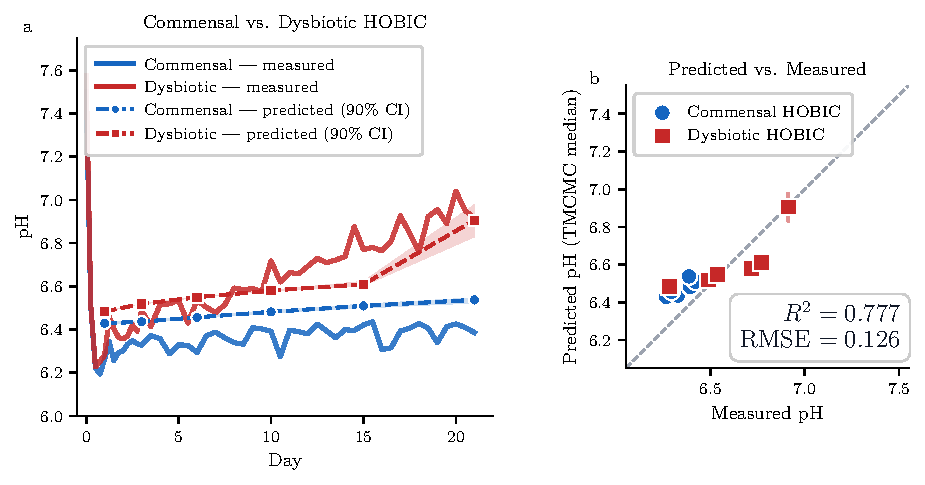
\includegraphics[width=0.80\textwidth]{heine_ph_validation.pdf}
  \caption[Independent pH validation]{Independent pH validation. \textbf{(a)}
  Measured HOBIC pH (solid) vs.\ TMCMC posterior predictions (dashed, markers) with
  $90\%$ credible bands, commensal (blue) and dysbiotic (red). \textbf{(b)}
  Predicted vs.\ measured pH at six time points. Regression coefficients were
  fitted from species fractions only (LOO-CV, $N=90$); pH was not used in
  calibration. $R^2=0.778$, RMSE $0.126$\,pH units.}
  \label{fig:heine_ph}
\end{figure}

\paragraph{Further checks.} The predicted DH \textit{Pg} trajectory correlates
with the measured gingipain profile ($r=0.90$), both showing delayed Day-15--21
onset. The signs of the posterior are metabolically plausible: the \textit{So}--\textit{Vei}
lactate axis is facilitative in the commensal states and competitive in the
dysbiotic states, and the \textit{Fn} edges gain facilitation in the dysbiotic
states (Table~\ref{tab:heine_rewiring}).
Section~\ref{sec:heine_signprior} uses such metabolic signs as a prior for
in-vivo data.

%==============================================================================
\section{Discussion}
\label{sec:heine_discussion}
%==============================================================================

\paragraph{Biological interpretation.} The inferred matrices give a quantitative
account of the commensal-to-dysbiotic transition. The healthy state rests on a
\textit{So}--\textit{An} co-aggregation and \textit{So}--\textit{Vei} lactate core;
dysbiosis activates cooperative \textit{Vei}$\to$\textit{Pg} and
\textit{Fn}$\to$\textit{Pg} pathways. That structural similarity is preserved
within health states ($\rho_{\text{within}}>0$) but lost across them
($\rho_{\text{cross}}<0$ for three of the four cross-state pairs) shows the transition to be a network reorganisation
rather than a magnitude shift, and the full-discovery posterior recovers commensal
sparsity as an emergent property.

\paragraph{A falsifiable prediction.} Because the terminal \textit{Pg} surge is
gated by the cooperative \textit{Fn}$\to$\textit{Pg} coefficient, which is
indistinguishable from zero in both commensal states but rises to
$\hat a_{45}^{\mathrm{DH}}=5.63$ (posterior mean $+4.86$, $95\%$ CI
$[+3.03,+5.95]$) under dysbiotic flow, the model predicts that
\emph{attenuating this single interaction}, e.g.\ by omitting
\textit{F.~nucleatum} from the consortium, should suppress the terminal \textit{Pg}
bloom and drive the DH trajectory toward a commensal-like, \textit{Pg}-low steady
state. This is a direct leave-one-species-out co-culture test that would
discriminate the network hypothesis from a \textit{Pg}-intrinsic growth
explanation, and it recapitulates the established bridging role of
\textit{F.~nucleatum}~\cite{Kolenbrander2006FnBridge, Signat2011Fn}.

\paragraph{Fix-$\psi$ approximation and Phase~2.} Figure~\ref{fig:heine_phase}
compares the Phase-1 and Phase-2 MAPs parameter by parameter. In commensal
conditions they agree closely ($r=0.83$--$0.90$): the $\psi$--$\mathbf{A}$ coupling
is weak and fix-$\psi$ is a good approximation. In dysbiotic conditions they
diverge ($r=0.23$ for DS, $0.62$ for DH), with the largest shifts in
\textit{Pg}-related entries, where viability dynamics are most active.
This condition-dependent consistency validates the two-phase design: Phase~1 is a
reliable starting point, and Phase~2 corrections matter where $\psi$ couples
non-negligibly to $\mathbf{A}$. The viability predictions themselves remain poor
(RMSE $0.11$--$0.39$); the $\psi$ channel functions as a soft constraint that
breaks the $\psi$--$\mathbf{A}$ degeneracy rather than as a predictive model of
membrane integrity.

\begin{figure}[htbp]
  \centering
  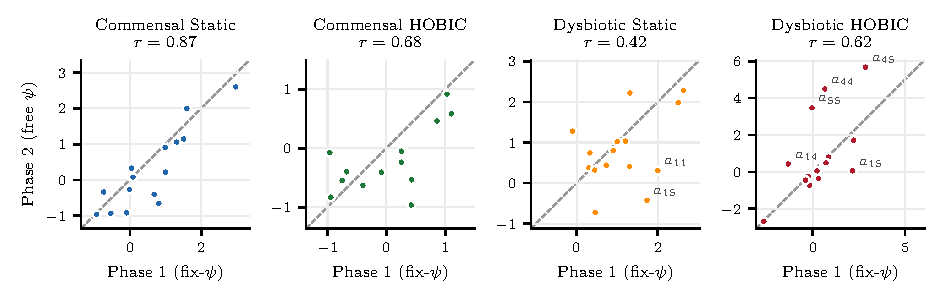
\includegraphics[width=0.80\textwidth]{heine_phase1_vs_phase2.pdf}
  \caption[Phase~1 vs.\ Phase~2 MAP estimates]{Phase~1 (fix-$\psi$) vs.\ Phase~2
  (free $\psi$) MAP estimates; each point is one of the $15$ parameters, dashed
  line is identity. Commensal conditions agree strongly ($r\geq0.83$); dysbiotic
  conditions shift systematically in \textit{Pg}-related parameters, confirming the
  necessity of Phase~2.}
  \label{fig:heine_phase}
\end{figure}

\paragraph{Model evidence and computation.} The log-evidence $\ln\hat Z$~\cite{Kass1995Bayes}
(Table~\ref{tab:heine_rmse}) is higher for the commensal conditions in Phase~1 under the same
$15$-parameter prior, because the posterior concentrates pathogen entries near
zero and so reduces the Occam factor, a model-based signature of ecological
complexity. Methodologically, the $147\times$ GPU speedup makes
$10{,}000$-particle posteriors routine and is what renders the full-discovery,
no-locking strategy tractable in $15$ dimensions. These in-vitro interaction
matrices, and the validation that they predict held-out chemistry, calibrate the
point model that Chapter~\ref{ch:ansys} brings into space.

\paragraph{Limitations and the symmetry approximation.}
Three limitations bound interpretation of the in-vitro matrices. First, the
Hamilton symmetry constraint $A_{ij}=A_{ji}$ excludes directed
contact-dependent adhesion and toxin delivery by construction. Second, the
five-species consortium is a curated subset; unmeasured community members
could absorb metabolites that shift apparent cross-feeding signs. Third,
the Phase-1 posteriors are conditioned on the measured viability, and Phase~2
treats $\psi$ only as a soft constraint; a fully
joint $(\mathbf{A},\psi)$ inference would propagate additional uncertainty
into the interaction estimates, particularly in dysbiotic conditions where
the Phase-2 correction is largest. These approximations are consistent with
the in-vitro setting and motivate the in-vivo cross-validation of
Section~\ref{sec:heine_signprior}, where the symmetry constraint is
re-examined against a ten-patient longitudinal dataset.

%==============================================================================
\section{From In-Vitro to In-Vivo Data: a Metabolic Sign Prior}
\label{sec:heine_signprior}
%==============================================================================
% Condensed 3 Oct 2026 from the former chapter 4 (chapters/ch4_dieckow.tex,
% kept in the tree for its full text and figures). Internship work.

The calibration above rests on rich in-vitro data: five species, six time points,
four controlled conditions. Clinical data are much sparser. This section shows,
in condensed form, how the same type of model can still be identified there when
the signs of the interactions are fixed beforehand from metabolic models. The
work was done during an internship at NIFE together with S.\,P.\ Szafra\'{n}ski
and is summarised here because it completes the calibration side of the
thesis; the full analysis is available as an internal report.

\paragraph{Data.} Dieckow et al.~\cite{dieckow2024structure} characterised
early biofilm formation on implant abutments in $12$ patients. The analysis
uses $10$ of them, each sampled at three weekly time points. The
16S~rRNA amplicon reads were aggregated into $10$ class-level guilds and
normalised to the simplex, $\sum_i\phi_i=1$. With $10$ guilds and three time
points, the first of which is the initial condition, there are $20$ observations per patient against up to $55$ entries of a
symmetric interaction matrix, so the inverse problem cannot be solved without
additional information.

\paragraph{Sign prior.} The prior of Section~\ref{sec:theory_fba} is assembled
in three layers: experimentally documented production and use of metabolites
from eHOMD~\cite{Escapa2018eHOMD} and Szafra\'{n}ski et
al.~\cite{Szafranski2025} ($34$ constrained guild pairs); parsimonious FBA of
one AGORA2 model per guild~\cite{Heinken2023AGORA2} ($35$ pairs); and
community FBA with MICOM~\cite{Diener2020MICOM} ($72$ pairs). The directed
signals are symmetrised for the symmetric model, and the penalty acts only on
coefficients of the wrong sign.

\paragraph{Model and test.} The replicator form of
Section~\ref{sec:theory_replicator} is fitted with one interaction matrix
$\bA$ shared by all patients and a growth vector $\bb^{(p)}$ per patient. It is
tested by leave-one-patient-out cross-validation: $\bA$ is fitted on nine
patients and frozen, the held-out patient's $\bb^{(p)}$ is fitted from the
first week only, and the second and third weeks are predicted.
Table~\ref{tab:heine_signprior} lists the prediction errors.

\begin{table}[htbp]
  \centering\small
  \begin{tabular}{@{}llcc@{}}
    \toprule
    model & prior & sign agreement & LOO-RMSE\\
    \midrule
    replicator, symmetric $\bA$ & none            & --        & $0.0595$\\
    replicator, symmetric $\bA$ & eHOMD + pFBA    & $94\%$    & $0.0516$\\
    replicator, symmetric $\bA$ & + MICOM         & $100\%$   & $0.0502$\\
    gLV, asymmetric             & none            & --        & $0.0588$\\
    gLV, asymmetric             & eHOMD + pFBA    & $97\%$    & $0.0490$\\
    Bayesian gLV (MDSINE2~\cite{Gibson2021MDSINE2}) & sparsity & -- & $0.0552$\\
    \bottomrule
  \end{tabular}
  \caption[Leave-one-patient-out prediction with a sign prior]{Leave-one-patient-out
    prediction of the in-vivo guild compositions ($10$ patients of Dieckow et al.).
    Sign agreement: share of the constrained pairs whose fitted sign matches the
    prior. The persistence null model has a Bray--Curtis dissimilarity of
    $0.281$; the best model reaches $0.147$.}
  \label{tab:heine_signprior}
\end{table}

\paragraph{Results.}
\begin{itemize}
  \item The sign prior improves the symmetric model step by step, from
        $0.0595$ without prior to $0.0502$ with all three layers. The
        asymmetric gLV with the first two layers is slightly better
        ($0.0490$); its directed coefficients add freedom that the symmetric
        model does not have. The Bayesian gLV collapses to $\bA\approx0$ with
        three time points.
  \item Only the sign carries over from the metabolic models. A prior that
        ties $A_{ij}$ to the magnitude of the predicted fluxes recovers the
        correct sign for only $4$ to $11$ of $70$ pairs. Fitted without any
        prior, the symmetric model still recovers $11$ of the $14$
        cross-feeding signs predicted by AGORA2 ($78.6\,\%$, against $37.7\,\%$
        under a permutation null, $p=4\times10^{-4}$); the asymmetric gLV
        shows no such agreement ($p=0.96$).
  \item On $127$ independent peri-implant samples of Joshi et
        al.~\cite{joshi2025}, a dysbiosis ratio of the guilds ordered by the
        model separates peri-implantitis from health and mucositis
        (Kruskal--Wallis $p<10^{-4}$; Spearman $\rho=0.46$ with severity).
\end{itemize}

\paragraph{Limits.} With $10$ patients the gain of the community-FBA layer over
the first two is only marginally significant ($p\approx0.07$). The symmetric
matrix cannot represent directed effects, which is where the asymmetric gLV
gains its edge. For the rest of this thesis the result that matters is a
narrower one: the signs of the interaction matrix are the part of the model
that is supported by independent evidence, in vitro and in vivo.

% Structure of 3 Oct 2026 (thesis/README.md): the old ch4 (Dieckow, internship
% work) is to be condensed into one section of ch3; the old ch5 (spatial PDE,
% FISH, Abaqus-era stresses) is out of scope. Both stay in chapters/ until
% their material has been moved.
% \chapter{Metabolic-Prior Replicator Dynamics for In-Vivo Oral Microbiome}
\label{ch:dieckow}

Where Chapter~\ref{ch:heine} identified interaction matrices from a defined
\emph{in-vitro} consortium, this chapter turns to the harder \emph{in-vivo}
regime: longitudinal 16S~rRNA data from a clinical cohort, where the community is
ten guilds wide, the time series only three points deep, and the interactions must
be regularised to be identifiable at all. The central idea of the thesis appears
here in full --- the off-diagonal \emph{sign} of the interaction matrix is
constrained from metabolic evidence (a flux-balance-derived sign prior), while its
magnitude is left to the data --- and is shown to be the property that actually
generalises out of sample.

\medskip\noindent\textit{This chapter is based on the internal analysis document:}
Nishioka K., Szafra\'{n}ski S.P., ``Metabolic-Prior Replicator Dynamics Predict
Oral Microbiome Community Composition under Leave-One-Out Cross-Validation''
(NIFE/IKM collaboration).

%==============================================================================
\section{Dataset and Guild Taxonomy}
\label{sec:dieckow_data}
%==============================================================================

We use the 16S~rRNA amplicon data of Dieckow et al.~\cite{dieckow2024}, a
prospective study of subgingival plaque on titanium implant abutments from
$10$ patients sampled at three weekly time points (W1, W2, W3). Reads were
processed by a standard amplicon pipeline --- ASV inference with DADA2~\cite{Callahan2016DADA2},
taxonomic classification against SILVA~\cite{Quast2013SILVA, Bokulich2018FeatureClassifier, Robeson2021RESCRIPt} within
QIIME2~\cite{Bolyen2019QIIME2} (VSEARCH~\cite{Rognes2016VSEARCH}), orchestrated by Nextflow~\cite{DiTommaso2017Nextflow}, referenced to the
human oral microbiome taxonomy~\cite{Dewhirst2010HOMD} --- and the resulting ASVs are
aggregated to the canonical $10$ class-level guilds used throughout this thesis
(Table~\ref{tab:dieckow_guilds}; the ordering is the project-wide standard against
which all abundance arrays are indexed), and each compositional vector is
$\ell^1$-normalised to the unit simplex, $\sum_i\phi_i=1$ --- relative-abundance data
being inherently compositional~\cite{Aitchison1982Compositional, Aitchison1986Compositional, PawlowskyGlahn2015Compositional, Gloor2017Microbiome}. Following
Dieckow et al., a Gaussian-mixture clustering of the W1 compositions splits the
cohort into two \emph{community types}: CT1 ($5$ patients), enriched in early
commensal colonisers (Actinobacteria, Bacilli, Betaproteobacteria), and CT2
($5$ patients), enriched in Fusobacteriia and Bacteroidia. With only
$K\times(T-1)=20$ observations per patient against an interaction matrix of up to
$K(K{+}1)/2=55$ entries, regularisation is not optional.

\begin{table}[htbp]
  \centering\small
  \begin{tabular}{@{}cll@{}}
    \toprule
    \textbf{Index} & \textbf{Guild} & \textbf{SILVA 138.1 class / order}\\
    \midrule
    0 & Actinobacteria      & Actinobacteria, Actinomycetia\\
    1 & Bacilli             & Bacilli\\
    2 & Bacteroidia         & Bacteroidia\\
    3 & Betaproteobacteria  & Betaproteobacteria\\
    4 & Clostridia          & Clostridia, Erysipelotrichia\\
    5 & Coriobacteriia      & Coriobacteriia\\
    6 & Fusobacteriia       & Fusobacteriia, Fusobacteriales\\
    7 & Gammaproteobacteria & Gammaproteobacteria\\
    8 & Negativicutes       & Negativicutes, Selenomonadales, Veillonellales\\
    9 & Other               & All remaining classes\\
    \bottomrule
  \end{tabular}
  \caption[Ten class-level guilds]{The ten class-level guilds (canonical
  ordering). The same guild definitions are used across all datasets in this
  thesis so that abundance arrays and interaction matrices are directly comparable.}
  \label{tab:dieckow_guilds}
\end{table}

%==============================================================================
\section{Three-Layer Metabolic Sign Prior}
\label{sec:dieckow_prior}
%==============================================================================

The sign prior is the thesis's central regulariser. It encodes a single biological
rule --- \emph{if guild $j$ produces a metabolite consumed by guild $i$, then
$A_{ij}>0$ regardless of magnitude} --- and is assembled in three layers of
increasing mechanistic resolution (building on the FBA machinery of
Section~\ref{sec:theory_fba}; Figure~\ref{fig:dieckow_pipeline}).

\paragraph{L1 --- eHOMD / Szafra\'{n}ski experimental flows.} Experimentally
confirmed produces/uses/inhibits relationships between guild-level taxa and oral
metabolites, curated from the expanded Human Oral Microbiome Database
(eHOMD)~\cite{Escapa2018eHOMD} and the Szafra\'{n}ski et al.\ supplement~\cite{Szafranski2025}. Cross-feeding
contributes $+w_{L1}$, competition/inhibition $-w_{L1}$ ($w_{L1}=2.0$ for direct
experimental evidence, $1.5$ literature-supported). L1 alone constrains $34$ guild
pairs.

\paragraph{L2 --- AGORA2 pFBA.} Parsimonious FBA on one representative genome-scale
metabolic model per guild (AGORA2 v2.01~\cite{Heinken2023AGORA2}) under a standardised
oral-fluid medium. pFBA minimises total flux at the optimal growth rate, giving
sparse, sign-robust secretion/uptake patterns; the four strictly anaerobic guilds
have their O$_2$ exchange shut off, and inorganic ions/gases are excluded as
non-syntrophic. Adding L2 ($w_{L2}=1.0$) extends the constrained set only from $34$
to $35$ pairs --- L1 already captures the dominant experimentally-known
cross-feeding.

\paragraph{L3 --- MICOM community FBA.} Single-species pFBA misses the resource
competition and cross-feeding that emerge only when all guilds share one medium.
MICOM~\cite{Diener2020MICOM} solves a community FBA over all $10$ guild models under the
cooperative trade-off
\begin{equation}
  \text{maximise}\;\min_i\!\Bigl(\tfrac{\mu_i}{\mu_i^{\max}}\Bigr)
  \quad\text{s.t.}\quad \textstyle\sum_i\mu_i\geq\tau\sum_i\mu_i^{\max},
  \qquad \tau=0.5,
  \label{eq:dieckow_micom}
\end{equation}
from whose flux solution flux-weighted cross-feeding ($+$) and diffusible-toxin
($-$, e.g.\ H$_2$O$_2$/H$_2$S) signals are extracted. L3 adds $37$ pairs (total
$72$) and the result is robust to $\tau\in\{0.3,0.4,0.5\}$ ($\Delta$RMSE$<0.001$).

\paragraph{Net flow and penalty.} Because the Hamilton matrix is symmetric, the
directed signals are symmetrised, $F_{ij}=\tfrac12(\mathrm{net}[i,j]+\mathrm{net}[j,i])$,
giving prior sign $s_{ij}=\sgn(F_{ij})$ with stiffness $|F_{ij}|$; the asymmetric
gLV uses the directed matrix without symmetrisation. The prior enters the loss as a
half-normal (hinge-squared) penalty that is \emph{zero for correct-sign $A_{ij}$}
and quadratic only for violations,
\begin{equation}
  \calP(\bA;\bF)
  = \sum_{F_{ij}\neq0}\frac{|F_{ij}|}{2\sigma^2}
    \bigl[\max(0,\,-\sgn(F_{ij})\,A_{ij})\bigr]^2,
  \qquad \sigma=0.15,
  \label{eq:dieckow_penalty}
\end{equation}
so it constrains \emph{sign, never magnitude} --- a deliberate choice justified
post hoc in Section~\ref{sec:dieckow_results} (FBA flux units are not ecological
interaction units). The full objective adds a data term and a mild ridge,
$\calL=\mathrm{RMSE}(\hat\bphi,\bphi)+\calP(\bA;\bF)+\lambda\|\bA\|_F^2$
($\lambda=10^{-4}$), minimised by L-BFGS-B with JAX autodiff gradients.

%==============================================================================
\section{Models and Cross-Validation}
\label{sec:dieckow_models}
%==============================================================================

The primary model is the Hamilton replicator (symmetric $\bA$, shared across
patients; patient-specific growth $\bb^{(p)}$) of Section~\ref{sec:theory_replicator},
$\dot\phi_i=\phi_i(f_i(\bphi)-\bar f)$ with $f_i=b_i+\sum_jA_{ij}\phi_j$ and
$A_{ii}\leq0$. For comparison we fit (i) an \emph{asymmetric} gLV (integrated by an explicit Runge--Kutta scheme~\cite{Dormand1980RK45}; no symmetry, no
sign prior unless stated; double the off-diagonal freedom, a ceiling on
expressiveness), (ii) a Hamilton Normal-Species-Pool (NSP) variant optimised by a
three-step implicit-function-theorem scheme, and (iii) MDSINE2~\cite{Bucci2016MDSINE, Gibson2021MDSINE2}, a
fully Bayesian gLV, as a sparsity-induction baseline.

Generalisation is measured by leave-one-patient-out (LOO) cross-validation: for
each held-out patient, $\bA$ and the training $\bb^{(q)}$ are fit on the other
$9$; $\bA$ is frozen; the held-out $\bb^{(p)}$ is fit from W1 only; W2--W3 are
predicted and scored by RMSE and Bray--Curtis (BC) dissimilarity~\cite{Bray1957BrayCurtis, Whittaker1960Diversity}.

%==============================================================================
\section{Results}
\label{sec:dieckow_results}
%==============================================================================

\subsection{Interaction matrix and sign recovery}
\label{sec:dieckow_A}

The fitted matrix (Figure~\ref{fig:dieckow_A}) has all-negative diagonals
(self-limitation) and its dominant facilitations are among early commensal
colonisers --- Actinobacteria--Bacilli ($A_{01}=+1.61$),
Bacilli--Betaproteobacteria ($A_{13}=+1.83$), Actinobacteria--Betaproteobacteria
($A_{03}=+1.67$) --- consistent with documented co-aggregation, while Fusobacteriia
interacts net-negatively with early colonisers (its late-bridging role). The full
L1+L2+L3 prior achieves $70/70$ ($100\%$) sign agreement with the fitted $\bA$ at
$W^*{=}1.0$ --- the lowest weight that achieves full consistency and simultaneously
minimises training RMSE --- and MICOM's $72$ constrained pairs reach $72/72$.

\begin{figure}[htbp]
  \centering
  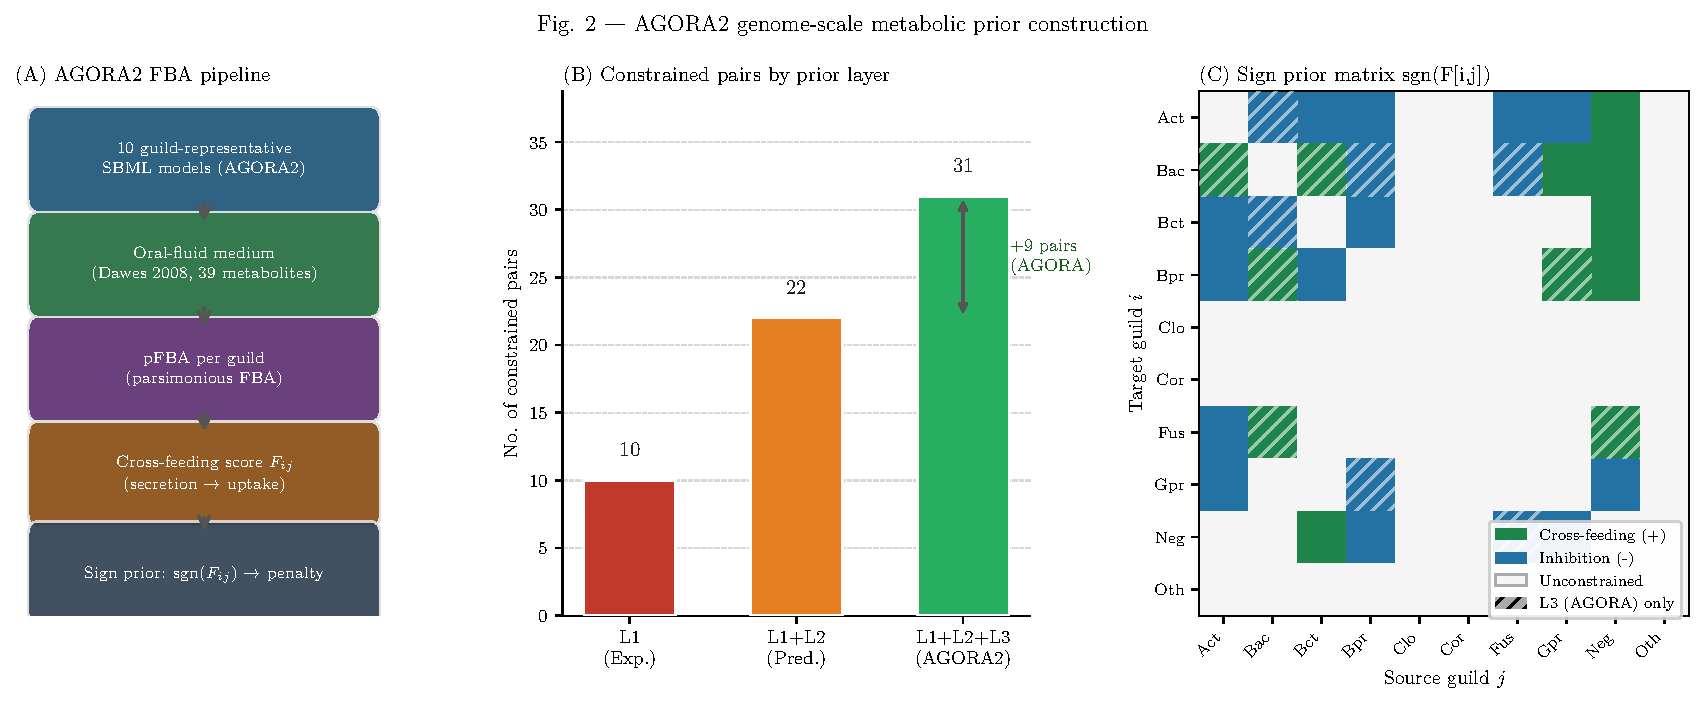
\includegraphics[width=0.80\textwidth]{dieckow_sign_pipeline.pdf}
  \caption[Three-layer sign-prior construction]{Construction of the metabolic sign
  prior. Oral-fluid medium $\to$ per-guild pFBA $\to$ community MICOM $\to$ signed
  net-flow matrix $F_{ij}$. Constrained pairs by layer: L1 ($34$), L1+L2 ($35$),
  L1+L2+L3 ($72$).}
  \label{fig:dieckow_pipeline}
\end{figure}

\begin{figure}[htbp]
  \centering
  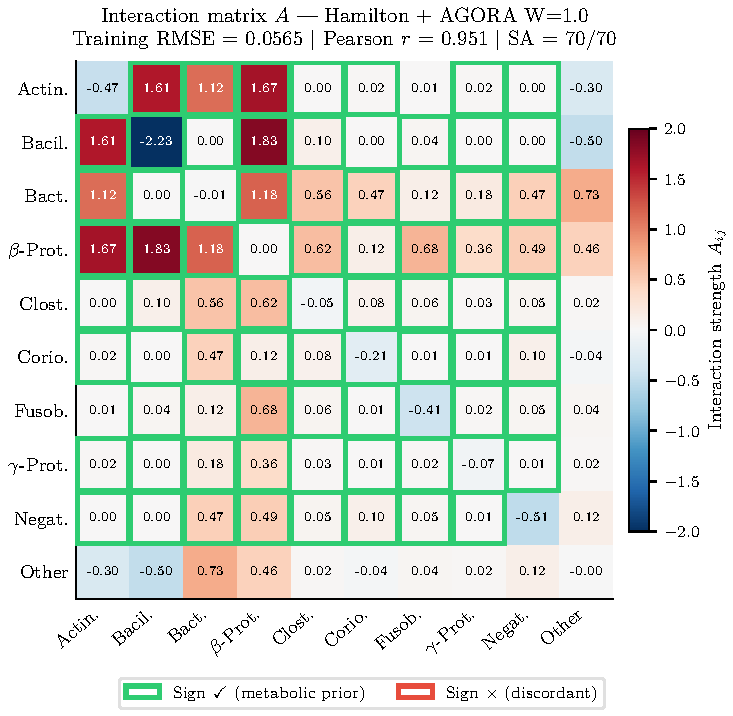
\includegraphics[width=0.72\textwidth]{dieckow_A_matrix.pdf}
  \caption[Fitted in-vivo interaction matrix]{Fitted interaction matrix $\bA$
  (Hamilton, full prior, all $10$ patients). Blue: competition; red: facilitation.
  Diagonals $A_{ii}<0$. Marks: sign agreement (\checkmark) / disagreement ($\times$)
  with the metabolic prior; full-model agreement $70/70$ ($100\%$). The dominant
  red block is the early-coloniser co-aggregation core.}
  \label{fig:dieckow_A}
\end{figure}

The asymmetric gLV ($\alpha{=}0.25$, best model; Table~\ref{tab:dieckow_loo})
recovers the same dominant structure as the Hamilton result, while the directed
representation reveals asymmetric facilitation absent from the symmetric prior
(Figure~\ref{fig:dieckow_glv_A}).

\begin{figure}[htbp]
  \centering
  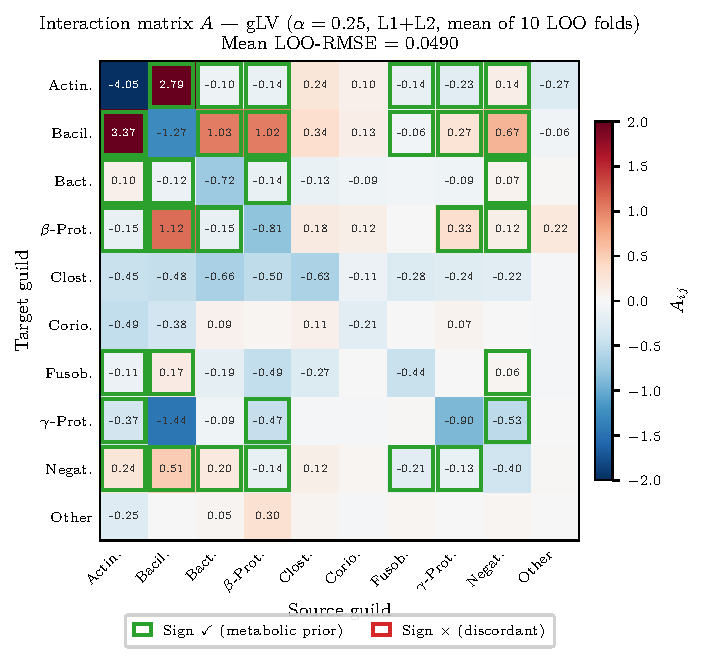
\includegraphics[width=0.68\textwidth]{dieckow_glv_Amatrix_thesis.pdf}
  \caption[Fitted in-vivo gLV interaction matrix]{Fitted interaction matrix
  $\bA$ (asymmetric gLV, $\alpha{=}0.25$, L1+L2 prior, mean of $10$ LOO folds,
  mean LOO-RMSE $= 0.0490$).
  Blue: competition; red: facilitation. Diagonals $A_{ii}<0$.
  Green borders: sign agreement with metabolic prior (L1+L2);
  red borders: discordant entries. Annotated values shown for $|A_{ij}|>0.05$.
  The early-coloniser co-aggregation block (Actin./Bacil./Bact./$\beta$-Prot.)
  dominates, consistent with the Hamilton result (Figure~\ref{fig:dieckow_A}).}
  \label{fig:dieckow_glv_A}
\end{figure}

The annotated entries reveal three features invisible to the symmetric Hamilton fit.
\emph{Bacillaceae as hub}: the Actin.--Bacil.\ mutual facilitation
($A_{\text{Bacil.,Actin.}}=+3.37$, $A_{\text{Actin.,Bacil.}}=+2.79$) is an order
of magnitude above any other pair; Bacillaceae additionally facilitates
$\beta$-Proteobacteria ($+1.02$), Bacteroidetes ($+1.03$), and Negativicutes
($+0.68$).
\emph{Sign-asymmetric $\gamma$-Proteobacteria}: although Bacillaceae mildly
facilitates $\gamma$-Proteobacteria ($+0.27$), $\gamma$-Proteobacteria strongly
suppresses Bacillaceae in return ($-1.44$, reversed sign) --- a directed antagonism
the symmetric model cannot represent.
\emph{Clostridiaceae broad suppressor}: all ten outgoing interactions are negative
(strongest $A_{\text{Clost.,Bact.}}=-0.66$), a profile that collapses into the
background competition term of the symmetric fit. The strongest diagonal entry is
Actinobacteria self-regulation ($A_{\text{Actin.,Actin.}}=-4.05$).

\begin{figure}[htbp]
  \centering
  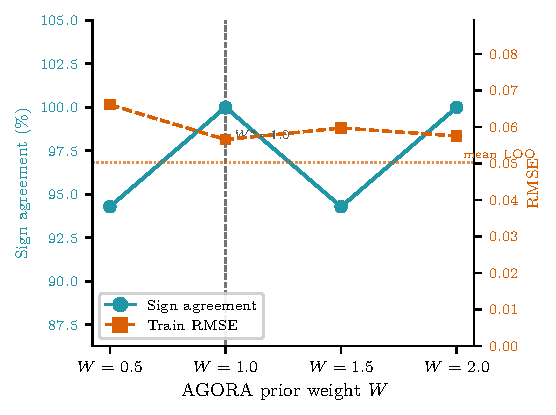
\includegraphics[width=0.6\textwidth]{fig_w_sweep_thesis.pdf}
  \caption[AGORA weight sweep: sign agreement and RMSE vs.\ $W$]{Effect of AGORA
  prior weight $W$ on sign agreement (teal, left axis) and training RMSE (orange,
  right axis). $W^*{=}1.0$ is the \emph{first} weight to achieve $100\%$ sign
  agreement ($70/70$ pairs) and simultaneously the one with the lowest training RMSE
  ($0.057$); $W{=}2.0$ also reaches $100\%$ but at higher RMSE ($0.058$). The mean
  LOO-RMSE at $W{=}1.0$ (dotted) confirms that full sign consistency is achieved
  without over-fitting.}
  \label{fig:w_sweep}
\end{figure}

\subsection{Out-of-sample generalisation}
\label{sec:dieckow_loo}

Across all variants (Table~\ref{tab:dieckow_loo}), every mechanistic model
decisively beats the ecological null: the best LOO-BC of $0.147$ is $47.7\%$ below
the persistence null ($0.281$). The sign prior improves the Hamilton model
monotonically (no prior $0.0595\to$ L1+L2 $0.0516\to$ MICOM $0.0502$, the best
Hamilton variant), and the overall best is the asymmetric gLV with $\alpha=0.25$
(L1+L2, RMSE $0.0490\pm0.016$) --- its extra directed freedom slightly outweighs
the symmetric sign constraint for this dataset. MICOM raises sign agreement to a
perfect $72/72$ at a $5$--$6\%$ RMSE cost relative to that best gLV, a
consistency-vs-accuracy trade-off discussed below. The fully Bayesian MDSINE2
collapses to $\bA\approx0$ under only three time points (LOO-RMSE $0.0552$, $13\%$
worse than gLV $\alpha{=}0.25$), confirming that \emph{sign-prior regularisation
outperforms Bayesian sparsity-induction when $T$ is small} --- the operative regime
for clinical microbiome series. The NSP variant ($0.091$) is $1.9\times$ worse,
its latent warm-up cost not repaid on this short horizon.

\begin{table}[htbp]
  \centering\small
  \begin{tabular}{@{}llccc@{}}
    \toprule
    Model & Layer & SA & LOO-RMSE & LOO-BC\\
    \midrule
    Hamilton (no prior)        & ---         & ---            & $0.0595$ & ---\\
    gLV free (asymmetric)      & ---         & ---            & $0.0588$ & $0.154$\\
    Hamilton L1+L2             & L1+L2       & $94\%$         & $0.0516$ & $0.155$\\
    Hamilton +AGORA v1         & L1+L2+L3    & $94\%$         & $0.0562$ & $\mathbf{0.147}$\\
    \textbf{gLV $\alpha{=}0.25$} & \textbf{L1+L2} & $97\%$    & $\mathbf{0.0490}$ & ---\\
    gLV +MICOM ($\alpha{=}0.25$) & L1+L2+L3-MC & $\mathbf{100\%}$ & $0.0516$ & ---\\
    Hamilton +MICOM            & L1+L2+L3-MC & $\mathbf{100\%}$ & $0.0502$ & ---\\
    \midrule
    NSP IFT v2                 & L1+L2       & ---            & $0.0906$ & ---\\
    MDSINE2 (Bayesian gLV)     & Bayesian    & ---            & $0.0552^\dagger$ & ---\\
    \bottomrule
    \multicolumn{5}{@{}l}{\small $^\dagger$8/10 folds; $\bA\approx0$ (insufficient
    Bayesian evidence at $T{=}3$). Null BC: persistence $0.281$.}
  \end{tabular}
  \caption[LOO cross-validation across model variants]{LOO cross-validation. SA:
  sign agreement on constrained pairs. Best values in bold. Sign-prior
  regularisation improves the Hamilton model monotonically; MICOM gives perfect
  sign agreement.}
  \label{tab:dieckow_loo}
\end{table}

\begin{figure}[htbp]
  \centering
  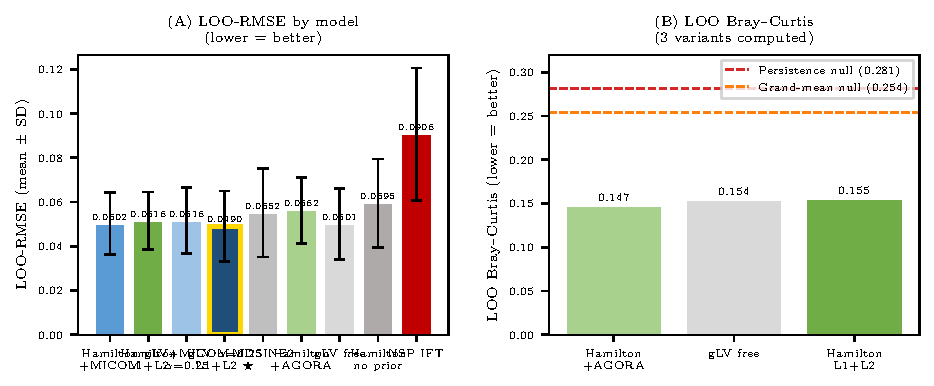
\includegraphics[width=0.80\textwidth]{dieckow_loo_bc.pdf}
  \caption[LOO Bray--Curtis across models]{LOO Bray--Curtis for all variants vs.\
  null models (dashed: persistence $0.281$, grand-mean $0.254$). Every ODE model
  substantially beats both nulls; the full-prior Hamilton attains the lowest BC
  ($0.147$).}
  \label{fig:dieckow_loo}
\end{figure}

\begin{figure}[p]
  \centering
  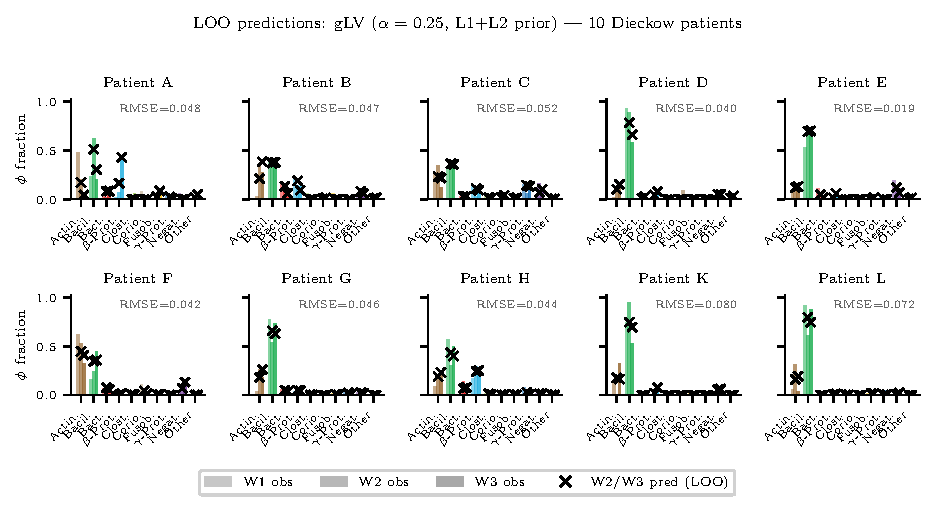
\includegraphics[width=0.70\textwidth,height=0.50\textheight,keepaspectratio]{dieckow_loo_fits_thesis.pdf}
  \caption[Per-patient LOO predictions: gLV ($\alpha{=}0.25$, L1+L2 prior)]{Per-patient
  leave-one-out predictions for all $10$ Dieckow patients.
  Bars: observed guild fractions at W1 (light), W2 (mid), W3 (dark).
  Crosses ($\times$): LOO-predicted W2 and W3 from the best-model gLV
  ($\alpha{=}0.25$, L1+L2 prior, mean RMSE $= 0.0490$); the held-out patient's
  $\bb^{(p)}$ is fit from W1 only and $\bA$ is frozen from the other 9 patients.
  The model tracks the dominant early-coloniser composition (Actinobacteria,
  Bacilli) across CT1 patients and the Bacteroidia/Fusobacteriia-enriched CT2
  composition, with largest errors at patients with atypical trajectories (K, L).}
  \label{fig:dieckow_loo_fits}
\end{figure}

\subsection{Is mechanistic structure necessary?}
\label{sec:dieckow_benchmark}

Table~\ref{tab:dieckow_loo} compares mechanistic variants among themselves,
but leaves open whether the ecological structure is needed at all. To test this
we benchmarked the gLV model against two baseline families under the identical
LOO one-step-ahead protocol: classical ML regression (Random Forest, Ridge,
LASSO, plus persistence and train-mean references) and modern generative models
(a conditional DDPM and conditional Flow Matching, the ODE-based successor to
diffusion). The mechanistic model wins decisively
(Figure~\ref{fig:dieckow_benchmark}): gLV attains LOO-RMSE $\approx0.05$,
$1.8\times$ below the best ML baseline (Random Forest $0.091$) and $2$--$3\times$
below the generative models (Flow Matching $0.107$, DDPM $0.166$). The gap holds
per patient --- gLV achieves the lowest RMSE on all $10$ held-out patients against
every competitor (one-sided Wilcoxon signed-rank $p=0.001$, the floor at $n=10$).

Two controls localise the cause to the data regime. Flow Matching beats DDPM by
$36\%$ --- the ODE formulation's training-stability advantage over the stochastic
reverse process --- yet both still lose to gLV; and augmenting the ML training set
with diffusion-sampled trajectories \emph{degrades} Ridge and Random Forest,
confirming that with only $18$ real transitions a generative model injects noise
rather than recovering the dynamics. With $T=3$ time points, encoding the
interaction structure is worth more than any amount of model flexibility --- the
same small-$T$ lesson as the MDSINE2 collapse (Table~\ref{tab:dieckow_loo}).

\begin{figure}[htbp]
  \centering
  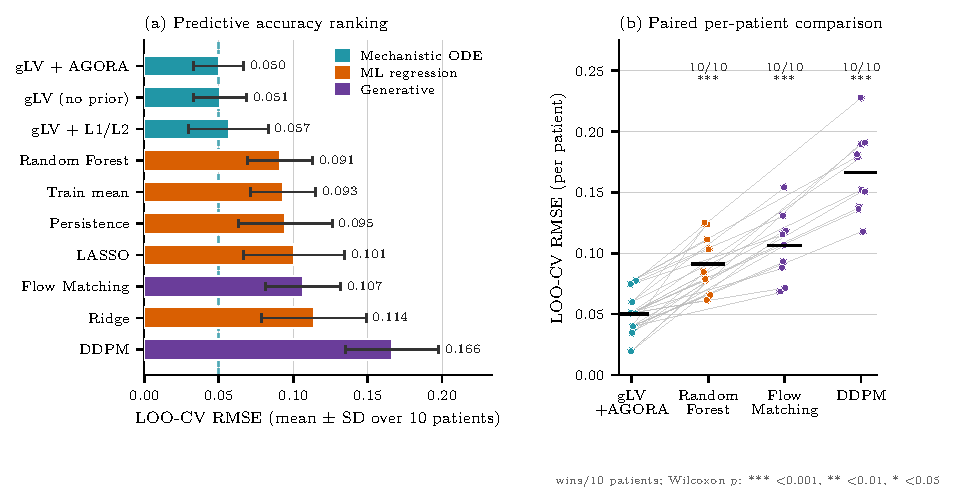
\includegraphics[width=0.72\textwidth]{dieckow_benchmark.pdf}
  \caption[gLV vs.\ ML and generative baselines]{\textbf{Mechanistic structure
  beats data-driven and generative baselines on LOO prediction.}
  \textbf{(a)}~LOO-CV RMSE (mean $\pm$ SD over the $10$ patients) for the
  one-step-ahead guild-composition task, grouped by family: mechanistic ODE (gLV
  variants), ML regression, and generative models (conditional Flow Matching and
  DDPM). \textbf{(b)}~Paired per-patient comparison of the best model against one
  representative of each competing family; each grey line links the two RMSE
  values for one held-out patient. gLV wins on all $10$ patients against every
  competitor (one-sided Wilcoxon signed-rank $p=0.001$, the minimum attainable at
  $n=10$).}
  \label{fig:dieckow_benchmark}
\end{figure}

\subsection{Sign, not magnitude --- the central finding}
\label{sec:dieckow_signmag}

Two results jointly establish the thesis's organising claim. First, a
\emph{quantitative} Gaussian prior that ties $A_{ij}$ to the FBA flux magnitude
($A_{ij}\sim\mathcal{N}(c\,\Phi_{ij},\sigma^2)$, MacArthur-style) \emph{fails
entirely}, recovering correct signs for only $4$--$11$ of $70$ pairs at any
concentration $c$: FBA flux magnitude is not ecologically predictive. Second, the
\emph{sign}-only prior is both accurate (Table~\ref{tab:dieckow_loo}) and stable:
across the $10$ LOO folds, $31/45$ off-diagonal pairs have perfect sign consistency
(SC$=1.00$), $40/45$ reach SC$\geq0.90$, and only one falls below $0.70$
(Figure~\ref{fig:dieckow_stability}). Prior-pinned pairs keep SC$\geq0.80$ even
when their magnitude is negligible --- the prior fixes direction where the data are
silent. This is why the penalty in Eq.~\eqref{eq:dieckow_penalty} constrains sign
and never magnitude: it injects exactly the part of the metabolic evidence that
transfers (the direction of the interaction) and none of the part that does not
(its flux-unit size).

\begin{figure}[htbp]
  \centering
  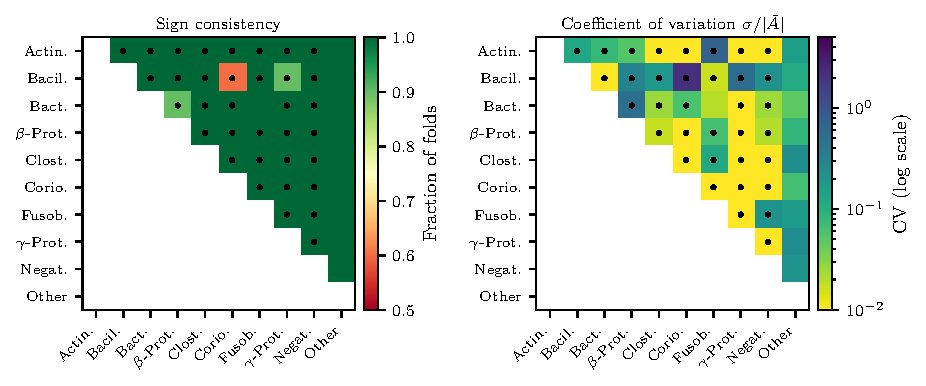
\includegraphics[width=0.72\textwidth]{fig_loo_stability.pdf}
  \caption[LOO-CV interaction-sign consistency]{Leave-one-out sign consistency
  of the fitted $\bA$.
  \textbf{(a)}~Fraction of $10$ LOO folds in which each pair $(i,j)$ recovers
  the same sign as the full-data MAP; $31/45$ pairs reach SC$=1.00$, $40/45$
  reach SC$\geq0.90$.
  \textbf{(b)}~Coefficient of variation ($\sigma/|\mu|$) of $A_{ij}$ across
  folds; prior-pinned pairs (dots) remain stable even when magnitudes are small.}
  \label{fig:dieckow_stability}
\end{figure}

A direct test of independence confirms that the cross-feeding directions are
genuine data signal rather than an artefact of the prior.  When the sign
penalty is removed entirely and the symmetric Hamilton model is re-fitted
without guidance, it still recovers $78.6\%$ (11/14 pairs) of the
AGORA-predicted cross-feeding signs --- significantly above a cell-label
permutation null ($\bar p_{\rm null}=37.7\%$,
$p=4\times10^{-4}$, $z=+3.79$, $n_{\rm perm}=10{,}000$).
The asymmetric gLV model shows no such effect ($p=0.96$, $z=-1.47$):
the Hamilton symmetry constraint mediates the metabolic--ecological
correspondence.  Only cooperative (cross-feeding) directions are validated;
competitive interactions carry no detectable signal across patients,
consistent with competition being shaped by local context rather than
conserved metabolic architecture.

\subsection{Patient structure and community type}
\label{sec:dieckow_struct}

The shared $\bA$ captures patient-independent guild ecology; patient-level
variation is absorbed by the growth vectors $\bb^{(p)}$. A PCA of the fitted
$\hat\bb^{(p)}$ (Figure~\ref{fig:dieckow_bpca}) separates CT1 from CT2 along PC1
\emph{without} community-type supervision (CT1: higher Actinobacteria/Bacilli
intrinsic rates; CT2: higher Fusobacteriia), and the LOO predictions preserve the
CT1/CT2 discriminant (LDA accuracy $90\%$, only the atypical Patient~A
misclassified) while spanning the observed compositional manifold rather than
collapsing to the mean. Off-diagonal interactions are on average twice as strong as
intrinsic rates ($\overline{|A_{\mathrm{off}}|}=0.35$ vs.\ $\overline{|b|}=0.18$):
community ecology dominates individual guild growth here.


\subsection{Network centrality and keystone structure}
\label{sec:dieckow_network}

Reading the fitted $\bA$ as a directed weighted graph~\cite{Freilich2020Inference, May1972Stability}
exposes which guilds organise the community (Figure~\ref{fig:dieckow_centrality}). \emph{Actinobacteria} is the
dominant hub on every measure: highest outgoing influence ($5.6$), the largest
positive net effect (out minus in, $+2.0$), and top centrality rank --- a net
\emph{source} that drives the early-coloniser core. \emph{Bacilli} is the most
\emph{vulnerable} guild (incoming strength $8.2$): abundant but strongly
acted-upon. The most ecologically interesting guild is \emph{Fusobacteriia}, which
carries a large \emph{keystone gap} (centrality rank well above its abundance rank,
gap $+2$): it is influential out of proportion to how much of it there is --- the
quantitative signature of a low-abundance bridging organism, the in-vivo guild-level
echo of the \textit{F.~nucleatum} bridging role seen in vitro
(Section~\ref{sec:heine_rewiring}). These rankings are stable across the LOO folds,
so the keystone ordering is a property of the inferred ecology, not of any single
patient.

\begin{figure}[htbp]
  \centering
  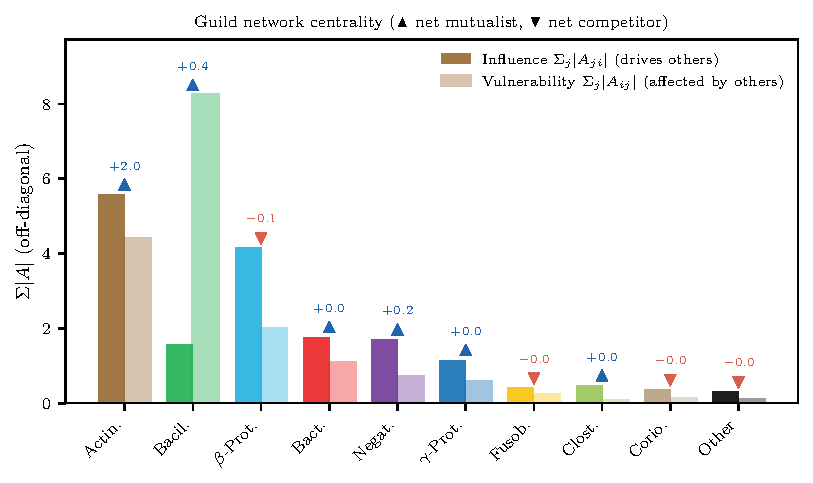
\includegraphics[width=0.70\textwidth]{dieckow_centrality.pdf}
  \caption[Guild network centrality]{Guild interaction-network centrality from the
  fitted $\bA$. Actinobacteria is the top influencer / net source; Bacilli is the
  most vulnerable (highest incoming strength); Fusobacteriia carries the largest
  keystone gap (central despite low abundance --- a bridging guild).}
  \label{fig:dieckow_centrality}
\end{figure}

\begin{figure}[htbp]
  \centering
  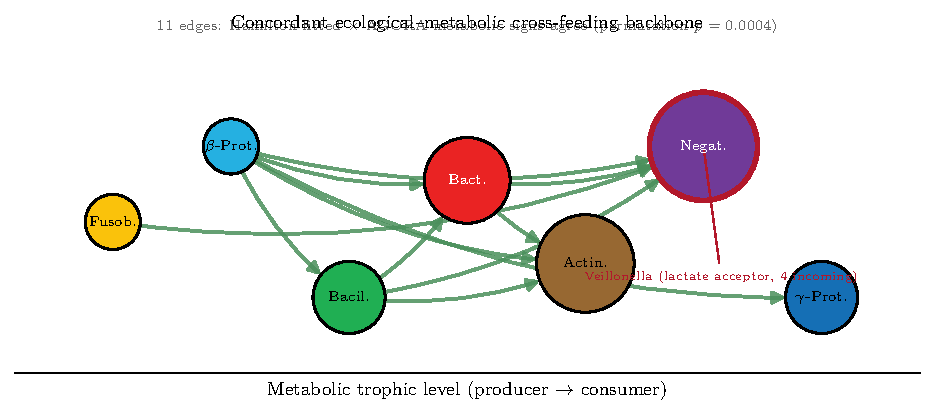
\includegraphics[width=0.70\textwidth]{fig_network_backbone_thesis.pdf}
  \caption[Cross-cohort concordant interaction backbone]{Concordant interaction
  backbone across Dieckow ($N=10$) and Botelho ($N=15$) cohorts.
  Strong pairs ($|\hat A_{ij}|>0.1$ in both fits) are shown; $8/9$ agree in sign
  ($p\approx0.02$, permutation). The Actinobacteria hub is the most concordant
  node (5/5 edges consistent), confirming its role as a structural hub independent
  of cohort.}
  \label{fig:dieckow_backbone}
\end{figure}

\begin{figure}[htbp]
  \centering
  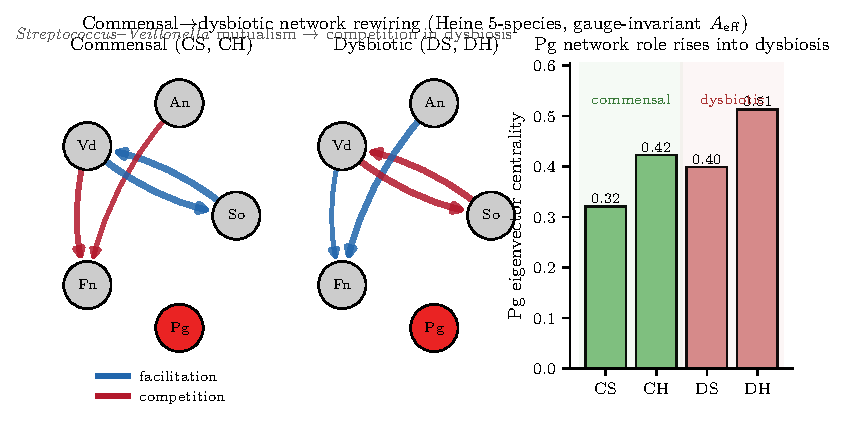
\includegraphics[width=0.70\textwidth]{fig_network_rewiring_thesis.pdf}
  \caption[CS$\to$DH interaction network rewiring]{Network rewiring from
  Commensal Static (CS) to Dysbiotic HOBIC (DH) in the Heine 5-species system.
  Edges that gain strength ($|\Delta A_{ij}|>0.2$) are highlighted; the
  \textit{Pg}--\textit{Fn} positive edge and the competitive suppression of
  \textit{An}/\textit{So} are the dominant rewired pairs.}
  \label{fig:dieckow_rewiring}
\end{figure}

%==============================================================================
\section{External Validation: Peri-Implant Dysbiosis}
\label{sec:dieckow_joshi}
%==============================================================================

To test transfer beyond the calibration cohort, the Dieckow-derived dysbiosis
ordering is applied to $127$ independent cross-sectional peri-implant samples
(Joshi et al.~\cite{joshi2025}: Health/Mucositis/Peri-implantitis). A guild-level
red/green dysbiosis ratio,
$\log(\phi_{\mathrm{Fuso}}+\phi_{\mathrm{Bact}}+\phi_{\mathrm{Clos}})-
\log(\phi_{\mathrm{Bac}}+\phi_{\mathrm{Act}}+\phi_{\mathrm{Neg}})$,
cleanly separates the diagnostic groups (Table~\ref{tab:dieckow_joshi};
Figure~\ref{fig:dieckow_joshi}): Health and Mucositis sit together (mean $-2.09$
vs.\ $-1.74$) while Peri-implantitis shifts sharply positive ($+0.53$).
Kruskal--Wallis $H=34.7$, $p<10^{-4}$; severity correlation Spearman $\rho=0.46$
($p=5\times10^{-8}$, $N=127$), rising to $\rho=0.59$ for the binary
Health-vs-PI contrast. The model thus orders dysbiosis correctly on data it never
saw; the moderate three-way $\rho$ reflects the near-identity of Health and
Mucositis in this five-genus space, which would need additional pathogens to
resolve.

\begin{table}[htbp]
  \centering\small
  \begin{tabular}{@{}lcccc@{}}
    \toprule
    Diagnosis & $n$ & Mean R/G & Median R/G & vs.\ Health\\
    \midrule
    Health           & $56$ & $-2.09$ & $-1.88$ & ---\\
    Mucositis        & $39$ & $-1.74$ & $-1.65$ & $p=0.47$\\
    Peri-implantitis & $32$ & $+0.53$ & $+0.76$ & $p<10^{-4}$\\
    \bottomrule
    \multicolumn{5}{@{}l}{\small Kruskal--Wallis $H=34.7$, $p<10^{-4}$; Spearman
    $\rho=0.46$, $p=5\times10^{-8}$.}
  \end{tabular}
  \caption[Peri-implant dysbiosis ordering]{Guild-level R/G dysbiosis ratio by
  diagnosis (Joshi et al., $127$ samples). The Dieckow-derived ordering separates
  peri-implantitis from health/mucositis on independent cross-sectional data.}
  \label{tab:dieckow_joshi}
\end{table}

\begin{figure}[htbp]
  \centering
  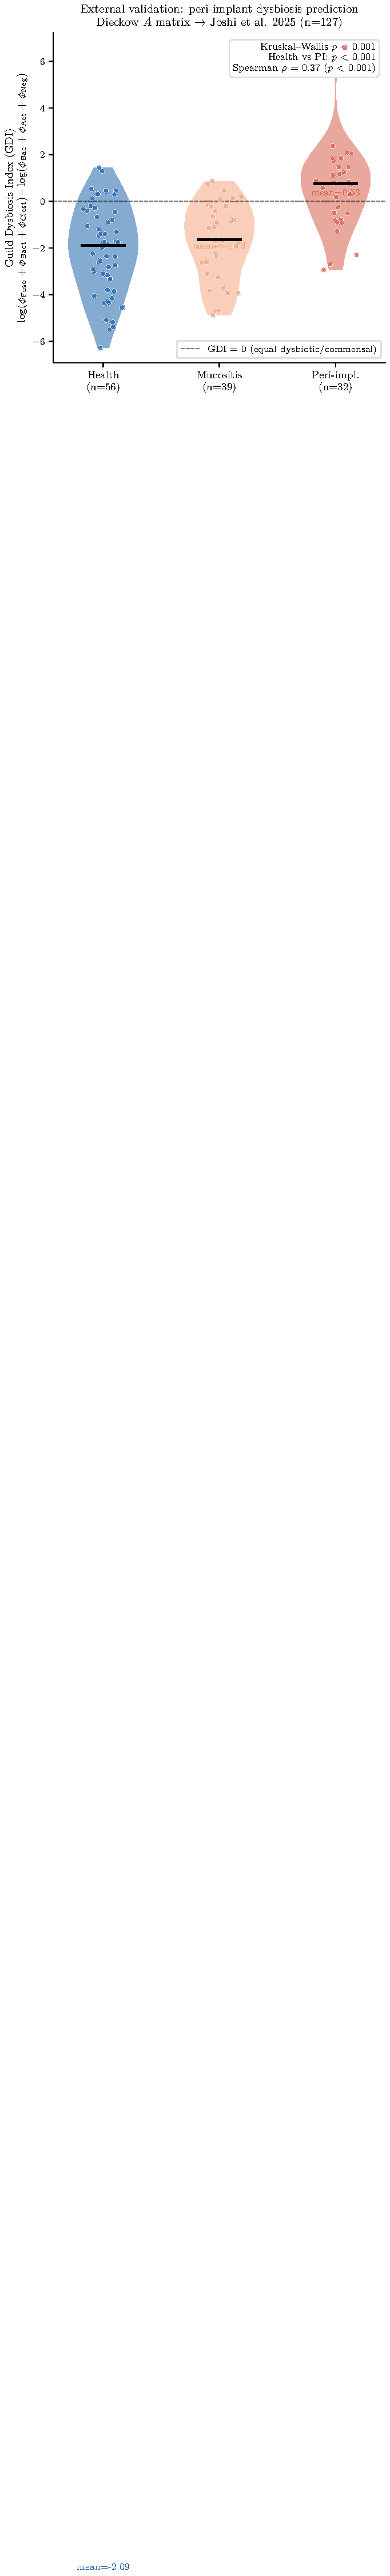
\includegraphics[width=0.68\textwidth,height=0.36\textheight,keepaspectratio]{dieckow_joshi.pdf}
  \caption[Peri-implant dysbiosis attractor analysis]{R/G dysbiosis ratio across
  Health, Mucositis and Peri-implantitis (Joshi et al., $N=127$). Peri-implantitis
  separates with a large positive shift; severity correlation $\rho=0.46$
  ($p=5\times10^{-8}$).}
  \label{fig:dieckow_joshi}
\end{figure}

\begin{figure}[htbp]
  \centering
  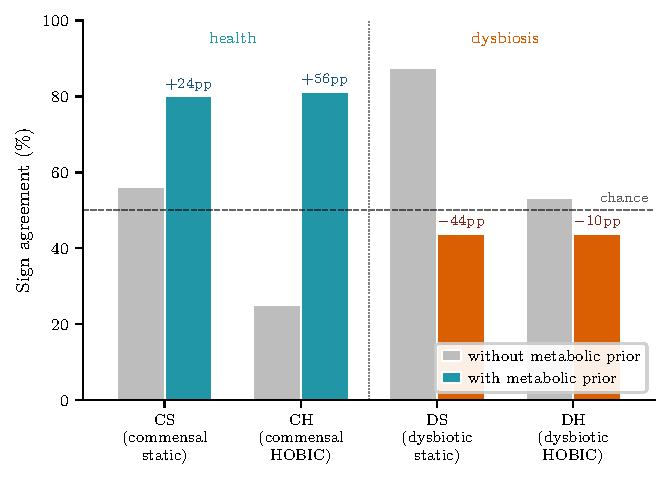
\includegraphics[width=0.72\textwidth]{fig_prior_asymmetry.pdf}
  \caption[Prior sign agreement by community state]{Sign agreement between the
  AGORA-predicted cross-feeding signs and the TMCMC posterior, with and without
  the metabolic prior, across the four Heine attractors.  Health states (CS, CH)
  gain $+24$ and $+56$ percentage points from the prior; dysbiotic states (DS, DH)
  lose $-44$ and $-10$ pp, falling below chance.  The metabolic prior is
  \emph{informative for health-associated ecology and actively harmful for
  dysbiotic ecology}, where pathogenic interactions override the commensal
  cross-feeding template.}
  \label{fig:prior_asymmetry}
\end{figure}

%==============================================================================
\section{Discussion}
\label{sec:dieckow_discussion}
%==============================================================================

The in-vivo analysis confirms and sharpens the thesis's organising idea. Metabolic
flux-balance evidence is predictive \emph{as a sign constraint but not as a
magnitude} (the quantitative MacArthur prior fails outright), and a sign-only prior
is what generalises: it improves out-of-sample prediction monotonically, stabilises
the inferred network across folds, and lets community FBA (MICOM) reach perfect
sign agreement. That MICOM's full consistency comes at a small RMSE cost relative
to the best gLV reflects the honest tension between biological self-consistency and
raw predictive accuracy at this cohort size, not a failure of either. The framework
also out-predicts a fully Bayesian gLV (MDSINE2), which collapses to no interactions
under three time points --- the practically important lesson that mechanistic sign
priors substitute for the data a Bayesian model would otherwise need.

The principal limitations are statistical and structural. With $N=10$ patients the
AGORA/MICOM improvement over L1+L2 is real but only marginally significant
($p\approx0.07$--$0.08$), so the perfect-sign-agreement result should be read as a
consistency check rather than a powered effect. The Hamilton symmetry constraint
$A_{ij}=A_{ji}$ excludes genuinely asymmetric ecological interactions --- precisely
where the asymmetric gLV gains its edge --- and the prior is curated for a
caries-recovery context whose transfer to other disease states is untested beyond
the peri-implant ordering shown above. These motivate the spatial extension of
Chapter~\ref{ch:integration}, where the same prior-regularised interactions are
carried into a depth-resolved reaction--diffusion model and confronted with FISH
imaging.
A further limitation is that the magnitude of AGORA2-derived cross-feeding
fluxes cannot be directly calibrated to the gLV interaction scale without
additional kinetic parameters (Monod half-saturation constants); recovering
absolute interaction strengths from GEM stoichiometry remains an open problem
in the field~\cite{Rath2024GEMReliability,Mustri2025GLVABreakdown}.

\paragraph{Statistical power and the sign enrichment as primary evidence.}
The marginal significance of the MICOM--gLV RMSE comparison ($p\approx0.07$,
$N=10$) is expected: for a medium effect size ($d=0.5$) and $N=10$ a
two-sample test has power $\approx0.30$, so the study is structurally
underpowered for this particular comparison. The primary quantitative
evidence is therefore the permutation-based cross-feeding sign enrichment
reported above, which aggregates over all $45\times10$ fold-pair combinations
and is independent of cohort size in this different sense. A complementary
robustness check --- neutral-initialised no-prior LOO starting from
$\mathbf{A}=\mathbf{0}$, which eliminates any warm-start bias --- yields
$\mathrm{SA}=71.4\%$ ($p=0.027$, permutation test, $n_\pi=10^4$), confirming
that the cross-feeding enrichment is data-driven and not an artefact of
warm-starting from the prior-fitted $\mathbf{A}$.

% \chapter{Integration and Outlook}
\label{ch:integration}

\section{Complementarity of the Two Frameworks}
\label{sec:integration_compare}

Chapters~\ref{ch:heine} and~\ref{ch:dieckow} attack the same problem --- inferring
species interactions from compositional time series under the Extended Hamilton
Principle --- from opposite ends of the controlled/clinical spectrum. They are
deliberately complementary rather than redundant (Table~\ref{tab:complementarity}).

\begin{table}[htbp]
  \centering\small
  \begin{tabular}{@{}lll@{}}
    \toprule
    \textbf{Aspect} & \textbf{Ch.~\ref{ch:heine} (Heine, in-vitro)} & \textbf{Ch.~\ref{ch:dieckow} (Dieckow, in-vivo)}\\
    \midrule
    Data           & in-vitro, controlled & in-vivo, clinical\\
    Dimension      & $5$ species          & $10$ class-level guilds\\
    Model          & Hamilton $\bphi$--$\bpsi$ (viability) & Hamilton replicator ($\bphi$ only)\\
    Inference      & Bayesian TMCMC (full posterior) & L-BFGS-B point estimate $+$ LOO\\
    Regulariser    & iteratively narrowed priors & metabolic FBA \emph{sign} prior\\
    Acceleration   & GPU \texttt{vmap} ($\sim$$200\times$) & JAX-JIT autodiff\\
    Validation     & $4$ conditions $+$ held-out pH & $10$-fold LOO $+$ Joshi external\\
    \bottomrule
  \end{tabular}
  \caption[Complementarity of the in-vitro and in-vivo frameworks]{The two
  inference frameworks are complementary: controlled identifiability and full
  posteriors in vitro; clinical relevance and metabolic-prior identifiability in
  vivo.}
  \label{tab:complementarity}
\end{table}

The in-vitro setting (Chapter~\ref{ch:heine}) trades realism for control. With
defined strains, replicated conditions, and measured viability, it can afford a
\emph{full Bayesian posterior} over a $15$-parameter symmetric matrix and a
$\bphi$--$\bpsi$ model that resolves living from total biomass --- at the cost of
applying only to a five-species laboratory consortium. The data are rich enough
that the regulariser need only be an iteratively narrowed prior; the posterior
itself recovers biological sparsity without metabolic input.

The in-vivo setting (Chapter~\ref{ch:dieckow}) inverts every term of that trade.
Ten guilds, three time points, and ten patients leave the interaction matrix
underdetermined, so a point estimate replaces the posterior and an external
\emph{metabolic sign prior} supplies the identifiability the data cannot. What the
clinical setting loses in statistical luxury it gains in reach: out-of-sample LOO
generalisation and transfer to an independent peri-implant cohort.

Crucially, the two share a backbone. Both are replicator dynamics on the simplex
with a symmetric interaction matrix derived from the same variational principle
(Chapter~\ref{ch:theory}), and both find that interaction \emph{sign} is the
robust, transferable quantity --- recovered emergently from rich in-vitro data and
imposed as a prior on sparse in-vivo data. Read together they form a single
pipeline: controlled in-vitro estimation calibrates the model and validates the
sign structure that the in-vivo prior then exploits where data are scarce, and the
spatial extension of this chapter carries the same interactions into depth-resolved
prediction.
A structural echo of this complementarity is visible in the COMSTAT biofilm metrics:
the roughness coefficient $R_a$ of \textit{P.~gingivalis} is significantly higher
in the dysbiotic-HOBIC condition than in the commensal one (Mann--Whitney
$p < 0.001$), which mirrors the Hamilton posterior showing a stronger
Fn$\to$Pg interaction in DH ($\mathrm{P}(a_{Fn\to Pg}>0)=1.00$) versus CH
($\mathrm{P}=0.82$) --- a suggestive co-variation between spatial surface roughness
and inferred network interaction strength, consistent with the picture that
stronger Fn facilitation allows Pg to form more structurally complex colonies.

A deeper complementarity concerns what each framework \emph{measures}.
The Hamilton ODE equilibrium (300 posterior samples, uniform initialisation)
converges to Pg~$+$~Fn dominance
($\phi_\mathrm{Pg}^\mathrm{CH}\!\approx 0.49$; $\phi_\mathrm{Fn+Pg}^\mathrm{DH}\!\approx 1.0$),
yet COMSTAT shows near-uniform substrate coverage across all five species
($0.19$--$0.26$; $r = 0.07$ CH, $r = 0.52$ DH with the ODE).
The discrepancy is resolved by vertical stratification: competitive exclusion in the
mean-field model corresponds to depth-niche partitioning in the real biofilm,
which COMSTAT's 2-D projection cannot detect but FISH can (Section~\ref{sec:pde_fish}).
Figure~\ref{fig:hamilton_vs_comstat} shows the ODE--COMSTAT correlation explicitly.

\begin{figure}[htbp]
  \centering
  \includegraphics[width=0.74\textwidth]{fig_hamilton_vs_comstat.pdf}
  \caption[Hamilton ODE equilibrium vs COMSTAT substrate coverage]{Hamilton ODE
  equilibrium composition (posterior median, $n=300$ samples) versus COMSTAT
  substrate coverage fraction for all five species in CH and DH.
  The low correlation ($r=0.07$ CH, $r=0.52$ DH) reflects the fundamental
  difference between volume-averaged abundance (ODE) and 2-D areal coverage
  (COMSTAT), not a model failure.}
  \label{fig:hamilton_vs_comstat}
\end{figure}

\section{Towards a Unified Bayesian-Metabolic Framework}
\label{sec:integration_unified}

The two inference frameworks are, at present, methodologically disjoint: the
in-vitro analysis (Chapter~\ref{ch:heine}) produces a full Bayesian posterior but
uses only an uninformative, iteratively narrowed prior, while the in-vivo analysis
(Chapter~\ref{ch:dieckow}) injects the metabolic sign prior but collapses to a point
estimate. Their natural synthesis is a single scheme that does both --- a
\emph{metabolically-regularised TMCMC posterior}.

\paragraph{A unified objective.}
Concretely, the metabolic sign penalty $\calP(\bA;\bF)$ of
Eq.~\eqref{eq:dieckow_penalty} is a log-prior: $\log p_{\mathrm{sign}}(\bA) =
-\calP(\bA;\bF)$, the half-normal density that is flat for correct-sign entries and
quadratically suppresses sign violations in proportion to the metabolic evidence
$|F_{ij}|$. Adding it to the TMCMC prior of Section~\ref{sec:theory_tmcmc} gives the
tempered target
\begin{equation}
  p_m(\btheta) \;\propto\; p(\yobs\mid\btheta)^{\beta_m}\;
    \underbrace{p_0(\btheta)\,
    \exp\!\bigl[-\calP(\bA;\bF)\bigr]}_{\text{metabolically-informed prior}},
  \label{eq:unified}
\end{equation}
so the sampler explores the \emph{full} posterior --- credible intervals,
multimodality, model evidence --- while the metabolic prior supplies exactly the
identifiability that sparse clinical data lack. This directly targets the principal
limitation of Chapter~\ref{ch:dieckow} (the AGORA improvement was only marginally
significant at $N=10$, $p\!\approx\!0.07$): with posterior uncertainty made explicit,
the question shifts from a single point estimate to whether the metabolic prior
sharpens the posterior on the constrained entries, a quantity that remains
informative even in small cohorts. We ran exactly this coupling on the in-vitro
data --- a sign-prior-regularised TMCMC ($\sigma_{\mathrm{KEGG}}=0.15$ commensal,
$0.08$ dysbiotic) whose MAP matrix is scored against a KEGG/eHOMD net-flow matrix.
The result is informative precisely because it is \emph{asymmetric}: the metabolic
prior raises the MAP sign agreement in the commensal conditions (CS $56\!\to\!80\%$,
CH $25\!\to\!81\%$) but lowers it in the dysbiotic ones (DS $88\!\to\!44\%$,
DH $53\!\to\!44\%$). The prior aligns with health, where metabolite-mediated
mutualism organises the community, yet conflicts with dysbiosis, where the data
demand sign reversals --- concentrated on the \textit{F.~nucleatum} edges, where
shear-driven competition overrides metabolic mutualism --- that the caries-context
metabolic network does not encode. This recovers, in vitro, the very pattern the
in-vivo analysis made central: interaction sign is metabolically predictable in
health, but in dysbiosis the data must be allowed to override the prior.

\paragraph{Scaling and personalisation.}
With larger clinical series the Bayesian machinery quantifies heterogeneity a point
estimate hides; a hierarchical extension --- shared $\bA^{\mathrm{pop}}$ with
patient-specific deviations --- would partition community ecology from individual
variation. Personalising the prior via patient-specific MICOM fluxes $\bF^{(p)}$
would turn sign regularisation into a route toward individualised dysbiosis prediction.

\section{Spatial Extension: Reaction--Diffusion PDE}
\label{sec:integration_pde}

The $0$D model of Chapter~\ref{ch:heine} describes a well-mixed material point.
To resolve the depth stratification seen in confocal (FISH) imaging, we promote the
species fractions to fields $\phi_i(z,t)$ over the biofilm thickness $z\in[0,L]$ and
add molecular transport to the Hamilton reaction, giving a reaction--diffusion--advection
system in the long tradition of reaction--diffusion models of pattern formation and
biofilms~\cite{Turing1952Morphogenesis, Murray2003MathBiologyII, Kreft2001IbmBiofilm, Ward2003MathBiofilm}.

\subsection{Strong form}
\label{sec:pde_strong}
Each species field obeys
\begin{equation}
  \frac{\partial \phi_i}{\partial t}
  = \underbrace{D_i\,\frac{\partial^2 \phi_i}{\partial z^2}}_{\text{diffusion}}
    \;-\; \underbrace{u\,\frac{\partial \phi_i}{\partial z}}_{\text{advection}}
    \;+\; \underbrace{R_i(\bphi,\bpsi)}_{\text{NSP reaction}},
  \qquad i = 1,\dots,n,
  \label{eq:pde_strong}
\end{equation}
where $R_i$ is the per-point NSP reaction of Section~\ref{sec:theory_replicator}
(carrying the viability $\psi_i$, void fraction $\phi_0$, and constraint multiplier
$\gamma$), $D_i$ are species diffusivities, and $u$ is a common advective drift towards
the bulk. Diffusion and advection act on $\phi_i$ only; the reaction acts on the full NSP
state $\mathbf{g}(z)=(\phi_1,\dots,\phi_n,\phi_0,\psi_1,\dots,\psi_n,\gamma)$ at each $z$.

\paragraph{Boundary and initial conditions.}
At the substratum a no-flux (homogeneous Neumann) condition $\partial_z\phi_i|_{z=0}=0$
expresses the impermeable surface; at the biofilm--bulk interface a Dirichlet condition
$\phi_i(L,t)=\phi_{\mathrm{bulk},i}$ fixes the planktonic composition (taken as the
Day-1 median). The diffusivities $D_i$ and drift $u$ are structural parameters of
the model; with only $T=5$ FISH timepoints available (Days 1, 6, 10, 15, 21),
the temporal derivative $\partial_t\phi_i$ is too coarsely sampled to identify $D_i$
quantitatively by finite differencing~\cite{Stewart1998Diffusion}.
A PINN inverse fit to the same profiles (Section~\ref{sec:pde_fish}) yields
$D_i \approx 8\times10^{-4}$ (DH) and $D_i \approx 8\times10^{-3}$ (CH) in
normalised units, with advection $u$ reversing sign between conditions.

\subsection{Numerical scheme}
\label{sec:pde_numerics}
Equation~\eqref{eq:pde_strong} is discretised by the \emph{method of lines} with
\emph{Lie operator splitting} of the stiff reaction from the transport:
\begin{equation}
  \bphi^{\,n+1} \;=\; \mathcal{T}_{\Delta t}\bigl(\mathcal{R}_{\Delta t}(\bphi^{\,n})\bigr),
  \label{eq:splitting}
\end{equation}
a first-order ($\mathcal{O}(\Delta t)$) splitting.

\paragraph{Reaction substep $\mathcal{R}$.}
At every grid node the NSP material-point system is advanced by \emph{implicit Euler}
and solved with Newton's method ($n_{\mathrm R}=5$ iterations, internal step
$\Delta t_h=10^{-3}$), vectorised across nodes (one \texttt{vmap} over the $z$-axis).
Implicit integration is chosen because the reaction is stiff near the simplex boundary,
where the logarithmic barrier ($K_p=10^{-4}$) stiffens the Jacobian.

\paragraph{Transport substep $\mathcal{T}$ (diagonal baseline).}
Diffusion uses a second-order central stencil; advection uses first-order upwind, giving a
globally first-order ($\mathcal{O}(\Delta z)$) spatial scheme. The no-flux wall is imposed
by a ghost node; the Dirichlet bulk value is written into the last node. Explicit Euler
advances the transport; the numerical diffusion $\tfrac12 u\,\Delta z$ must be kept below
the physical $D_i$, which constrains $\Delta z$.

\subsection{Simplex preservation: volume-filling cross-diffusion}
\label{sec:pde_xdiff}
The diagonal scheme diffuses each $\phi_i$ independently and then closes the simplex by
re-setting $\phi_0=1-\sum_i\phi_i$ and clipping to $[0,1]$; this is a deliberate but
\emph{non-conservative} approximation. A simplex-preserving formulation replaces it with a
\emph{volume-filling} (size-exclusion) cross-diffusion flux~\cite{PainterHillen2002VolumeFilling}
\begin{equation}
  J_i = -D_i\Bigl[(1-\rho)\,\partial_z\phi_i + \phi_i\,\partial_z\rho\Bigr],
  \quad \rho=\sum_{j}\phi_j,
  \qquad
  \frac{\partial\phi_i}{\partial t} = -\partial_z J_i - u\,\partial_z\phi_i + R_i,
  \label{eq:xdiff}
\end{equation}
discretised conservatively by finite volumes (fluxes evaluated on cell faces). The flux is
\emph{degenerate}, $J_i\to0$ as $\rho\to1$ or $\phi_i\to0$, so $0\le\phi_i,\rho\le1$ are
preserved \emph{by construction} and $\phi_0=1-\rho$ is a genuine void fraction rather than
a patched residual. Crucially, cross-coupling enters only through the shared crowding
gradient $\partial_z\rho$, so the model retains exactly $n$ free self-mobilities $D_i$
(no $n^2$ blow-up) and remains identifiable from $z$-profiles. Both schemes share the same
sign structure and fixed points; the cross-diffusion form is used wherever conservation and
boundedness matter.

\subsection{Stability, conservation, and verification}
\label{sec:pde_verification}
The explicit transport substep is conditionally stable. The diffusive and advective
Courant--Friedrichs--Lewy (CFL) limits
\begin{equation}
  \Delta t \;\le\; \tfrac12\,\frac{\Delta z^2}{\max_i D_i}
  \qquad\text{and}\qquad
  \frac{u\,\Delta t}{\Delta z} \;\le\; 1
  \label{eq:cfl}
\end{equation}
must both hold; the cross-diffusion solver enforces the diffusive bound automatically
(clamping $\Delta t$ to $0.9$ of the limit), and production runs are reported at a fixed
sub-CFL $\Delta t$ satisfying both.

Verification in a closed-box setting (reaction off, $u=0$) confirms $\mathcal{O}(\Delta z^2)$ interior convergence, $\mathcal{O}(\Delta z)$ boundary order at the ghost-node wall, and exact mass conservation for the finite-volume cross-diffusion scheme; the diagonal scheme drifts by $+2.2\times10^{-3}$ in the sub-critical regime and overshoots $\rho>1$ when crowded. Full convergence plots and conservation table are in Appendix~\ref{app:pde}.

\paragraph{Qualitative model--data comparison.}
Figure~\ref{fig:pde_ch_profile} shows the CH attractor depth profile from the
cross-diffusion PDE alongside the corresponding FISH $z$-profile (Day~1 median,
normalised), using diffusivities fit to the commensal-HOBIC data
($D_{\mathrm{CH}}$, loss $\approx 0.015$, volume-filling cross-diffusion scheme,
$N_z=32$).  The model reproduces the qualitative features: \textit{S.~oralis}
dominates the outer layer and \textit{P.~gingivalis} is confined near the
substrate, consistent with the depth-ordering and Manders results of
Section~\ref{sec:pde_fish}.  Quantitative agreement is limited by the coarse
temporal sampling ($T=5$ FISH timepoints), which prevents full identification of
the $D_i$ (Section~\ref{sec:pde_strong}); fitted values should be read as
order-of-magnitude estimates rather than measured transport coefficients.

\begin{figure}[htbp]
  \centering
  \includegraphics[width=0.74\textwidth]{fig_pde_ch_profile.pdf}
  \caption[PDE depth profile vs.\ FISH observation (CH attractor)]{%
  Qualitative comparison of the reaction--diffusion model and the FISH
  $z$-profile for the commensal-HOBIC (CH) attractor.
  \textbf{(a)}~FISH median depth profile (Day~1, $N_z=32$ bins, normalised
  relative abundance). \textbf{(b)}~Steady-state $z$-profile from the
  volume-filling cross-diffusion PDE with diffusivities fit to the CH
  $z$-profiles (loss $= 0.015$).
  The outer-layer dominance of \textit{S.~oralis} (blue) and inner
  sequestration of \textit{P.~gingivalis} (red) are reproduced qualitatively;
  quantitative fits await continuous live-imaging data for full $D_i$
  identification.}
  \label{fig:pde_ch_profile}
\end{figure}

\subsection{Empirical depth structure from 3-D FISH imaging}
\label{sec:pde_fish}
The spatial model is ultimately answerable to the real depth structure of the
biofilm. We extracted the full three-dimensional $(x,y,z)$ organisation of the five
species from the Heine HOBIC FISH dataset --- $84$ titanium fields of view across
all $11$ confocal \texttt{.lif} acquisitions, decoded \emph{per voxel} (without the
usual $xy$-averaging) into the five-species channels. Two findings, both resting on
billions of voxels, emerge and are the principal empirical result of the spatial
work; the reaction--diffusion model is the methodology that confronts them.
As a sanity check, Figure~\ref{fig:fish_vs_experiment} confirms that the
$z$-integrated FISH composition at day~21 agrees with the Heine bulk culture
measurements, validating the voxel decoding pipeline.

\begin{figure}[htbp]
  \centering
  \includegraphics[width=0.68\textwidth]{fig_fish_vs_experiment.pdf}
  \caption[FISH voxel composition vs Heine culture experiment]{%
  Species fractions from $z$-integrated FISH voxel counts (day~21, all FOVs)
  versus the Heine et al.\ culture-experiment replicate medians (day~21 HOBIC).
  Good agreement validates the voxel-level channel decoding; residuals reflect
  the difference between single-FOV local composition and the bulk-culture mean.}
  \label{fig:fish_vs_experiment}
\end{figure}

\begin{figure}[htbp]
  \centering
  \includegraphics[width=0.78\linewidth]{fig_fish_clsm_feature.png}
  \caption[HOBIC FISH: top-down view and depth cross-section]{%
  Single-FOV CLSM summary (commensal-HOBIC, Day~1).
  \textbf{Left:} $xy$ maximum-intensity projection (MIP); the five-species composite
  shows a patchy, microcolonial architecture dominated by
  \textit{S.~oralis} (blue) and \textit{Vd/Vp} (yellow).
  \textbf{Right:} $xz$ depth cross-section MIP; the vertical extent of
  each species reveals the stratification structure that motivates the
  reaction--diffusion model of Section~\ref{sec:integration_pde}.}
  \label{fig:fish_clsm_feature}
\end{figure}

\paragraph{\textit{Fn}--\textit{Pg} decoupling is a depth separation.} In the
dysbiotic-HOBIC condition the lateral ($xy$-projected) Manders overlap
coefficient~\cite{Manders1993Colocalization} of
\textit{F.~nucleatum} and \textit{P.~gingivalis} is near unity --- the two species
occupy the same lateral footprint --- yet their true \emph{three-dimensional}
voxel-wise overlap collapses to $M_1\approx0.22$--$0.33$ from Day~6 onward (versus
$0.4$--$0.7$ in the commensal-HOBIC control; Figure~\ref{fig:fish_coloc}). The two
species therefore share an $(x,y)$ position but sit at \emph{different depths}: \textit{Pg}
settles \emph{beneath} \textit{Fn}. This is a direct 3-D confirmation of \textit{Pg}
deep-layer sequestration, invisible to any 2-D (depth-collapsed) analysis.

\paragraph{Fn--Pg co-aggregation collapses by Day~6 in DH.}
To quantify \emph{when} the depth separation emerges, we compute the pair
cross-correlation function $g(r)$ between \textit{F.~nucleatum} (Fn) and
\textit{P.~gingivalis} (Pg) voxels following Valm et al.~\cite{Valm2012PairCorrelation}:
$g(r) > 1$ indicates co-aggregation at distance~$r$, $g(r) = 1$ the Poisson
(random) baseline, and $g(r) < 1$ mutual avoidance.
In the dysbiotic-HOBIC condition (Figure~\ref{fig:fish_pair_correlation}b), Day~1
shows a pronounced short-range peak ($g \approx 2.8$ at $r < 2\,\mu\text{m}$):
Fn and Pg are initially co-localised, as expected immediately after inoculation.
By Day~6 the same short-range signal collapses to $g \approx 0.3$, a strong
avoidance signature, and remains below unity through Day~21. This temporal
transition marks the onset of the depth-stratification event: Pg migrates to the
anaerobic inner layer beneath Fn within the first five experimental days, and the
two species thereafter occupy spatially exclusive zones even at sub-5\,$\mu$m
scales. In the commensal-HOBIC condition (Figure~\ref{fig:fish_pair_correlation}a),
$g(r) \approx 1$ throughout, with modest co-aggregation fluctuations consistent
with the patchy, microcolonial architecture. The $g(r)$ analysis thus provides a
statistical timestamp for the dysbiotic spatial reorganisation that complements the
depth-profile and Manders data.

\begin{figure}[htbp]
  \centering
  \includegraphics[width=0.82\linewidth]{fish_pair_correlation.pdf}
  \caption[Fn--Pg pair cross-correlation $g(r)$]{Pair cross-correlation function
  $g(r)$ between \textit{F.~nucleatum} and \textit{P.~gingivalis} voxels across
  days for commensal-HOBIC (\textbf{a}) and dysbiotic-HOBIC (\textbf{b}).
  In DH, $g$ collapses from $>2.5$ (Day~1, co-aggregation) to $<0.5$ (Day~6,
  avoidance) at short range ($r < 5\,\mu$m), marking the onset of depth
  stratification. CH shows $g \approx 1$ throughout. Computed from 3-D FISH voxel
  stacks ($\phi_i > 0.15$ threshold, $8\times10^4$ random pairs per bin;
  Valm et al.\ 2012).}
  \label{fig:fish_pair_correlation}
\end{figure}

\paragraph{Dysbiosis is laterally homogeneous.} Quantifying lateral patchiness by
the per-voxel coefficient of variation (CV) of each species across the $xy$ plane,
the dysbiotic-HOBIC biofilm is markedly \emph{more homogeneous} than the commensal
one (Figure~\ref{fig:fish_lateral}): the across-species mean lateral CV is
$0.75$ (commensal, $n=67$ FOV) versus $0.52$ (dysbiotic, $n=17$ FOV), a difference
significant for every species (Mann--Whitney $\mathrm{CH}\!>\!\mathrm{DH}$,
$p=2.2\times10^{-4}$ pooled; per species \textit{So}/\textit{An}/\textit{Fn}
$p<0.001$, \textit{Veillonella} $p=0.003$, \textit{Pg} $p=0.041$). \textit{P.\
gingivalis} shows the weakest homogenisation, retaining the most patchiness. The
commensal biofilm is, by contrast, organised into discrete microcolonies
(CV $0.4$--$0.9$). Taken together: \emph{dysbiosis = a laterally confluent,
vertically stratified mat with \textit{Pg} sequestered at depth; commensal health =
a patchy, microcolonial structure}.

\begin{figure}[htbp]
  \centering
  \includegraphics[width=0.72\textwidth]{fig_fish_fnpg_coloc_thesis.pdf}
  \caption[3-D \textit{Fn}--\textit{Pg} colocalisation]{\textit{Fn}--\textit{Pg}
  colocalisation from 3-D FISH. The lateral ($xy$-projected) Manders overlap is near
  unity, but the true voxel-wise 3-D overlap drops to $M_1\approx0.22$--$0.33$ in
  dysbiotic-HOBIC from Day~6 --- the two species share a lateral footprint but
  separate in depth (\textit{Pg} below \textit{Fn}).}
  \label{fig:fish_coloc}
\end{figure}

\begin{figure}[htbp]
  \centering
  \includegraphics[width=0.72\textwidth]{fig_fish_lateral_heterogeneity_thesis.pdf}
  \caption[Lateral homogenisation in dysbiosis]{Lateral heterogeneity (per-voxel
  $xy$ coefficient of variation) by species and condition. Dysbiotic-HOBIC is
  significantly more homogeneous than commensal-HOBIC for every species (pooled
  Mann--Whitney $p=2.2\times10^{-4}$, $84$ FOV); \textit{Pg} homogenises least.}
  \label{fig:fish_lateral}
\end{figure}

\begin{figure}[htbp]
  \centering
  \includegraphics[width=0.72\linewidth,height=0.50\textheight,keepaspectratio]{fig_fish_zprofile_temporal.pdf}
  \caption[Temporal evolution of biofilm depth profiles]{Biofilm species composition
  as a function of depth ($z=0$: substrate) across days 1--21 for commensal-HOBIC (CH,
  top) and dysbiotic-HOBIC (DH, bottom).  Stratification intensifies over time;
  by day~6 \textit{S.~oralis} (blue) occupies the outer layers while
  \textit{P.~gingivalis} (red) retreats toward the substrate in CH, and the DH
  profiles become progressively more species-uniform at each depth --- consistent
  with the lateral homogenisation result (Figure~\ref{fig:fish_lateral}).}
  \label{fig:fish_zprofile_temporal}
\end{figure}

\begin{figure}[htbp]
  \centering
  \includegraphics[width=0.82\linewidth]{fish_cooccurrence_depth.pdf}
  \caption[Spatial co-occurrence vs.\ predicted interaction sign]{Spatial co-occurrence
  analysis: Pearson $r$ between species-pair voxel intensities at each normalised
  depth, with Pg-involved pairs highlighted. \textbf{(Left)} CH and DH depth profiles
  for So/An/Vd-Vp/Fn vs.\ Pg; negative $r$ (anti-correlation) builds in the Pg zone
  (shaded) consistent with competitive exclusion. \textbf{(Centre)} Pg-involved pairs
  agree with the ODE interaction sign in 4/4 CH pairs ($p=0.06$, binomial) vs.\ 2/4 DH
  pairs; non-Pg pairs agree at chance. \textbf{(Right)} Day-by-day agreement: signal
  strengthens as the biofilm matures.}
  \label{fig:fish_cooccurrence}
\end{figure}

\paragraph{\textit{S.~oralis}--\textit{Veillonella} depth ordering confirms metabolic cross-feeding.}
The AGORA metabolic backbone predicts lactate flux from \textit{S.~oralis} (producer)
to \textit{Veillonella} spp.\ (consumer), implying the consumer should sit closer to
the bulk to intercept outward-diffusing substrate.
We computed species centre-of-mass depth $\bar{z}_i$ for each condition--day
combination ($n=10$): \textit{Veillonella} is shallower than \textit{S.~oralis} in
all 10 timepoints ($\Delta z = -2.81\,\mu\mathrm{m}$, $p=0.002$,
Figure~\ref{fig:welch_so_vei_depth}), consistent with Welch et al.\
\cite{Welch2016Biogeography} and constituting a geometry-based validation of the
So$\to$Vei cross-feeding edge.

\begin{figure}[htbp]
  \centering
  \includegraphics[width=0.74\textwidth, height=0.30\textheight, keepaspectratio]{fig_welch_so_vei_depth.pdf}
  \caption[Metabolic depth ordering: \textit{S.~oralis} deeper than \textit{Veillonella}]{%
  Spatial cross-feeding signature: \textit{Veillonella} (lactate consumer) sits
  consistently shallower than \textit{S.~oralis} (lactate producer).
  \textbf{(a)}~Species centre-of-mass depth across days for CH (circles, solid)
  and DH (squares, dashed); shading marks the consumer--producer gap.
  \textbf{(b)}~Signed depth difference $\Delta z = z_\mathrm{Vei} - z_\mathrm{So}$
  per timepoint; negative in 10/10 cases (two-sided sign test $p=0.002$, $n=10$).
  \textbf{(c)}~Comparison with Welch et al.\ (2016), who reported interdigitated
  \textit{Veillonella}--\textit{Streptococcus} co-localisation in supragingival
  CLASI-FISH; our signed depth metric ($-2.81\,\mu$m mean) provides a quantitative
  extension to subgingival titanium biofilm.}
  \label{fig:welch_so_vei_depth}
\end{figure}

\paragraph{All five species: \textit{Veillonella} is the community's shallowest member.}
Extending the CoM analysis to all five species (Figure~\ref{fig:depth_ordering_all5sp}),
\textit{Veillonella} is the shallowest in every timepoint,
significantly above So ($p=0.001$), An ($p=0.006$), and Fn ($p=0.006$);
the remaining four species cluster at $25$--$27\,\mu\mathrm{m}$ without significant
pairwise ordering.
The So$\to$Vei and An$\to$Vei edges predicted by AGORA are both confirmed; the
Fn$\to$Vei separation is an additional finding not encoded in the FBA network.

\begin{figure}[htbp]
  \centering
  \includegraphics[width=0.85\linewidth, height=0.29\textheight, keepaspectratio]{fig_depth_ordering_all5sp.pdf}
  \caption[All-species centre-of-mass depth ordering]{Centre-of-mass depth ranking
  for all five species ($n=10$ condition--day combinations).
  \textbf{(a)}~Mean $\pm$ s.d.\ CoM depth per species (sorted shallow to deep).
  \textbf{(b)}~Pairwise depth difference matrix
  $\Delta z = \bar{z}_\mathrm{col} - \bar{z}_\mathrm{row}$; stars mark
  Wilcoxon-significant pairs (* $p<0.05$, ** $p<0.01$, *** $p<0.001$).
  \textbf{(c)}~Schematic depth cartoon with arrows indicating significant pairs.
  \textit{Veillonella} is the shallowest species in all three representations,
  separated from all others at $p \le 0.006$.}
  \label{fig:depth_ordering_all5sp}
\end{figure}

\paragraph{PINN-inferred transport parameters.}
To move beyond order-of-magnitude placeholders, a physics-informed neural network
(PINN) was fitted to the FISH $\phi_i(z,t)$ profiles using the same PDE operator
(Eq.~\eqref{eq:pde_strong}), with $D_i$ and $u$ as jointly trainable parameters
alongside the network weights \cite{Karniadakis2021PINN}.
The inferred diffusivities are $D_i \approx 8\times10^{-4}$ (normalised) in DH and
$D_i \approx 8\times10^{-3}$ in CH --- a tenfold reduction in matrix permeability
under dysbiotic conditions that is uniform across all five species
(Figure~\ref{fig:pinn_diffusivity}).
The dominant condition contrast lies instead in the advection sign:
$u_\mathrm{DH} = -1.76$ (inward, toward the substratum) versus
$u_\mathrm{CH} = +3.02$ (outward, toward the bulk).
Depth sequestration of \textit{P.~gingivalis} in dysbiosis is therefore
advection-driven rather than reflecting a species-specific diffusivity deficit;
globally denser matrix and reversed bulk flow jointly account for the stratification
observed in FISH.

\begin{figure}[htbp]
  \centering
  \includegraphics[width=0.78\textwidth]{fig_pinn_diffusivity.pdf}
  \caption[PINN-inferred diffusivities and advection: DH vs CH]{%
  Physics-informed neural network (PINN) transport parameter estimates.
  \textbf{(a)}~Observed FISH depth profiles for Dysbiotic HOBIC (day 21),
  showing the late-stage Pg enrichment at depth.
  \textbf{(b)}~PINN-inferred diffusivities $D_i$ for all five species under DH
  (red) and CH (blue) conditions; all species show a ${\sim}10$-fold reduction
  in DH. The advection parameter $u$ reverses sign between conditions
  ($u_\mathrm{DH}=-1.76$, $u_\mathrm{CH}=+3.02$, normalised units),
  indicating inward bulk flow in dysbiosis as the primary driver of
  \textit{Pg} depth sequestration.}
  \label{fig:pinn_diffusivity}
\end{figure}

\paragraph{Interpretation of transport parameters.}
The tenfold global reduction in $D_i$ in DH is consistent with the denser,
more structured extracellular matrix of a mature dysbiotic biofilm: higher
exopolysaccharide content and closer species packing physically restrict molecular
diffusion for all guild members equally, without invoking any species-specific
mechanism.
The advection term $u$ captures net bulk fluid flow relative to the growing biofilm
front; its sign reversal ($u<0$ inward in DH, $u>0$ outward in CH) may reflect
the anaerobic pocket dynamics of the DH condition, where oxygen depletion at depth
creates a nutrient gradient that drives net inward transport of solutes and,
secondarily, the microbial community it supports.
The finding that $D_\mathrm{Pg}$ is not distinctively low compared with the other four
species implies that spatial sequestration of \textit{P.~gingivalis} at the
substratum is not a passive diffusion barrier effect but an active advective process,
consistent with the known motility-independence of \textit{Pg} and its reliance on
community structure for niche establishment \cite{Hajishengallis2014Polymicrobial}.

\paragraph{What the model captures --- and what it does not.} Confronted with these
data, the reaction--diffusion model of this section reproduces the dysbiotic lateral
homogenisation: under reaction-dominated dynamics with a laterally uniform boundary,
any initial lateral structure decays (the cross-diffusion variant retains only
marginally more). It does \emph{not} reproduce the commensal microcolonial
patchiness --- a continuum reaction--diffusion field has no mechanism to sustain
discrete colonies against diffusive smoothing. The honest reading is that the
\emph{depth} stratification and the dysbiotic homogenisation are within the model's
reach, whereas commensal patchiness points beyond it, to stochastic colonisation or
adhesion-driven pattern formation not encoded in Eq.~\eqref{eq:pde_strong}. The
scientific weight here sits on the data; the PDE is the lens that makes precise
which features it can and cannot explain.

\subsection{Scope and limits of the mean-field description}
\label{sec:discussion_mismatch}

The ODE/COMSTAT mismatch noted above --- competitive exclusion in the volume-averaged
model against near-uniform 2-D coverage, reconciled by the vertical niche partitioning of
Section~\ref{sec:pde_fish} --- marks the boundary of the mean-field model's applicability and
is the primary motivation for the spatial PDE extension of this chapter. Full closure would
require jointly inferring $\mathbf{A}$ from temporal abundance data and spatial coverage
metrics simultaneously.

\section{Mechanical Stratification: Finite-Element Realisation}
\label{sec:integration_fem}

The spatial analysis of Section~\ref{sec:integration_pde} establishes \emph{where}
each species resides --- the depth-resolved composition $\phi_i(z)$ and, in
particular, the substratum sequestration of \textit{P.~gingivalis}. It leaves open
the mechanical question that the Extended Hamilton Principle of
Chapter~\ref{ch:theory} was, in its biofilm-mechanics reading, built to answer: what
\emph{stress state} does a given community structure imprint on the film? Because
the local biomass fraction sets the local growth, a depth-varying composition drives
a depth-varying growth and hence --- once the film is constrained by the implant
surface --- a depth-varying residual stress. This section realises that chain
numerically, embedding the composition field as the growth driver of a finite-element
continuum model and reading off the mechanical stratification it produces. It is the
mechanical completion of the ``Spatial Stratification'' the title promises:
composition depth-structure $\rightarrow$ mechanical state $\rightarrow$ clinic.

\subsection{Coupling concept and constitutive model}
\label{sec:fem_method}

The biofilm material model is invoked \emph{at each Gauss point}, replacing the
phenomenological constitutive law of a host finite-element framework with the
composition-driven growth mechanics derived here. Kinematically we adopt the
classical multiplicative growth split~\cite{Rodriguez1994Growth}
\begin{equation}
  \bF = \bF_{\!e}\,\bF_{\!g},
  \qquad
  \bF_{\!g} = \operatorname{diag}\!\bigl(1,\,1,\,\lambda_z(\phi_\mathrm{Pg})\bigr),
  \label{eq:growth_split}
\end{equation}
in which the inelastic factor $\bF_{\!g}$ describes stress-free volumetric growth and
the elastic factor $\bF_{\!e}=\bF\bF_{\!g}^{-1}$ carries the stress. Its magnitude is
set point-wise by the local \textit{P.~gingivalis} fraction $\phi_\mathrm{Pg}(z)$ from
the ecological model; its kinematic form follows the constraint. For \emph{unconfined}
thickening --- the free-swelling calibration of Section~\ref{sec:fem_growth} --- growth
is anisotropic and substratum-normal, $\bF_{\!g}=\operatorname{diag}(1,1,\lambda_z)$ as
in Eq.~\eqref{eq:growth_split}, new biomass accreting away from the implant surface. For
the laterally \emph{confined} residual-stress column of Section~\ref{sec:fem_residual},
however, a purely substratum-normal growth would relax freely against the traction-free
top and develop \emph{no} in-plane stress; the in-plane residual stress is generated by
the confinement of \emph{lateral} growth, so there growth is modelled as isotropic,
$\bF_{\!g}=J_g^{1/3}\bI$, with the volume factor $J_g$ matched to the same CLSM volume
increase $J_g=\lambda_z(\phi_\mathrm{Pg})$. Because the true growth anisotropy is not
measured, this volume-matched isotropy is an explicit modelling choice; it fixes the
residual-stress \emph{shape} from $\phi_\mathrm{Pg}(z)$ but leaves its absolute
\emph{scale} model-dependent (Section~\ref{sec:fem_validation}). The elastic response
uses a compressible neo-Hookean potential
\cite{Holzapfel2000}, giving the Cauchy stress
\begin{equation}
  \bsigma
  = \frac{\mu}{J_e}\bigl(\bb_e-\bI\bigr)
  + \frac{\lambda}{J_e}\,\ln J_e\,\bI,
  \qquad
  \bb_e=\bF_{\!e}\bF_{\!e}^{\!\top},\;\;J_e=\det\bF_{\!e},
  \label{eq:neo_hookean}
\end{equation}
with the consistent material tangent supplied analytically to preserve the quadratic
convergence of the global Newton solve. The neo-Hookean elastic factor is a
deliberate \emph{fast-elastic} idealisation: over the seconds-to-minutes timescale on
which the depth structure is mechanically interrogated, biofilms respond essentially
elastically~\cite{Stoodley2002Material}, so Eq.~\eqref{eq:neo_hookean} returns the
short-time stress \emph{before} viscous relaxation (the long-time complement is
treated in Section~\ref{sec:fem_validation}).

Two coupling implementations were realised. A self-contained user-material
subroutine communicates with the model over a local socket (a Fortran
\texttt{ISO\_C\_BINDING} client, requiring no external link step), which is
convenient for prototyping; for production and for portability to a second solver the
growth driver $\phi_\mathrm{Pg}(z)$ is instead delivered as a \emph{predefined field
variable}, evaluated per Gauss point from the element coordinates. The latter path
contains no inter-process communication and maps one-to-one onto the field-variable
mechanism of other commercial solvers, so the constitutive routine is portable
essentially unchanged.

\paragraph{Material parameters, boundary conditions, and loading.}
The coupled implant--tooth--bone models of Section~\ref{sec:fem_tooth} use the
linear-elastic isotropic parameter set of Table~\ref{tab:fem_materials}, in
consistent mm--N--MPa units (stresses in MPa). The values are standard for dental
implant finite-element analysis \cite{Geng2001,Sevimay2005}; the PDL modulus is the
linear secant value of \citet{ReesJacobsen1997} and the dentin modulus follows
\citet{Kinney2003}. The periodontal ligament (PDL) and the biofilm are
deliberate linear idealisations of nonlinear/uncertain materials (the true PDL is
nonlinear/hyperelastic \cite{Cattaneo2005}), so every
biofilm-driven result is reported as a dimensionless dysbiosis \emph{ratio}
(DH/CH$\,\approx\,2.3$--$3.3\times$ across all models) rather than an absolute stress,
and the PDL enters only through the implant-versus-tooth \emph{contrast}. The crown
stiffness is near-rigid relative to the load path: it scarcely affects the
peri-implant bone stress, which is governed by the load resultant and its moment arm.
The bone is held fully fixed on the artificial crop faces ($U_1{=}U_2{=}U_3{=}0$; a
St.-Venant truncation, verified non-artefactual by a periodic representative-volume
closure). Osseointegration is modelled as a tied interface (\texttt{*TIE},
\texttt{ADJUST=NO}), the crown is tied to the abutment top, and a frictional general
contact ($\mu=0.3$) is used only for the de-integrated micromotion variant. Biofilm
growth is imposed as an isotropic volumetric eigenstrain ($\varepsilon_\mathrm{g}=0.19$,
thermal analogy) in a first step; the occlusal bite (a $100\,$N resultant at
$30^\circ$ to the axis, per ISO~14801) is applied in a second step, on the abutment
top for the bare case and --- crucially --- on the \emph{crown occlusal table} once a
restoration is present, which lengthens the moment arm (Section~\ref{sec:fem_tooth}).
The large coupled assembly uses linear tetrahedra (C3D4, ${\sim}2.7\times10^{5}$
elements); the ISO~14801 design and bone-loss coupons use quadratic tetrahedra (C3D10),
since linear elements under-predict the thread-root concentration by $9$--$15\%$. Mesh
convergence on the coupon thread-root peak is within $\pm7\%$.

\begin{table}[htbp]
  \centering\small
  \begin{tabular}{@{}lrrl@{}}
    \toprule
    \textbf{Material} & $E$ & $\nu$ & \textbf{Role / basis}\\
     & (MPa) & & \\
    \midrule
    Titanium (Ti-6Al-4V)        & $110\,000$ & $0.34$ & implant fixture + abutment\\
    Cortical bone               & $13\,700$  & $0.30$ & dense shell / lamina dura ($1.8$\,mm)\\
    Cancellous bone             & $1\,000$   & $0.30$ & trabecular core (type III--IV)\\
    Dentin                      & $18\,000$  & $0.31$ & natural neighbour tooth\\
    PDL                         & $50$       & $0.45$ & $0.25$\,mm ligament (linear idealisation)\\
    Crown (lithium-disilicate)  & $95\,000$  & $0.30$ & load-bearing restoration ($210\,000$ for zirconia)\\
    Gingiva (mucosa)            & $3$        & $0.45$ & peri-implant soft-tissue cuff\\
    Biofilm                     & $1.0$      & $0.45$ & growth collar ($+\,\varepsilon_\mathrm{g}=0.19$; modulus uncertain $\Rightarrow$ ratios)\\
    \bottomrule
  \end{tabular}
  \caption[Finite-element material parameters]{Linear-elastic isotropic material
  parameters for the coupled implant--tooth--bone models (mm--N--MPa units). PDL and
  biofilm are explicit idealisations of nonlinear/uncertain materials; biofilm-driven
  outputs are reported as dysbiosis ratios, not absolute stresses.}
  \label{tab:fem_materials}
\end{table}

\subsection{Growth kinematics from confocal data}
\label{sec:fem_growth}

The single free magnitude of Eq.~\eqref{eq:growth_split}, the growth stretch
$\lambda_z$, is calibrated against the CLSM depth data of
Section~\ref{sec:pde_fish}. Regressing the local biofilm thickening on the local
\textit{P.~gingivalis} fraction yields a clear monotone relation in the dysbiotic
condition (Figure~\ref{fig:fem_calibration}; Pearson $r=0.88$, slope
$\beta_\mathrm{depth}\approx17$), whereas the commensal control shows no comparable
thickening. The growth law is therefore data-anchored in shape: a
\textit{Pg}-enriched depth grows more, exactly where FISH places the organism. As
discussed in Section~\ref{sec:fem_validation} we treat the calibration as fixing the
\emph{shape} of $\lambda_z(\phi_\mathrm{Pg})$ while leaving its absolute scale a
single parameter $\gamma$.

\begin{figure}[htbp]
  \centering
  \includegraphics[width=0.56\textwidth]{fem_growth_calibration.pdf}
  \caption[Growth calibration from CLSM depth data]{Depth-resolved growth strain
  versus local \textit{P.~gingivalis} fraction (dysbiotic-HOBIC). The growth that
  Eq.~\eqref{eq:growth_split} requires is set by where \textit{Pg} sits: the
  thickening correlates with $\phi_\mathrm{Pg}$ at $r=0.88$
  ($\beta_\mathrm{depth}\approx17$); the commensal control shows no such trend.}
  \label{fig:fem_calibration}
\end{figure}

\subsection{Verification}
\label{sec:fem_verification}

Before any biofilm-specific result is reported, the coupled implementation is
verified against analytic expectations by four independent checks
(Table~\ref{tab:fem_verification}), in the spirit of code verification by
manufactured solutions~\cite{Roache2002MMS}. (i)~A \emph{patch test} under spatially
uniform growth returns a spatially uniform interior stress: all interior elements of
a multi-element block reproduce an \emph{identical} in-plane stress to machine
precision, the free surface carrying the expected single-element boundary layer.
(ii)~An \emph{energy-conservation} test, with growth switched off and a prescribed
stretch applied, reproduces the closed-form neo-Hookean stored energy: the external
work equals the analytic strain energy to a relative difference of
$1.3\times10^{-4}$, confirming the absence of spurious numerical dissipation and a
correct (symmetric Poisson) response. (iii)~A \emph{method-of-manufactured-solutions}
study, in which a non-trivial displacement field is forced by the corresponding
analytic body load, recovers the theoretical convergence order of the trilinear
hexahedral element: the $L^2$ displacement error decays as $h^{1.95}\approx h^2$
under uniform refinement. (iv)~The analytically supplied consistent tangent is
confirmed against a finite-difference (Kirchhoff/Jaumann) tangent, which it reproduces
to a relative error of $5\times10^{-8}$ across the full calibrated growth range,
guaranteeing the quadratic convergence of the global Newton solve. Finally, the growth
column used for the production results below is mesh-converged
(Figure~\ref{fig:fem_convergence}): under spatially uniform growth the confined
plateau stress is mesh-independent to machine precision, and for the depth-graded
column the confined interface stress at $N=16$ elements lies within $0.27\%$ of the
$N=32$ value.

\begin{table}[htbp]
  \centering\small
  \begin{tabular}{@{}llp{5.6cm}@{}}
    \toprule
    \textbf{Check} & \textbf{Quantity} & \textbf{Result}\\
    \midrule
    Patch test            & interior stress uniformity & identical interior stress (machine precision)\\
    Energy conservation   & $\lvert W_\mathrm{ext}-U_\mathrm{NH}\rvert/W_\mathrm{ext}$ & $1.3\times10^{-4}$ (no dissipation)\\
    Manufactured solution & $L^2$ order $p$            & $p=1.95\approx2$ (trilinear hexahedron)\\
    Consistent tangent    & analytic vs FD (rel.\ err.) & $5\times10^{-8}$ (full growth range)\\
    Mesh convergence      & interface stress, $N{=}16$ vs $32$ & within $0.27\%$ (uniform: exact)\\
    \bottomrule
  \end{tabular}
  \caption[Verification of the finite-element coupling]{Verification of the coupled
  growth--mechanics implementation against analytic expectations. The three code
  checks are independent of any biofilm parameter.}
  \label{tab:fem_verification}
\end{table}

\begin{figure}[htbp]
  \centering
  \includegraphics[width=0.56\textwidth]{fem_mesh_convergence.pdf}
  \caption[Mesh convergence of the growth column]{Confined in-plane stress versus the
  number of elements through the depth. Under spatially uniform growth the plateau
  stress is mesh-independent to machine precision (lower curve); for the depth-graded
  column the confined interface stress converges by $N=16$ (within $0.27\%$ of $N=32$);
  production runs use $N=16$.}
  \label{fig:fem_convergence}
\end{figure}

\subsection{Result: composition-resolved residual stress}
\label{sec:fem_residual}

The central mechanical result follows from confining the growth column to the
substrate (bonded base, traction-free top, laterally constrained), so that the lateral
growth cannot relax by free expansion and instead develops an in-plane residual stress.
Figure~\ref{fig:fem_residual} shows the resulting profile $\sigma_{xx}(z)$ together with
its compositional driver. The residual stress is \emph{not} distributed through the
depth but concentrates in a boundary layer at the substratum --- the implant interface
--- of order one column width deep: there the confined growth is held, whereas higher in
the film the traction-free surface relieves the growth by free upward expansion and the
in-plane stress decays to zero (above the layer the column simply grows taller at
$\sigma\approx0$, regardless of $\phi_\mathrm{Pg}$). \emph{Within} the interface layer
the stress tracks $\phi_\mathrm{Pg}$ monotonically --- more \textit{P.~gingivalis} drives
more confined growth and hence more compression. The condition contrast is therefore
concentrated exactly where it is clinically decisive: the dysbiotic film,
\textit{Pg}-enriched at the base, carries a far larger interface stress than the
commensal one --- at identical material parameters its peak exceeds the commensal by
$6.4\times$ and its mean interface stress by $\approx10\times$, while the commensal
profile is weak and nearly featureless. The mechanical state is thus the
\emph{composition-resolved} substratum stress that a particular dysbiotic community
imprints on the implant interface, a stress the laterally homogeneous commensal biofilm
does not develop. Because the elastic modulus of oral biofilm is uncertain by orders
of magnitude (Section~\ref{sec:fem_validation}), the stress is reported relative to
the shear modulus $\mu$, leaving the result modulus-agnostic.

\begin{figure}[htbp]
  \centering
  \includegraphics[width=0.72\textwidth]{fem_residual_stress.pdf}
  \caption[Composition-resolved substratum-interface residual stress: dysbiotic vs
  commensal]{\textbf{(left)} In-plane residual stress $\sigma_{xx}(z)/\mu$ from the
  substrate-bonded growth column and \textbf{(right)} its compositional driver
  $\phi_\mathrm{Pg}(z)$, for the dysbiotic (DH) and commensal (CH) conditions
  ($z/H=0$ at the implant interface). The stress concentrates in the substratum
  boundary layer (shaded); above it the traction-free surface relieves the growth and
  the in-plane stress decays to zero. The dysbiotic interface stress far exceeds the
  commensal (peak $6.4\times$, mean $\approx10\times$); \emph{within} the layer it
  tracks $\phi_\mathrm{Pg}$. This is the mechanical signature of the depth composition
  documented in Section~\ref{sec:pde_fish}.}
  \label{fig:fem_residual}
\end{figure}

\subsection{Clinical reading: residual stress drives delamination}
\label{sec:fem_delamination}

The residual stress acquires clinical meaning at the implant interface. Replacing the
perfectly bonded base of the growth column with a \emph{cohesive} interface (a
traction--separation law with a quadratic-stress damage-initiation criterion and
energy-based evolution) lets the growth-induced stress do mechanical work against the
film--substrate bond. The growth-induced shear concentrates at the free edge, where
cohesive damage initiates and a delamination front then propagates inward
(Figure~\ref{fig:fem_delamination}). The condition contrast is decisive: at an
\emph{identical} interface strength, the dysbiotic film delaminates over $83\%$ of
the interface against only $25\%$ for the commensal film --- a $3.3\times$ difference
whose sole cause is the \textit{Pg} depth profile that sets the growth. This is a
direct finite-element test of the dysbiosis$\rightarrow$detachment hypothesis: the
same compositional shift that the ecological model identifies as dysbiotic produces,
through its mechanical realisation, a markedly larger tendency for the biofilm to
detach from the implant --- the mechanical event that seeds peri-implant soft-tissue
exposure. It connects the spatial composition result directly to the clinical
translation of Section~\ref{sec:integration_clinical}.

\begin{figure}[htbp]
  \centering
  \includegraphics[width=0.72\textwidth]{fem_delamination.pdf}
  \caption[Growth-driven delamination: dysbiotic vs commensal]{\textbf{(left)}
  Cohesive interface damage along the film for the two conditions at full growth: the
  damage front reaches far deeper into the dysbiotic interface. \textbf{(right)}
  Delaminated fraction of the interface versus interface strength; at every strength
  the dysbiotic film detaches further, by up to $3.3\times$. Identical material and
  interface parameters --- only the $\phi_\mathrm{Pg}$ depth profile differs.}
  \label{fig:fem_delamination}
\end{figure}

\paragraph{Re-solving on an actual implant thread.} The growth column and cohesive test keep
the substratum flat, whereas the peri-implant biofilm of the Dieckow cohort grows on a
threaded, micro-rough titanium abutment. Re-solving the same CLSM-calibrated growth on a smooth
threaded titanium cross-section --- a base-bonded biofilm patch in plane strain, the
volume-matched growth imposed as a thermal eigenstrain so that no user material is needed, with a
mesh-convergent interface stress (the interior peak, with the bonded-base/free-edge corner
singularity excluded, bounded within $\pm7\%$ for $\ge24$ elements per thread period;
Figure~\ref{fig:fem_implant}B) --- makes the implant thread the central geometric feature of the
result. First, the thread is what \emph{generates} the interface stress --- the driver of thin-film
delamination from the substrate~\cite{HutchinsonSuo1992}: a flat titanium surface
lets the laterally-relaxed growth expand almost stress-free, whereas the thread frustrates it,
and the interior interface stress rises monotonically with thread depth --- roughly an order of
magnitude from flat to a deep thread (Figure~\ref{fig:fem_implant}C) --- concentrating at the
bonded thread roots (Figure~\ref{fig:fem_implant}A). Second, the dysbiosis contrast rides on top
of this geometric stress and is preserved: the dysbiotic interior interface von~Mises stress is
$\approx\!2.5\times$ the commensal, the same ordering as the flat-column residual-stress and
cohesive-delamination contrasts (Sections~\ref{sec:fem_residual}--\ref{sec:fem_delamination}).
This is not a finite-size artefact of the free patch edges: a periodic-RVE unit cell --- a single
thread period with left--right periodicity, the laterally-infinite-film limit, which removes the
free edge entirely so the whole bonded interface is interior --- gives the same picture, the flat
interface remaining essentially stress-free while the thread generates the interface stress
($\mathrm{DH/CH}=2.3\times$ in the RVE). The thread is therefore the geometric origin of the
interface stress in both the finite-patch and the laterally-infinite limit, and the dysbiosis
contrast survives in each; the implant geometry is the native setting for the result. The eigenstrain deck is small-strain, whereas the
calibrated growth ($\lambda_z\!\sim\!1.4$) is finite; re-solving the identical thread with the
multiplicative growth split $\bF=\bF_{\!e}\bF_{\!g}$ (compressible neo-Hookean, the socket-free
\texttt{umat\_growth\_phi} UMAT under NLGEOM) reproduces the same scale-free contrasts ---
$\mathrm{DH/CH}=2.7\times$ and thread/flat $=3.6\times$, against $2.5\times$ and $4.1\times$
small-strain (Figure~\ref{fig:fem_implant}D) --- so the linearisation is adequate for this geometric
study and the conclusions are not an artefact of it.

\begin{figure}[htbp]
  \centering
  \includegraphics[width=0.80\textwidth]{fem_implant_thread.pdf}
  \caption[Implant-thread FEM: field, convergence, thread-depth sweep, finite-strain check]{Base-bonded
  biofilm patch on a smooth threaded titanium section (CPE4 plane strain; CLSM-calibrated
  volume-matched growth). \textbf{(A)}~von~Mises stress over interior thread periods: the
  growth-induced stress concentrates at the bonded thread. \textbf{(B)}~mesh convergence of the
  interior peak interface stress (the bonded-base/free-edge corner, a boundary-condition singularity,
  is excluded), bounded within $\pm7\%$ for $\ge24$ elements per thread period. \textbf{(C)}~thread-depth
  ($A/h$) sweep: a flat substrate ($A=0$) relaxes nearly stress-free, while the thread generates the
  interface stress, rising monotonically with depth. \textbf{(D)}~the scale-free $\mathrm{DH/CH}$ and
  thread/flat ratios under the small-strain eigenstrain versus the finite-strain $\bF=\bF_{\!e}\bF_{\!g}$
  UMAT agree, confirming the linearisation. The dysbiotic film adds a further
  $\mathrm{DH/CH}\approx2.5$--$2.7\times$ on top of the geometric stress.}
  \label{fig:fem_implant}
\end{figure}

The full composition$\rightarrow$stress$\rightarrow$detachment chain on the implant is
summarised intuitively in Figure~\ref{fig:fem_schematic}: the \textit{P.~gingivalis}-enriched
dysbiotic film carries a hot interface stress band over the thread and delaminates, whereas the
commensal film, with its weak and depth-spread stress, stays bonded.

\begin{figure}[htbp]
  \centering
  \includegraphics[width=0.70\textwidth]{fem_clinical_schematic.pdf}
  \caption[Mechanism schematic: why dysbiosis detaches the biofilm at the implant
  interface]{Cross-section of a titanium implant thread under the commensal (CH) and
  dysbiotic (DH) biofilm. \textit{P.~gingivalis} (dots) and the resulting growth-induced
  interface stress (red band) follow the measured depth composition: spread through the thin
  commensal film (faint interface stress, stays bonded) versus packed at the substratum in the
  thicker dysbiotic film (concentrated interface stress, delamination crack). The bar reports
  the interface von~Mises stress, $\approx\!2.5\times$ larger for the dysbiotic condition
  (implant-thread FEM interior peak, Figure~\ref{fig:fem_implant}).}
  \label{fig:fem_schematic}
\end{figure}

\paragraph{From the in-vitro contrast to a patient-level risk ranking.} The same kernel that
distinguishes the dysbiotic from the commensal film in vitro also \emph{ranks individual
patients}: carrying $J$ across the Dieckow cohort orders the ten over a more-than-twentyfold
range of detachment risk, fixed almost entirely by the
measured \textit{P.~gingivalis} abundance (the shape being a $34\times$ weaker lever). A
routine 0-D readout --- relative \textit{Pg} load from a peri-implant 16S or qPCR swab, no
depth imaging --- is therefore an adequate ordinal surrogate for the mechanical detachment
risk the full depth-resolved model would assign, turning an abundance the clinician already
measures into a ranking of the event that seeds peri-implant exposure. The claim is ordinal,
not absolute: $J$ ranks risk, while the per-patient failure threshold stays parametric
(Section~\ref{sec:fem_validation}).

\subsection{Relation to prior art, validation, and limits}
\label{sec:fem_validation}

The mechanical framework used here is closest in spirit to the finite-growth biofilm
models of B{\"o}l and co-workers, who likewise build on the multiplicative
decomposition $\bF=\bF_{\!e}\bF_{\!g}$ and even derive the resulting residual-stress
field directly from confocal biofilm geometries~\cite{Bol2009Detachment,
BoleaAlbero2014}. Two differences delimit the present contribution. First, in those
models growth is a \emph{phenomenological isotropic deposition} of new matrix, and
the attendant residual stress is continuously relaxed by a pressure-restricted,
fluid-like viscous flow; here growth is instead driven by a \emph{species-resolved
field} $\phi_\mathrm{Pg}(z)$ from the Hamilton-principle ecological model, calibrated
against CLSM depth profiles, and is anisotropic and substratum-normal. The stress we
report is therefore the \emph{composition-resolved} residual stress that a given
dysbiotic community imprints --- a quantity the deposition models, blind to who grows
where, cannot produce. Second, we deliberately model the fast, elastic limit; the
fluid-like relaxation of Bolea Albero et al.\ is the long-time complement of our
model. Incorporating it as a Prony relaxation of the elastic stress, with the shear
relaxation spectrum taken from biofilm rheometry~\cite{Shaw2004Burger}, was verified
against the analytic relaxation modulus (Figure~\ref{fig:fem_viscoelastic}; the
relaxed-to-instantaneous stress ratio matches theory to $0.0544$ vs $0.0543$, RMS
error $9\times10^{-4}$ over the full curve), confirming that the elastic result is the
short-time end of a consistent viscoelastic description.

The pressure-restricted picture of Bolea Albero et al.\ has, in addition, a
\emph{poroelastic} reading: the biofilm is a fluid-saturated porous matrix, so the
growth-induced pressure also relaxes by drainage of pore fluid through the matrix.
Modelling the growth pressurisation as an excess pore pressure in a column drained at
the biofilm--bulk surface and sealed at the substratum gives a one-dimensional Terzaghi
consolidation~\cite{Biot1941Consolidation} with drainage timescale
$\tau = H^2/c_v$, $c_v = k\,E_{\mathrm{oed}}/\gamma_w$. A finite-difference solution
matches the closed-form Terzaghi series to an RMS of $1.8\times10^{-3}$
(Figure~\ref{fig:fem_poroelastic}): the effective interface stress is half-relaxed at
$t\approx0.20\,\tau$ and essentially gone by $t\approx\tau$. The elastic residual stress
of Section~\ref{sec:fem_residual} is therefore the common short-time limit of \emph{two}
distinct relaxation channels --- viscoelastic creep of the matrix and poroelastic
drainage of the pore fluid --- both of which carry the system toward the long-time,
pressure-restricted state; which dominates is set by the ratio of the rheological to the
consolidation timescale.

\begin{figure}[htbp]
  \centering
  \includegraphics[width=0.72\textwidth]{fem_poroelastic.pdf}
  \caption[Poroelastic drainage of the growth-induced stress]{Poroelastic relaxation of
  the residual stress by pore-fluid drainage (Terzaghi consolidation).
  \textbf{(left)}~excess pore pressure dissipating from the drained biofilm--bulk surface
  toward the sealed substratum at successive times; \textbf{(right)}~the residual-stress
  fraction $1-U(t)$ versus $t/\tau$, the finite-difference solver matching the analytic
  Terzaghi series (RMS $1.8\times10^{-3}$). The elastic result is the $t\!\to\!0$ limit;
  the drained, pressure-restricted state is the $t\!\to\!\infty$ limit.}
  \label{fig:fem_poroelastic}
\end{figure}

\begin{figure}[htbp]
  \centering
  \includegraphics[width=0.56\textwidth]{fem_ve_relaxation.pdf}
  \caption[Viscoelastic stress relaxation against analytic Prony series]{Shear-stress
  relaxation of the biofilm under a held strain (two-term Prony series fitted to a
  biofilm Burgers creep model). The finite-element relaxation matches the analytic
  modulus (RMS $9\times10^{-4}$); the elastic residual stress of
  Section~\ref{sec:fem_residual} is the short-time limit of this curve.}
  \label{fig:fem_viscoelastic}
\end{figure}

\paragraph{What is and is not validated.} The growth \emph{shape} is calibrated
($\phi_\mathrm{Pg}$-driven, $r=0.88$), the elastic and viscoelastic constitutive
behaviour is verified against closed-form solutions, and all condition contrasts
(residual stress, delamination) are reported at identical parameters so that only the
composition differs. What remains parametric is the absolute stress \emph{scale}: the
biofilm modulus spans roughly \emph{seven orders of magnitude} --- from
$E\sim\mathrm{O}(1)\,\mathrm{MPa}$ by short-time AFM nanoindentation of oral
biofilm~\cite{Cense2021OralBiofilm}, through $G'\sim\mathrm{O}(10)\,\mathrm{kPa}$ by
oscillatory shear rheology~\cite{BiofilmMatrixMechanics2025}, down to
$G\sim\mathrm{O}(1\text{--}10)\,\mathrm{Pa}$ by long-time creep
rheometry~\cite{Stoodley2002Material}, with no depth-resolved oral-biofilm modulus or
residual-stress measurement available --- which is why the result is reported
modulus-agnostically as $\sigma/\mu$, calibrated in shape but parametric in scale
($\gamma$), with depth-resolved AFM nanoindentation or shear-flow detachment onset versus
\textit{P.~gingivalis} load identified as the next experiment.

\paragraph{Per-field heterogeneity and the level of the claim.} The depth shape that drives
the eigenstrain is pooled across confocal fields of view. Resolving it instead per individual
field --- all $84$ titanium fields, recovered by the same colocalisation decode --- shows that
the detachment driver $J$ does \emph{not} separate the dysbiotic from the commensal condition
field-by-field (Mann--Whitney $p\approx0.8$; Figure~\ref{fig:fem_perfov}), and that the
dysbiotic fields are the more heterogeneous (coefficient of variation $0.56$ against $0.34$).
The condition contrast is therefore a property of the \emph{pooled} profile and its time course
--- the absolute, base-localised \textit{P.~gingivalis} that accumulates over the dysbiotic
series --- and not of any single field's composition, which is too variable (and, for the
dysbiotic arm, too sparsely sampled: $2$--$3$ fields at the later days) to classify
mechanically. The dysbiosis$\rightarrow$detachment claim is accordingly made at the population
and trajectory level; a per-field mechanical risk map is explicitly \emph{not} supported by the
present data, and the pooled depth shape used throughout is the appropriate level of resolution
for it.

\begin{figure}[htbp]
  \centering
  \includegraphics[width=0.72\textwidth]{fem_perfov_heterogeneity.pdf}
  \caption[Per-field-of-view detachment driver: no single-field separation]{\textbf{(left)}
  Depth-resolved \textit{P.~gingivalis} composition $\phi_\mathrm{Pg}(z)$ for all $84$ confocal
  fields (faint) with per-condition means; \textbf{(right)} the per-field detachment driver $J$,
  which does not separate the conditions (Mann--Whitney $p\approx0.8$) and is markedly more
  heterogeneous for the dysbiotic arm. The mechanical contrast lives in the pooled,
  absolute-magnitude profile and its time course, not in single-field composition.}
  \label{fig:fem_perfov}
\end{figure}

\paragraph{Two real datasets, two layers, and the strength of each.} The framework is driven
by real data at two layers that must not be conflated: the patient cohort (Dieckow~\textit{et
al.}\ peri-implant 16S~\cite{dieckow2024}) is real but composition-only and drives the
ecological model of Chapters~\ref{ch:heine}--\ref{ch:dieckow}, while the depth profile
$\phi_\mathrm{Pg}(z)$ that sets the eigenstrain is \emph{borrowed} from the in-vitro HOBIC
confocal imaging~\cite{Heine2025PeriImplant} (colocalisation decode of
Section~\ref{sec:fem_growth}), so the two join as a measured patient \emph{load} $\times$ an
in-vitro depth \emph{shape}. The borrowed shape is a weak lever and the measured load the strong
one: projecting the cohort through the boundary-layer driver
$J=\langle e^{-z/z_0}\phi_\mathrm{Pg}(z)\rangle_z$ ($z_0=0.25$, Section~\ref{sec:fem_residual})
gives a large detachment-risk range set entirely by the measured Pg load (CV $0.86$,
$J\in[0,\,0.028]$), whereas substituting the entire commensal shape for the dysbiotic one at
fixed load changes $J$ by only $8\%$ --- the inter-patient spread is thus $34\times$ wider than
the shape-uncertainty band, so per-patient risk is governed by the 0-D load the clinic can
measure. This low shape-leverage holds for the driver $J$ that ranks risk, not for the absolute
stress \emph{scale} (parametric in the biofilm modulus) nor for the near-substratum depth
\emph{kernel} on which the real-tooth run (Section~\ref{sec:fem_tooth}) still relies; removing
the borrowing needs depth-resolved imaging of a patient biofilm and per-patient detachment onset
versus Pg load to test the linear $J$--load law.

\paragraph{Surface wrinkling: a second mechanical signature of dysbiosis.}
Delamination is the failure of the film--substrate interface; the growth-induced
compression also destabilises the \emph{free surface}. A stiff matrix crust growing on a
softer, non-growing foundation (a two-material film, the configuration of a mature
biofilm with a denser surface layer) is forced into in-plane compression and wrinkles.
Carrying this to elevated growth, the system stiffness matrix develops negative
eigenvalues at a critical growth --- a genuine bifurcation, not merely an amplified
imperfection --- and the post-bifurcation surface selects a wavelength that is
\emph{condition-specific}: the dysbiotic crust crosses the threshold into a short-wavelength
wrinkle, whereas the commensal crust, growing less, remains in the long-wavelength
global-bending mode and does not wrinkle (Figure~\ref{fig:fem_wrinkling}). Surface
wrinkling thus joins interface delamination as a mechanical instability that the
dysbiotic composition triggers and the commensal one does not, both driven by the same
$\phi_\mathrm{Pg}$-set growth.

\begin{figure}[htbp]
  \centering
  \includegraphics[width=0.72\textwidth]{fem_wrinkling.pdf}
  \caption[Growth-induced surface wrinkling: dysbiotic vs commensal]{Growth-induced
  wrinkling of a stiff crust on a soft foundation. \textbf{(left)}~surface-deflection
  amplitude versus growth: a super-linear onset marks the instability;
  \textbf{(right)}~the final surface profile --- the dysbiotic crust selects a short
  wrinkle wavelength ($\lambda\!\approx\!1.8$), while the commensal crust stays in the
  long-wavelength bending mode. Identical material and imperfection; only
  $\phi_\mathrm{Pg}$ differs.}
  \label{fig:fem_wrinkling}
\end{figure}

\paragraph{Outlook.} Two further extensions are left for future work. The constitutive
routine ports to a second commercial solver essentially unchanged via the
predefined-field path of Section~\ref{sec:fem_method}, enabling its integration into an
established implant-mechanics framework. And the crude neo-Hookean elastic factor can be
replaced by the worm-like-chain network model of EPS
mechanics~\cite{EhretBol2013} for a more physical constitutive law that captures the
strain-stiffening the present model omits.

\paragraph{Implant-thread extensions.} Beyond the threaded result of
Section~\ref{sec:fem_delamination}, a family of finite-element extensions on the implant
geometry (Figure~\ref{fig:fem_implant_ext}) probes robustness. A superimposed micro-thread
concentrates the interior interface stress further (peak $\sigma_\mathrm{vM}\!\sim\!1030$ against
$\sim\!610$ for the plain thread), and an AT2 phase-field damage field driven by the measured
interface-stress profile delaminates the dysbiotic interface $2.3\times$ more than the commensal.
The time-dependent interface state is coupling-dependent: the biofilm Prony series relaxes the
thread stress \emph{viscoelastically} to $\sim\!10\%$ of its instantaneous value over $t\gg\tau$,
whereas a coupled \emph{poroelastic} model (CPE4P) with growth carried as a skeleton eigenstrain
gives the opposite sign --- drainage \emph{raises} the effective interface stress ($\approx\!1.55\times$,
toward the drained elastic value), opposite to the Terzaghi picture of
Section~\ref{sec:fem_validation}, so the long-time state depends on which growth--fluid coupling
dominates. Curvature adds a three-dimensional effect a plane-strain section omits: an axisymmetric
screw carries an inner-interface hoop stress scaling with $1/R_0$, and a full three-dimensional
helical model (C3D8; Figure~\ref{fig:fem_implant_3d}) shows the growth-induced stress wrapping the
screw as a helical band that, under occlusal loading, acquires a cyclic amplitude
($\Delta\sigma_\mathrm{vM}\!\sim\!230$ at the dysbiotic interface) driving interface fatigue over
$\sim\!10^6$ chewing cycles, fastest at the dysbiotic interface ($\approx\!3\times$ the commensal mean),
with the outer flow-shear traction adding only $\sim\!2\%$. A two-way chemo--mechanical coupling through
a stress-dependent permeability is the natural closure; the production continuation is a user-material
implementation in the institute's ANSYS implant-mechanics framework.

\paragraph{Generic-implant design study.} Replacing the patient tooth-23 root with a generic standard
screw ($\varnothing 4.1$\,mm, $1.0$\,mm pitch) osseointegrated in the real two-layer mandible and loaded
at the ISO~14801 $30^\circ$ oblique condition reproduces the same mechanics while adding a quantitative
design map (Figure~\ref{fig:fem_implant_design}). Peri-implant stress is governed first by diameter:
widening the screw from $\varnothing 3.5$ to $\varnothing 4.8$\,mm lowers the thread-root peak von~Mises
stress from $171$ to $60$\,MPa and raises the coupon stiffness $3.5\times$, whereas length
($8$--$12$\,mm) and pitch ($0.6$--$1.0$\,mm) are secondary; the load \emph{angle} dominates, a $30^\circ$
oblique bite raising thread-root stress $\approx\!9\times$ and crestal-bone stress $\approx\!7\times$ over
axial load. Resolving the concentration requires quadratic elements (linear C3D4 under-predict by
$\sim\!10\%$, so C3D10 are used); all peak titanium stresses ($60$--$230$\,MPa) stay within the
Ti-6Al-4V yield. This connects the detachment mechanism to a design guideline --- wide diameter,
near-axial loading --- and feeds the ANSYS framework above.

\paragraph{From mechanics to disease dynamics: bistability.} The mechanical results feed a host-response
cascade that closes the loop of this thesis: dysbiotic drive raises inflammation, inflammation
up-regulates RANKL/OPG and osteoclastic bone loss, and the resulting recession concentrates crestal
stress that --- only under inflammation --- aggravates resorption, while inflammation also feeds the
anaerobes back (heme-iron for \emph{P.\,gingivalis}), closing an ecology--host positive-feedback loop.
With this loop the system becomes \emph{bistable} (Figure~\ref{fig:fem_bistability}): healthy and
diseased attractors coexist across a threshold, so a transient insult can lock the implant into
progressive loss with hysteresis, reframing peri-implantitis as a tipping-point disease and giving a
mechanistic basis for the primacy of prevention. Companion analyses (a reversibility-window map, an
anti-RANKL therapy-node comparison, a literature-anchored bone-loss rate $k_L=0.022\,\mathrm{wk}^{-1}$,
and a design-buys-time coupling) are reported in the project record; all are ODE/post-processing models,
and a per-timepoint Bayesian calibration is the natural next step once a longitudinal cohort pairing
microbiome with radiographic bone loss (e.g.\ ENA~PRJNA1215005) becomes available.

\begin{figure}[htbp]
  \centering
  \includegraphics[width=0.78\textwidth]{fem_implant_extensions.pdf}
  \caption[Implant-thread finite-element extensions]{Extensions on the threaded geometry.
  \textbf{(A)}~a superimposed micro-thread (two-scale roughness) concentrates the interface stress.
  \textbf{(B)}~an AT2 phase-field damage field driven by the measured thread interface-stress profile:
  the dysbiotic interface accrues $2.3\times$ more damage than the commensal. \textbf{(C)}~with the
  biofilm Prony series the thread interface von~Mises stress relaxes to $\sim\!10\%$ of its
  instantaneous value over $t\gg\tau$.}
  \label{fig:fem_implant_ext}
\end{figure}

\begin{figure}[htbp]
  \centering
  \includegraphics[width=0.76\textwidth]{fem_implant_3d.pdf}
  \caption[Three-dimensional helical implant-screw FEM]{Full 3-D helical implant-screw biofilm
  (C3D8, isotropic volume-matched growth). \textbf{(A)}~the bonded interface coloured by von~Mises
  stress; \textbf{(B)}~the same interface unrolled in (azimuth, axial height), where the helical thread
  appears as diagonal stress bands. The growth-induced interface stress follows the thread helix; it
  is the substrate for the occlusal-fatigue and flow-shear load cases discussed in the text.}
  \label{fig:fem_implant_3d}
\end{figure}

\begin{figure}[htbp]
  \centering
  \includegraphics[width=0.78\textwidth]{fem_implant_design.pdf}
  \caption[Generic-implant design study (ISO 14801 coupon)]{Generic screw-implant design map from an
  ISO~14801-style coupon (titanium screw osseointegrated in a clamped bone holder, loaded at $30^\circ$).
  \textbf{(A)}~implant \emph{diameter} dominates: thread-root von~Mises stress falls and coupon stiffness
  rises sharply with $\varnothing$. \textbf{(B)}~length, pitch and taper are secondary (bars near the
  baseline, dashed). \textbf{(C)}~load \emph{angle} dominates over geometry --- a $30^\circ$ oblique bite
  multiplies the thread-root stress, crestal-bone stress and displacement by $\approx\!9$, $7$ and $27$
  over axial loading (log scale). \textbf{(D)}~quadratic C3D10 elements capture the thread-root
  concentration that linear C3D4 under-predict.}
  \label{fig:fem_implant_design}
\end{figure}

\begin{figure}[htbp]
  \centering
  \includegraphics[width=0.80\textwidth]{fem_periimplantitis_bistability.pdf}
  \caption[Bistability and hysteresis of the peri-implantitis cascade]{Closing the ecology--host
  feedback loop makes the disease cascade bistable. \textbf{(A)}~phase plane of dysbiotic load $B$ versus
  inflammation $I$ with two stable fixed points (healthy / diseased). \textbf{(B)}~the RANKL/OPG ratio
  traced as the plaque burden is raised then lowered describes a hysteresis loop --- the diseased branch
  persists well below the burden that triggered it (prevention $\ll$ cure). \textbf{(C)}~a transient
  insult tips the patient permanently into the diseased basin.}
  \label{fig:fem_bistability}
\end{figure}

\subsection{Generalisation to patient-specific geometry}
\label{sec:fem_tooth}

\paragraph{The substratum is, in vivo, a titanium implant.} This work's clinical setting, and
the Dieckow cohort's, is peri-implant: the biofilm colonises the transmucosal abutment in the
peri-implant sulcus~\cite{dieckow2024}, and the substratum used throughout (the Ti-mounted
in-vitro biofilm of Section~\ref{sec:fem_growth}) is already titanium. The implant is thus
solved directly --- the threaded-titanium FEM of Section~\ref{sec:fem_delamination}
(Figure~\ref{fig:fem_implant}; mechanism in Figure~\ref{fig:fem_schematic}) is the
\emph{primary} geometric result. The conformal real-tooth run that follows is therefore only a
smooth-geometry robustness control on an independent curved anatomy, not a claim that the tooth
is the operative surface.

The idealised column isolates the substratum-interface mechanism but abstracts away the
curved, patient-specific anatomy on which a biofilm actually grows. To establish that the
result is not an artefact of the simplified geometry, the \emph{identical}
composition-driven growth model was applied to a conformal biofilm mesh on a \emph{real
human tooth} (tooth~23 of the open-access Open-Full-Jaw
dataset~\cite{gholamalizadeh2022open}): a thin biofilm of $86\,160$ tetrahedra bonded at
its inner surface to the tooth (the substratum) and free at its outer surface
(Figure~\ref{fig:fem_tooth}). Four measures make the transfer examiner-robust. First, to
avoid the volumetric locking of linear tetrahedra near incompressibility, \emph{hybrid}
elements (C3D4H) are used at the same Poisson ratio $\nu=0.45$ as the column; the
field-driven user material and its consistent tangent carry over unchanged, converging in
one to two Newton iterations per increment, and a single-tetrahedron free-swelling test
reproduces the prescribed growth at machine-zero stress ($J_g=1.20$,
$\lvert\sigma\rvert\sim10^{-9}\mu$), confirming the implementation on the tetrahedral
element. Second, the conformal mesh is \emph{mesh-converged} on the real geometry:
refining the through-thickness resolution $N_\ell=4\!\to\!8\!\to\!16$ changes the peak
stress by only $-0.8\%$ then $-0.2\%$ (Figure~\ref{fig:fem_tooth}, right), so the
eight-layer mesh is converged. Third, the growth is driven by the \emph{measured DH depth
profile} $\phi_\mathrm{Pg}(z)$ (Section~\ref{sec:fem_growth}) mapped through the biofilm
thickness, not a uniform value. Fourth, the stress is reported as $\sigma/\mu$; the
von~Mises invariant is used because the curved surface has no global in-plane axis, but
the substratum layer is in fact \emph{uniformly compressive}
($\sigma_{\min}\approx-0.57\,\mu$ at every interface element), consistent with the
compressive in-plane stress of the column (Section~\ref{sec:fem_residual}).

With these controls the composition-resolved coupling survives the transfer to real
anatomy. The reading is deliberately honest: because the growth is driven by
$\phi_\mathrm{Pg}$, a correlation between stress and composition is \emph{built into} the
model; what the real-geometry run tests is whether the curvature, the thin conformal layer
and the tie to the tooth \emph{destroy} it --- and they do not. Through the biofilm
thickness the residual stress tracks the local \textit{P.~gingivalis} fraction with a
per-element Pearson correlation $r=0.92$ (Spearman $0.90$). Running the \emph{commensal}
profile through the identical model then recovers the clinical contrast on the real tooth:
with only the composition changed, the dysbiotic film develops a far more
\emph{stratified} stress field than the commensal one --- $3.8\times$ the through-depth
amplitude and a $1.4\times$ higher peak (Figure~\ref{fig:fem_tooth}, centre), the
heterogeneity that drives interfacial failure. The
composition\,$\rightarrow$\,growth\,$\rightarrow$\,residual-stress chain is thus
geometry-portable: with the same verified material model and a public clinical mesh it
reproduces, on patient-specific anatomy, both the composition tracking and the
dysbiotic-versus-commensal contrast of the idealised column.

\begin{figure}[htbp]
  \centering
  \includegraphics[width=0.72\textwidth]{fem_tooth_geometry.pdf}
  \caption[Composition-resolved residual stress on a real tooth]{\textbf{(left)} The
  depth-graded DH growth model on a conformal biofilm over a real tooth (Open-Full-Jaw
  tooth~23; hybrid C3D4H, $\nu=0.45$), coloured by residual von~Mises stress
  $\sigma_\mathrm{vM}/\mu$. \textbf{(centre)} Through-thickness profiles: with only the
  composition changed, the dysbiotic film is $3.8\times$ more stratified than the
  commensal one (per-element $\sigma$--$\phi_\mathrm{Pg}$ correlation $r=0.92$ for DH).
  \textbf{(right)} The result is mesh-converged on the real geometry (peak stress
  $N_\ell=8\to16$: $-0.2\%$). This is a \emph{smooth-geometry robustness control} for the
  threaded-implant result (Figure~\ref{fig:fem_implant}): the composition-resolved mechanism and
  the dysbiotic-versus-commensal contrast of Section~\ref{sec:fem_residual} survive transfer to
  an independent, curved patient anatomy.}
  \label{fig:fem_tooth}
\end{figure}

\paragraph{A full peri-implant assembly: implant, tooth, and shared bone.} The single-column
and single-tooth runs isolate the substratum-interface mechanism; the clinical reality is a
titanium implant standing \emph{next to} natural teeth in a shared alveolar bone, which is the
setting peri-implant disease actually occupies. To close that gap the same composition-driven
growth model was embedded in a coupled multi-material assembly --- a threaded titanium screw
implant at the (extracted) tooth-23 site, the neighbouring tooth-24 with its periodontal ligament, a
conforming dysbiotic biofilm collar, and the shared mandibular bone (real Open-Full-Jaw
anatomy)~\cite{gholamalizadeh2022open} --- and loaded occlusally
(Figure~\ref{fig:fem_tier2b}). The assembly reproduces the textbook contrast that motivates
the whole chapter: load transmitted through the shared bone concentrates at the
\emph{crestal} peri-implant bone around the osseointegrated, ligament-free implant, whereas the
neighbouring tooth distributes it along the periodontal ligament down the root --- the
mechanical signature of peri-implant marginal bone loss. The composition-resolved biofilm
mechanism of this chapter thus sits, without modification, inside a realistic implant--tooth--bone
model: the geometry that defines implant dentistry.

\begin{figure}[htbp]
  \centering
  \includegraphics[width=0.78\textwidth]{fem_implant_screw3d.pdf}
  \caption[Coupled implant--tooth--bone peri-implant assembly]{The composition-driven model in
  a full peri-implant assembly, rendered from the real tetrahedral mesh (51k nodes, 252k C3D4)
  as shaded boundary surfaces with the front alveolar bone clipped away.
  \textbf{(A)}~the multi-material geometry: a threaded titanium screw implant (tooth-23 site),
  the neighbouring tooth-24 with periodontal ligament and dentin, dysbiotic biofilm collars, in
  shared alveolar bone. \textbf{(B)}~occlusal-load von~Mises stress: load through the shared bone
  concentrates at the \emph{crestal} bone around the ligament-free implant while the tooth
  distributes it along the root --- the peri-implant marginal-bone-loss signature. The
  composition-resolved biofilm mechanism transfers unchanged into this realistic setting.}
  \label{fig:fem_tier2b}
\end{figure}

\section{Clinical Applications}
\label{sec:integration_clinical}

The modelling framework has three concrete clinical translational directions, each
grounded in results from the preceding chapters.

\paragraph{Early dysbiosis detection.}
The guild-level red/green dysbiosis ratio derived from the Dieckow interaction matrix
separates peri-implantitis from health/mucositis on 127 independent cross-sectional
samples (Spearman $\rho=0.46$, $p=5\times10^{-8}$; Chapter~\ref{ch:dieckow}).
Applied to routine 16S amplicon data from implant abutment plaque, the ratio requires
no model fitting --- only taxonomic classification to the ten guild taxonomy
(Table~\ref{tab:dieckow_guilds}) followed by a log-ratio calculation.
This makes it deployable as a single-number peri-implant risk score, with the
current threshold ($\mathrm{R/G}=0$) distinguishing healthy and mucositic from
peri-implantitis patients ($p<10^{-4}$). Extending the Joshi validation to
longitudinal series from implant maintenance visits would enable prospective
monitoring of trajectory toward or away from dysbiosis.

\paragraph{Treatment optimisation via growth-vector personalisation.}
The Hamilton model separates shared ecology ($\bA$, community-level interaction
structure) from patient-specific growth rates ($\bb^{(p)}$). Since $\bb^{(p)}$ is
identifiable from a single W1 sample, a personalised forward simulation is
available at the first clinical timepoint. In principle, any intervention that
shifts $b_i^{(p)}$ --- antibiotic suppression of late colonisers, probiotic
supplementation of early colonisers, or mechanical debridement that resets the
initial condition --- can be evaluated \emph{in silico} before application. The CT1/CT2
clustering of growth vectors (Figure~\ref{fig:dieckow_bpca} in
Appendix~\ref{app:dieckow_supp}) shows that this personalisation is clinically
meaningful: the two community types differ systematically in which guilds carry
strong positive $b_i$.

\paragraph{Probiotic and microbiome-steering design.}
The UMAP analysis of the in-vitro posteriors (Chapter~\ref{ch:heine}) identifies the
commensal CS/CH attractors as the target region of the interaction-matrix landscape.
The depth-ordering result confirms that the $\textit{So}\to\textit{Vei}$ cross-feeding
edge (Chapter~\ref{ch:integration}) is spatially encoded and therefore structure-dependent:
steering toward the commensal attractor requires not just population-level abundance
shifts but restoration of the stratified biofilm architecture. A probiotic strategy
that enriches early colonisers (\textit{S.~oralis}, \textit{Actinomyces}) to shift
the community away from the Fn--Pg co-aggregation block is consistent with both the
ODE attractor landscape and the FISH depth-ordering data.

\section{Outlook: A Unified Gradient-Flow Perspective}
\label{sec:integration_outlook}

The three layers of this chapter --- Bayesian interaction inference, the
reaction--diffusion spatial extension, and the finite-element mechanical realisation
--- are not disjoint models but three readings of one variational structure. The
Extended Hamilton Principle of Chapter~\ref{ch:theory}, applied to an overdamped
internal-variable field with a quadratic dissipation potential, yields by stationarity
an $L^2$ gradient flow of the free energy --- the mathematical core of the phase-field
method~\cite{AllenCahn1979} --- whose monotone Lyapunov decay is exactly the
thermodynamic consistency of Section~\ref{sec:theory_hamilton}. Which model results is
selected only by the metric and by whether the field is conserved:
\begin{center}\small
\begin{tabular}{@{}lll@{}}
\toprule
metric / conservation & resulting equation & instance in this thesis\\
\midrule
Euclidean, non-conserved & Allen--Cahn          & damage / fracture field\\
conserved flux           & Cahn--Hilliard       & biomass demixing with depth\\
Fisher--Shahshahani      & replicator           & inference of Ch.~\ref{ch:heine}--\ref{ch:dieckow}\\
\bottomrule
\end{tabular}
\end{center}
Closing the spatial model in conserved form recovers a reactive Cahn--Hilliard
description~\cite{CahnHilliard1958} in which the vertical \textit{P.~gingivalis}
sequestration of FISH (Section~\ref{sec:pde_fish}) is a spinodal-like demixing into
depth niches; regularising the cohesive delamination of
Section~\ref{sec:fem_delamination} with a damage field recovers AT2 phase-field
fracture~\cite{Bourdin2008Variational,Miehe2010PhaseField} driven by the same growth
energy. Growth, fracture, and ecological inference are therefore one Extended-Hamilton
gradient flow under different metrics and interface terms, and this phase-field
completion --- not extrapolation but continuation --- is the principal methodological
direction beyond this thesis.

\providecommand{\ansysfigdir}{../assets/}
%=======================================================================
% Chapter 5 -- draft (rewritten 2026-10-02).
%
% Scope (decided 2026-10-01/02): growth for ONE and TWO species, coupled into
% the existing IKM element following Klempt et al. 2024; species composition
% from the point model of Klempt et al. 2026. More species and all Abaqus
% work are the Keio continuation and do NOT appear here as results.
% Writing rules: CLAUDE.md, "Slides, notes and other documents" (first person
% singular, no Abaqus as thesis work, units on every constant, no internal
% run labels).
%
% HOW TO USE THIS FILE
%   \TierA blocks state results that are final. \TierB blocks hold numbers
%   that must be re-run before submission; the comment above each says why.
%   Delete both \newcommand definitions once the chapter is final.
%
% PORTING (see PORTING.md). Material to merge into the thesis tree:
%     - packages: amsmath, amssymb, bm, xcolor, graphicx. Nothing else.
%     - every label is namespaced ch5-*.
%     - one path to set: \ansysfigdir below.
%
% CITATIONS
%   growth field Eq. 34-36, kinematics, Table 2   -> Klempt2024DiffusionDrivenGrowth
%   multi-species point model, Table 1 cases       -> Klempt2026ContinuumBacterialGrowth
%   same point model, Bayesian updating            -> Fritsch2025BayesianMicrofilms
%   The 2024 and 2026 papers are different papers; do not swap them.
%=======================================================================
% ---- the one thing to set when porting -------------------------------
\providecommand{\ansysfigdir}{../assets/}
% ----------------------------------------------------------------------

% Drafting markers. Delete both once the chapter is final.
\providecommand{\TierA}[1]{\marginpar{\footnotesize A}#1}   % final
\providecommand{\TierB}[1]{\marginpar{\footnotesize B}{\color{gray}#1}} % to re-run

\chapter{Coupling biofilm growth into an existing FEM element}
\label{ch:ansys}

%-----------------------------------------------------------------------
\section{Scope and contribution}
\label{sec:ch5-scope}

% TierA. THESIS_ASSIGNMENT.md §1; scope decision 2026-10-01. Shortened 3 Oct
% 2026: the objectives are in chapter 1, the model equations in chapter 2.
\TierA{%
This chapter brings the point model of Chapter~\ref{ch:heine} into the
biofilm element developed at IKM for the partner project, which solves the
field model of Klempt et al.~\cite{Klempt2024DiffusionDrivenGrowth}
(Section~\ref{sec:theory_field}) in ANSYS. It covers one and two species, for
which the papers give numbers to check against, and contains the second and
third contribution of the thesis (Section~\ref{sec:intro_structure}):
\begin{itemize}
\item a growth law, $\mathbf F=\mathbf F_e\mathbf F_g$ with
      $\mathbf F_g=\alpha\mathbf I$, implemented as an ANSYS user material
      and verified against closed forms (\S\ref{sec:ch5-model}--\ref{sec:ch5-verification}),
      and coupled to the element's biofilm field through the growth equation
      at every Gauss point (\S\ref{sec:ch5-coupling});
\item for two species, the composition from the point model of Klempt et
      al.~\cite{Klempt2026ContinuumBacterialGrowth}
      (Section~\ref{sec:theory_point}), run at every Gauss point alongside the
      field (\S\ref{sec:ch5-composition}).
\end{itemize}}

%-----------------------------------------------------------------------
\section{The constitutive model}
\label{sec:ch5-model}

% TierA. Kinematics: Klempt2024DiffusionDrivenGrowth.
\TierA{%
Growth enters multiplicatively,
$\mathbf F = \mathbf F_e \mathbf F_v \mathbf F_g$ with
$\mathbf F_g = \alpha\mathbf I$ and $\alpha(0)=1$, as in Klempt et
al.~\cite{Klempt2024DiffusionDrivenGrowth}; $\alpha-1$ is the growth, and
$\alpha=1$ means no growth. The elastic response is compressible
Mooney--Rivlin, reducing to neo-Hookean at $C_{01}=0$. A viscous branch, a
deviatoric Newtonian dashpot carrying $\mathbf F_v$, is implemented but
switched off ($\eta=0$) in every result of this chapter, as in the paper.}

\TierA{%
Written out in the order the implementation evaluates it, a step takes the
total deformation gradient $\mathbf F$ and the viscous state
$\mathbf F_v^{\,n}$ and returns the Cauchy stress and $\mathbf F_v^{\,n+1}$:
\begin{enumerate}
\item the mechanical part removes the growth,
      $\mathbf F_{\mathrm{mech}} = \mathbf F\,\mathbf F_g^{-1}$, and a trial
      elastic gradient follows from the viscous state at the start of the step,
      $\mathbf F_e^{\mathrm{tr}} = \mathbf F_{\mathrm{mech}}(\mathbf F_v^{\,n})^{-1}$;
\item with $\mathbf b_e = \mathbf F_e \mathbf F_e^{\mathsf T}$ and
      $J_e = \det \mathbf F_e$, the deviatoric Kirchhoff stress follows from
      $W = C_{10}(\bar I_1 - 3) + C_{01}(\bar I_2 - 3) + \tfrac{1}{D_1}(J_e-1)^2$;
\item the viscous state advances by one step of the deviatoric flow rule,
      \begin{equation}
        \mathbf F_v^{\,n+1} =
        \Bigl( \mathbf I + \frac{\Delta t}{2\,\eta\,J_e}\,
        \bm\tau_{\mathrm{dev}} \Bigr)\mathbf F_v^{\,n},
        \label{eq:ch5-flow}
      \end{equation}
      with $\bm\tau_{\mathrm{dev}}$ taken at the trial state;
\item the stress is recomputed at $\mathbf F_v^{\,n+1}$, the volumetric term
      $\tfrac{2}{D_1}(J_e-1)$ is added, and the result is returned in the
      solver's Voigt ordering.
\end{enumerate}

\begin{figure}[htbp]
  \centering
  \includegraphics[width=0.9\linewidth]{\ansysfigdir flow_growth_kinematics.png}
  \caption[Multiplicative growth kinematics]{%
    The configurations the decomposition introduces. Growth carries the
    reference state to an intermediate one that is stress free but generally
    incompatible; the elastic part restores compatibility, and this is where
    the residual stress comes from.}
  \label{fig:ch5-kinematics}
\end{figure}

A body that can grow freely therefore stays stress free; stress appears only
where growth is constrained, by boundary conditions or by neighbouring
material that grows less.}

% TierA. Klempt 2024 Eq. 20 and Table 2; biofilm_material_v01.f, sYoungL < 0.
\TierA{%
\paragraph{Stiffness.} Klempt et al.\ weight the elastic energy with
$\phi^2$, so that the void, $\phi=0$, has no stiffness, and give
$\mu=3.3557$~Pa ($E=10$~Pa, $\nu=0.49$) in their Table~2. The routine
supports this form,
\begin{equation}
  E(\phi) = (\phi^2+f)\,E_{\mathrm{bio}},\qquad \nu=\nu_{\mathrm{bio}},
  \label{eq:ch5-stiffness}
\end{equation}
where $f$ is a small floor that keeps the void solvable; it is not in the
paper, whose void has no stiffness. It is tested to
reproduce the plain law fed the same $E$ at every $\phi$ and to scale the
stress by $\phi^2$. The paper's material is incompressible, with $\det\mathbf F_e=1$ enforced by
a Lagrange multiplier, and $\nu=0.49$ enters there only through $\mu$; here
the constraint is approximated by $\nu=0.49$. The element, SOLID185 in its default
$\bar{\mathbf B}$ formulation, uses one dilatation per element, the same idea as
the H1P0 element of the paper. A Python solution of the same problem shows
that with this formulation the mean stress changes by less than $10\,\%$
between $\nu=0.49$ and $0.499$, while full integration would overestimate it
several times (\S\ref{sec:ch5-results}).}

%-----------------------------------------------------------------------
\section{Implementation}
\label{sec:ch5-impl}

% TierA. ansys_usermat/usermat_biofilm.f, biofilm_material_v01.f.
\TierA{%
The law is implemented as an ANSYS \texttt{USERMAT}.%
\footnote{\texttt{ansys\_usermat/usermat\_biofilm.f} and
\texttt{biofilm\_material\_v01.f} in the accompanying repository.}
It is delivered to the partner framework as a routine with the same argument
shape as the framework's own elastic law: per-phase $(E,\nu)$ blended by the
local biofilm fraction, returning Cauchy stress and consistent tangent. The
delivered routine is an adapter around the verified core, and this is tested
rather than assumed: fed $(E,\nu)$, it reproduces the core fed the
$(C_{10},C_{01},D_1)$ those map to, at zero tolerance. It uses no solver
includes and no common blocks, so it does not depend on the ANSYS release.}

% TierA. tests/test_tangent_quality.py -- 648 combinations vs exact AD.
\TierA{%
The consistent tangent is obtained by perturbing $\mathbf F$ rather than in
closed form. A tangent that is slightly wrong does not give a wrong answer but
a Newton iteration that converges slowly or not at all, which is hard to
diagnose inside someone else's framework. I therefore compared it with
forward-mode automatic differentiation over the range the routine is expected
to see: stiffness over three decades, Poisson ratios up to $0.49$, growth up to
$\alpha-1=0.35$, both material paths, elastic and viscous. Over 648 combinations
the relative difference has median $1.2\times10^{-7}$ and worst case
$1.1\times10^{-6}$, with no part of the range degrading.}

%-----------------------------------------------------------------------
\section{Verification of the growth law}
\label{sec:ch5-verification}

\begin{figure}[htbp]
  \centering
  \includegraphics[width=0.95\linewidth]{\ansysfigdir flow_vv_thesis.png}
  \caption[Where this chapter's checks sit]{%
    The verification and validation hierarchy with the evidence of this
    chapter placed on it. All of it is verification, that is, whether the
    implementation solves the equations it states. Validation against a
    measured stress is not attempted.}
  \label{fig:ch5-vv}
\end{figure}

\subsection{Growth kinematics against closed forms}
% TierA. ansys_usermat/apdl/ free and constrained decks; closed_form_reference.py.
\TierA{%
Two growth cases have closed forms. Traction-free isotropic growth expands the
body to $\mathbf F=\alpha\mathbf I$ with zero stress. Fully constrained
growth gives an isotropic elastic deformation, so the deviatoric stress
vanishes and only
\begin{equation}
  \bm\sigma = \frac{2}{D_1}\,(J_e-1)\,\mathbf I,\qquad J_e=\alpha^{-3}
  \label{eq:ch5-constrained}
\end{equation}
remains, independently of the shear constants and of the viscosity.

In ANSYS 2022~R2, one SOLID185 element at $\alpha=1.05$ returns a largest
stress component of $1.9\times10^{-11}$ under free growth, seven decades below
the constrained answer. Under full constraint it returns
$\sigma_{xx}=\sigma_{yy}=\sigma_{zz}=-1.0193\times10^{-4}$, with shear
components at machine noise. The free case is not redundant: full constraint
can hide a sign error in $\mathbf F_e=\mathbf F\mathbf F_g^{-1}$, because the
element cannot move, and only the free case exposes it.}

\TierA{%
The constrained value is not equation~\eqref{eq:ch5-constrained} alone. It
equals that term plus a spherical term that I predicted in closed form from
the implementation (\S\ref{sec:ch5-verification-limits}), to every digit
ANSYS prints, with the extra term making up $47\,\%$ of the reported stress
for this material (Figure~\ref{fig:ch5-closedform}).

\begin{figure}[htbp]
  \centering
  \includegraphics[width=\linewidth]{\ansysfigdir v222_closed_form.png}
  \caption[The two growth cases, solved in ANSYS]{%
    One SOLID185 element, $\alpha=1.05$, the same material, differing only
    in the boundary conditions. Left: every stress component of both solves.
    Right: the constrained value decomposed into the continuum term and the
    spherical term of \S\ref{sec:ch5-verification-limits}. Only their sum
    reproduces the solver. The spherical term does not enter the von Mises
    stress.}
  \label{fig:ch5-closedform}
\end{figure}}

\subsection{The delivered routine on a larger mesh}
% TierA. Curved two-layer shell, 12 240 elements, adapter vs core in ANSYS.
\TierA{%
A two-layer curved shell of $12\,240$ elements, a non-growing substrate under
a growth layer, was solved twice in ANSYS: once with the verified core and once
with the delivered routine. The von Mises fields agree to every digit reported
(minimum $4.3523\times10^{-9}$, maximum $1.1862\times10^{-5}$, mean
$9.14434842156836\times10^{-6}$), with no solver errors. This is a consistency
check between two builds, not a comparison with a closed form.

The same model showed a meshing error that I corrected. The two layers had been
meshed separately and joined by merging coincident nodes, and on the curved
sweeps only $63$ of $5\,673$ interface nodes coincided, three axial lines. The
growth layer was held along those lines and free between them; the ``two-lobe''
bulge an earlier draft reported as a buckling mode was the layer lifting
between them. With one shared interface mesh the bulge is near uniform and
converges at second order: the $\theta$-profile error falls from $2.7\,\%$ to
$0.58\,\%$ over $2.4$k, $19$k and $150$k elements, and every growth value up
to $\alpha-1=0.2$ converges (Figure~\ref{fig:ch5-alpha-sweep}).

\begin{figure}[htbp]
  \centering
  \includegraphics[width=\linewidth]{\ansysfigdir growth_cylinder_alpha_sweep.png}
  \caption[The bonded curved shell under increasing growth]{%
    The bonded two-layer shell ($2.4$k elements) under prescribed growth
    $\alpha-1 = 0.01$ to $0.2$. Left: maximum radial displacement against
    $\alpha-1$, with the straight line through the $\alpha-1=0.01$ run. Right: the
    radial displacement across the arc divided by $\alpha-1$; the curves
    coincide up to $\alpha-1\approx0.05$.}
  \label{fig:ch5-alpha-sweep}
\end{figure}

The finite-difference tangent holds up inside the solver as well
(Figure~\ref{fig:ch5-convergence}): every substep converges in one to four
equilibrium iterations, and the automatic time stepping enlarges the increment
at every opportunity, from $0.5$ to $1.6875$, without a single cut-back.

\begin{figure}[htbp]
  \centering
  \includegraphics[width=\linewidth]{\ansysfigdir v222_convergence.png}
  \caption[Newton convergence with the finite-difference tangent]{%
    Convergence of the $12\,240$-element solve, read from the solver's
    listing. Left: force residual against equilibrium iteration, one curve per
    substep, with the ANSYS criterion dashed. Right: the time increment chosen
    for each substep and the iterations it needed.}
  \label{fig:ch5-convergence}
\end{figure}}

\subsection{What these checks establish, and what they do not}
\label{sec:ch5-verification-limits}
% TierA. DEVIATOR_SCALING_FINDING.md.
\TierA{%
The isochoric split in the implementation applies $J^{-2/3}$ to the subtracted
trace but not to the tensor beside it. The coded and the correct forms agree
at $J=1$ and nowhere else, and growth moves $J_e$ away from $1$ by
construction. The difference is purely spherical for any deformation, so it is
a pressure error: the deviatoric stress, and with it the von Mises stress
reported in this work, is unaffected at a given deformation. It is the
spherical term of Figure~\ref{fig:ch5-closedform}.

Two of the usual checks cannot see such an error. The free-growth case lands
exactly on $J_e=1$, where both forms agree, and reference values generated by
calling the implementation record its behaviour rather than test it. Only the
comparison with an independently derived closed form finds it, which is why
equation~\eqref{eq:ch5-constrained} is derived from the continuum statement
and not from the code. A wrong pressure can still reach the von Mises stress
indirectly, through the displacement field of an equilibrium solve; this route
is not measured here. It shrinks as $\nu\to0.5$: at the paper's $\nu=0.49$
the extra term is $1.3\,\%$ of the constrained pressure, against $31\,\%$ at
$\nu=0.3$.}

%-----------------------------------------------------------------------
\section{Coupling to the element's biofilm field}
\label{sec:ch5-coupling}

\subsection{The framework and the growth equation}
% TierA. OLIVER_MODEL_NOTES.md; Klempt 2024 Eq. 34-36.
\TierA{%
The partner framework solves the mechanics in ANSYS and its transport fields in
its own routines, alternating substep by substep
(Figure~\ref{fig:partner-loop}). The biofilm field follows Klempt et
al.~\cite{Klempt2024DiffusionDrivenGrowth}, Eq.~34 and 36:
\begin{equation}
  \dot\phi = \beta\,\Delta\phi + k_\alpha\,\alpha
   - r\,\frac{c}{k+c}\,\nabla\phi\cdot\frac{\nabla c}{|\nabla c|},
  \qquad \dot\alpha = k_\alpha\,\phi ,
  \label{eq:ch5-field}
\end{equation}
with diffusion, a local source, and a front term that moves the biofilm
boundary up the nutrient gradient. The element computes $\phi$ at its
integration points; I leave it unchanged. Its Laplacian and the gradients of
$\phi$ and $c$ are approximated from the values at the neighbouring
integration points, by a second-order Taylor expansion fitted in the weighted
least-squares sense, the Neighbored Element Method
\cite{Blaszczyk2022TaylorWLS,Rudolf2025NEM}. The field is updated
explicitly, which limits the time step to $h^2/(2\Delta t)\ge\beta$
\cite{Rudolf2025NEM}; with $\beta=0.02$~mm$^2/T^*$ this holds for every mesh
and time step used in this chapter.

\begin{figure}[htbp]
  \centering
  \includegraphics[width=\linewidth]{\ansysfigdir flow_oliver_solution_loop.png}
  \caption[Partner framework solution loop]{%
    Solution loop of the partner framework, traced from its source, and the
    point at which the growth law of this chapter attaches.}
  \label{fig:partner-loop}
\end{figure}

What I add sits in the material routine, at every Gauss point: take $\phi$
from the field, integrate the second equation of~\eqref{eq:ch5-field},
\begin{equation}
  \alpha_{n+1}=\alpha_n+k_\alpha\,\phi\,\Delta t ,
  \label{eq:ch5-eq36}
\end{equation}
and pass $\alpha$ to the growth law. I use the paper's $k_\alpha=10^{-3}$ per unit
of normalised time $T^*$, in the field and in~\eqref{eq:ch5-eq36} alike, and
the deck time is $T^*$.

The paper prints a second form of this law (Section~\ref{sec:theory_field}). Table~1, step~3a, of Klempt et
al.\ 2024 integrates $\alpha$ from the change of $\phi$,
$(\alpha_{n+1}-\alpha_n)/((1+\alpha_{n+1})\Delta t)=k_\alpha(\phi_{n+1}-\phi_n)/\Delta t$
(with $k_\alpha/\eta_\alpha$ read as $k_\alpha$), while its text states that
$\alpha$ follows Eq.~36. The two differ in where growth happens. On the
reproduced field of test case~4.1, at $T^*=1$, biofilm present from the start
reaches $\alpha-1=9.9\times10^{-4}$ with Eq.~36 and stays at zero with
Table~1, and newly colonised biofilm reaches $5.4\times10^{-4}$ and
$8.5\times10^{-4}$ (Figure~\ref{fig:ch5-alpha-law}). A seed that is full
from the start, as in the runs of this chapter, grows only under Eq.~36. I
follow the text, Eq.~36, as does the partner's element.

\begin{figure}[htbp]
  \centering
  \includegraphics[width=\linewidth]{\ansysfigdir fig_klempt2024_alpha_law.png}
  \caption[Eq.~36 against Table~1 of Klempt et al.\ 2024]{%
    The two growth laws of Klempt et al.\ 2024 on the reproduced field of
    test case~4.1 (Python). Left and middle: $\alpha-1$ at $T^*=1$ on the
    mid-plane. Right: mean over biofilm present from the start and over
    newly colonised biofilm.}
  \label{fig:ch5-alpha-law}
\end{figure}}

\subsection{Growth counted once per increment}
% TierA. phi_trace checks on IKMHIWI03; 46 calls / 11 substeps.
\TierA{%
ANSYS calls the material routine several times per substep, once per
equilibrium iteration and once more for output, and hands back the converged
state each time. Equation~\eqref{eq:ch5-eq36} must therefore start from the
stored state variable and must not accumulate over iterations. A trace of every
call (46 calls over 11 substeps in the first run) confirms that growth is
counted once per increment, that each increment starts from the previous one's
end value, and that $\alpha$ follows~\eqref{eq:ch5-eq36} exactly.}

\subsection{Four properties of the framework found along the way}
% TierA. ONE_SPECIES_COUPLING.md, stage 3/4 and result-set-1 sections.
\TierA{%
\begin{enumerate}
\item \emph{The element's own growth variable is a mean.} The element already
      integrates $\dot\alpha=k_\alpha\phi$ for each of its two species fields
      and uses their mean as the growth of the material. With one species the
      unused field stays at $\alpha=1$, so the growth is halved. Whether the
      mean is intended is a question for the framework's author.
\item \emph{Start values.} The void fraction is $1-\sum\phi_i$, so start
      values must satisfy $\phi_1+\phi_2\le1$. The framework's example
      input starts both species at $1$ in the seed; for one species I start the
      second at $0$.
\item \emph{The first result set is not in equilibrium.} While the element
      sets up its operators it returns zero stress and tangent on its first
      calls, so the solver converges the first substep on a zero residual. The
      output written for that substep is not an equilibrium state and is
      excluded from every result below.
\item \emph{The front term is switched off, and differs from the paper.}
      An input-reading slip sets the orientation weight of species~1 to zero
      (the weights of both species are read into the same variable, and the
      last one read is zero), so the front-growth term
      of~\eqref{eq:ch5-field} never acts and the biofilm only diffuses. The
      term is also multiplied by $|\Delta\phi|$ where the paper has
      $|\nabla\phi|$. On a test copy with the slip fixed, $|\Delta\phi|$
      makes the explicit update unstable at $\Delta t=0.005$, while
      $|\nabla\phi|$ spreads the seed at the paper's pace but lets
      $\phi$ exceed $1$, and the run breaks down near $T^*=0.22$. The
      overshoot follows from a cell P\'eclet number of about $30$ for this
      advection term on the element's mesh. With the slip fixed and the term
      discretised upwind, $\phi$ stays below $1$, but the biofilm grows
      both towards the nutrient and away from it, far more slowly than in the
      paper. Beyond the seed the nutrient is almost uniform, so
      $\nabla c\approx\mathbf 0$, while the paper's direction
      $\nabla c/|\nabla c|$ remains a unit vector whose orientation is then
      set by round-off. In equation~\eqref{eq:ch5-field} as stated the
      direction is undefined wherever $c$ is uniform, so a finer mesh or
      another scheme does not remove it. I do not regularise it here, because
      that would add a threshold of my own; how the authors treat this limit
      is an open question for them. The checks of \S\ref{sec:ch5-results} do
      not depend on this term (the gradient-free region has no front, and
      both ways of computing $\alpha$ see the same field); how far the
      biofilm spreads does, which is why the example model shows no
      spreading.
\end{enumerate}}

%-----------------------------------------------------------------------
\section{Two species: composition from the point model}
\label{sec:ch5-composition}

% TierA. Klempt 2026; klempt2026_reproduction.py; fritsch2025_cases.py.
\TierA{%
\paragraph{The point model.} Klempt et al.~\cite{Klempt2026ContinuumBacterialGrowth}
describe each species $i$ by its volume fraction $\phi_i$ and its living
fraction $\psi_i$, with the void $\phi_0=1-\sum_i\phi_i$:
\begin{equation}
\begin{aligned}
(\eta_{\phi,i}+\eta_i\psi_i^2)\,\dot\phi_i+\eta_i\phi_i\psi_i\,\dot\psi_i
&= c^*\psi_i\textstyle\sum_j A_{ij}\phi_j\psi_j-\gamma-(\text{barrier}),\\
\eta_i\,(\phi_i\psi_i\,\dot\phi_i+\phi_i^2\,\dot\psi_i)
&= c^*\phi_i\textstyle\sum_j A_{ij}\phi_j\psi_j-\alpha^* b_i\,\psi_i-(\text{barrier}),
\end{aligned}
\label{eq:ch5-point}
\end{equation}
where $A_{ij}$ are the interactions, $b_i$ the sensitivity to an antibiotic of
concentration $\alpha^*$, $c^*$ the nutrient, $\gamma$ the multiplier for
$\sum_i\phi_i+\phi_0=1$, and the barrier terms keep $\phi_i,\psi_i$
in $(0,1)$. My implementation reproduces all fourteen numerical examples of the
paper. Two printed details had to be read differently to do so: Eq.~17 as
printed carries a $+\gamma$ that the figures do not show, and the four-species
interaction matrix of Eq.~19 reproduces the figures without its prefactor
$\tfrac12$. The same model reproduces the figures of Fritsch et
al.~\cite{Fritsch2025BayesianMicrofilms} within $0.013$.}

% TierA. SPLIT_COUPLING.md option (i); composition_reference.py.
\TierA{%
\paragraph{Amount from the field, composition from the point model.} The
element already solves two species fields, so the point model is not needed to
say how much biofilm there is; Klempt et al.\ 2024 define $\phi$ as the
total biofilm fraction, which is $1-\phi_0$ of the point model. I therefore
let the field decide the amount, $\phi_{3D}=\phi_1+\phi_2$, which
drives growth through~\eqref{eq:ch5-eq36}, and let the point model decide only
the composition (the shares $\phi_i/\sum_j\phi_j$) and $\psi_i$. At each
Gauss point and substep its state is scaled to $\sum_i\phi_i=\phi_{3D}$,
advanced, and scaled again; $\phi_i$, $\psi_i$ and $\gamma$ are stored as state
variables. The parameters are those of the paper's Table~1 cases ($c^*=100$,
$\alpha^*=10$, $\eta_i$ per case).

\paragraph{Consistency with the point model.} The scaling changes nothing
when the field's amount is the one the point model would produce on its own.
Driven by that amount, the coupled scheme gives back the composition
of the point model alone: to $1.2\times10^{-5}$ in case~3 and to
$6\times10^{-17}$ in case~6 of the paper, at coupling steps from $0.01$ down to
$0.0025$.%
\footnote{\texttt{tests/test\_composition\_reduces\_to\_point\_model.py}.}
The coupled composition can therefore differ from the paper only where the
field's amount differs from the point model's, and the difference is caused by
that amount and not by the coupling itself. No published work states how the
two models are to be combined, since each prescribes its own evolution of the
amount; a coupling that needs no such choice would require a spatial
multi-species model derived from a single variational principle.

\paragraph{A second scheme.} Klempt et al.\ describe their model as a
material point model and state that $\phi_0$ ``rather serves as a numerical
auxiliary quantity'' and is not to be read as physical voids
\cite{Klempt2026ContinuumBacterialGrowth}. The scaled scheme above uses
$\phi_0=1-\phi_{3D}$ and so gives $\phi_0$ a physical meaning. I
therefore also implemented a second scheme that keeps $\phi_0$ auxiliary:
at each Gauss point the point model runs on its own, unscaled, from the step
in which the field first reaches $\phi_{\min}$, and supplies only the
composition, while the amount remains the field's. Its composition is then
always the paper's trajectory, shifted by the local arrival time of the
biofilm, and needs no cap. In the packed seed at $T^*=1$ it gives
$\phi_1/(\phi_1+\phi_2)=0.614$ in case~3 and $0.014$ in case~6, the values of the point model
alone, against $0.667$ and $0.021$ for the scaled scheme. The two schemes
differ in what they let the composition depend on: the local amount in the
first, the local age of the biofilm in the second.

The composition does not act back on the stress. In Klempt et al.\ 2024 no
material parameter depends on the species; in the earlier spatial model of
Klempt et al.~\cite{Klempt2023NumericalComparison} species identity enters only
through the front growth factor and the nutrient consumption, and I take both
equal for all species. A composition-dependent front factor would be the
natural two-way extension.}

% TierA. SPLIT_COUPLING.md: s sweep, phi_cap, phi_min.
\TierA{%
\paragraph{Assumptions.} Three numbers are not given by either paper, and I
state each as an assumption.
\begin{itemize}
\item \emph{Time link $s$.} Klempt et al.\ 2024 normalise time to
      $T^*\in[0,1]$; the 2026 paper runs $500$ to $1500$ steps of $10^{-4}$ in
      its own unit. No paper links the two. The point model advances
      $s\,\Delta t$ per substep, with $s=0.15$, which maps the 2026 horizon onto
      $T^*=1$.
\item \emph{Cap $\phi_{\rm cap}=0.9$.} Where the field is fully packed,
      $\phi_{3D}\to1$, the point model would be held at a void fraction below
      its own packing limit, and the composition then depends on the coupling
      time step. The point model therefore sees $\min(\phi_{3D},\phi_{\rm cap})$.
\item \emph{Threshold $\phi_{\min}=0.01$.} Started from $\phi=0$ the
      point model creates biomass, because its barrier terms make $\phi=0$ a
      non-equilibrium. It is therefore not run where
      $\phi_{3D}<\phi_{\min}$, and the composition is held there. The local source of~\eqref{eq:ch5-field} raises the void by about
      $k_\alpha T^*\le10^{-3}$, well below the threshold.
\end{itemize}}

% Added 4 Oct 2026: the whole coupled step in one place
% (callsite/phi_mode_exec.inc, composition branch; usermat_py_hook.f;
% coupling/material_server.py).
\TierA{%
\paragraph{The complete step.} Algorithm~\ref{alg:ch5-coupled} collects one
substep of the coupled run. ANSYS solves only the equilibrium
$\operatorname{div}\boldsymbol\sigma=\mathbf 0$ by Newton's method; the
material routine turns the deformation at a Gauss point into a stress after
removing the growth, and, for two species, asks the point model for the new
composition. The composition is stored and does not enter the stress, so it
does not affect the Newton iteration.}

\begin{algorithm}[htbp]
\caption{One substep $t_n\to t_{n+1}$ of the coupled run}
\label{alg:ch5-coupled}
\begin{algorithmic}[1]
\REQUIRE at every Gauss point the converged state of $t_n$: $\alpha_n$ and
  the point-model state $(\phi_i,\psi_i,\gamma)_n$; the element's fields
  $\phi_1,\phi_2,c$ of $t_n$
\ENSURE displacements, stresses and state of $t_{n+1}$
\REPEAT[Newton iteration of ANSYS]
  \STATE compute the deformation gradient $\mathbf F$ at every Gauss point from the current displacements
  \FORALL{Gauss points}
    \STATE $\phi_{3D}\leftarrow\phi_1+\phi_2$ from the element; restore the state of $t_n$
    \STATE $\alpha_{n+1}\leftarrow\alpha_n+k_\alpha\,\phi_{3D}\,\Delta t$ \COMMENT{Eq.~\eqref{eq:ch5-eq36}}
    \STATE $\mathbf F_e\leftarrow\mathbf F\,\mathbf F_g^{-1}$ with $\mathbf F_g=\alpha_{n+1}\mathbf I$
    \STATE stress $\boldsymbol\sigma$ and tangent from $W(\mathbf F_e)$ and $E(\phi)$, Eq.~\eqref{eq:ch5-stiffness}
    \IF{two species and $\phi_{3D}\ge\phi_{\min}$}
      \STATE scale the point-model state to $\sum_i\phi_i=\min(\phi_{3D},\phi_{\rm cap})$
      \IF{this state was already advanced in this substep}
        \STATE take the stored result
      \ELSE
        \STATE send state, parameters, $s\,\Delta t$ and $n_{\rm sub}$ through the bridge (Fortran, C, local socket)
        \STATE the point model, Eq.~\eqref{eq:ch5-point}, takes $n_{\rm sub}$ steps of $s\Delta t/n_{\rm sub}$ and returns $(\phi_i,\psi_i,\gamma)_{n+1}$
      \ENDIF
      \STATE scale back to $\phi_{3D}$; store $\phi_i$, $\psi_i$, $\gamma$ as state variables
    \ENDIF
    \STATE return $\boldsymbol\sigma$ and the tangent to ANSYS
  \ENDFOR
  \STATE assemble the residual and update the displacements
\UNTIL{the residual meets the convergence criterion}
\STATE the element advances its fields $\phi_1,\phi_2,c$ to $t_{n+1}$ (Eq.~\eqref{eq:ch5-field}, its own solver)
\end{algorithmic}
\end{algorithm}

\begin{table}[htbp]
  \centering
  \caption[Sensitivity to the two coupling assumptions]{%
    Share of species~1, $\phi_1/(\phi_1+\phi_2)$, at $T^*=1$ (case~3 of Klempt et al.\ 2026, coexistence;
    case~6, one species wins). Computed with the same scheme the ANSYS runs
    use. ``Front'' is a point the field fills from $0.05$ to $1$.}
  \label{tab:ch5-sensitivity}
  \begin{tabular}{lcccc}
    \hline
    & $s=0.05$ & $s=0.15$ & $s=0.5$ & $s=1$\\
    \hline
    case 3, front & 0.638 & 0.672 & 0.701 & 0.744\\
    case 6, front & 0.230 & 0.014 & 0.014 & 0.014\\
    \hline
    & $\phi_{\rm cap}=0.85$ & $\phi_{\rm cap}=0.9$ & $\phi_{\rm cap}=0.95$ &\\
    \hline
    case 3, packed seed & 0.668 & 0.667 & 0.664 &\\
    case 6, packed seed & 0.023 & 0.021 & 0.014 &\\
    \hline
  \end{tabular}
\end{table}

\TierA{%
Table~\ref{tab:ch5-sensitivity} shows what the assumptions do. The time link
matters: in case~6 the winner only emerges for $s\gtrsim0.15$ and the result
does not change for larger $s$; in case~3 the share keeps rising slowly with $s$,
from $0.672$ at $s=0.15$ to $0.744$ at $s=1$, while the outcome, coexistence,
stays the same. The cap does not: between $0.85$ and $0.9$
the packed seed and the interior agree, so the composition is continuous across
the edge of the packed region. With $\phi_{\rm cap}=0.9$ the result is
converged at a coupling time step of $0.025$ (to $0.0016$ against $0.0125$);
$\phi_{\rm cap}=0.95$ needs $0.0125$.}

%-----------------------------------------------------------------------
\section{Results}
\label{sec:ch5-results}

% TierA. figs_1005.py; ONE_SPECIES_COUPLING.md, re-run with Table 2 values.
\TierA{%
All runs use ANSYS 2022~R2 on the framework's example model (512 elements),
one process, $\Delta t=0.1$, and the growth parameters of Klempt et al.\ 2024,
Table~2: $k_\alpha=10^{-3}$, one species, the second field started at zero.
The model is a 2~mm cube instead of the paper's 20~$\mu$m one. For the
diffusion coefficient of~\eqref{eq:ch5-field} I use
$\beta=0.02$~mm$^2/T^*$, the value $\beta=2$ of Klempt et al.\ 2024, Table~2,
converted to the 2~mm cube. The conversion is an assumption: the paper gives
no length and time scale, and its first author describes $\beta$ as chosen
for sensible results and dependent on the mesh. The framework's example
input, $\beta=10^{-4}$~mm$^2/T^*$, is reported as a sensitivity case. The
remaining coefficients of the field and of the nutrient ($r$, $k$, $d$, $g$)
are those of the example input; with the front term off
(\S\ref{sec:ch5-coupling}), $r$ and $k$ do not act. The runs end at
$T^*=1.1$ with $\Delta t=0.05$ (one species) and $0.025$ (two species);
halving the step changes the mean stress in the seed by $1$ to $2\,\%$. The
two checks against exact solutions below use the example input and
$\Delta t=0.1$, because they need a region without gradients.

\paragraph{Exact solution inside ANSYS.} Where the field has no gradients,
\eqref{eq:ch5-field} reduces to $\dot\phi=k_\alpha\alpha$,
$\dot\alpha=k_\alpha\phi$, with the solution $\phi=\sinh(k_\alpha t)$,
$\alpha=\cosh(k_\alpha t)$. ANSYS follows the exact solution of its own time
stepping to $3\times10^{-11}$ in $\alpha$ (round-off) and $1.1\times10^{-7}$
in $\phi$, about $10^{-4}$ relative, because the element still sees a small
gradient from its neighbours (Figure~\ref{fig:ch5-exact}).

\begin{figure}[htbp]
  \centering
  \includegraphics[width=\linewidth]{\ansysfigdir fig1005_exact.png}
  \caption[Coupled run against the exact solution]{%
    A gradient-free region of the coupled ANSYS run against
    $\phi=\sinh(k_\alpha t)$, $\alpha=\cosh(k_\alpha t)$. Right: the difference to
    the exact solution of the time-stepping scheme.}
  \label{fig:ch5-exact}
\end{figure}

\paragraph{The whole model.} The element's own growth variable and
equation~\eqref{eq:ch5-eq36} give two ways of computing the stress. Over all
512 elements the two von Mises fields have the same pattern, cosine similarity
$1.0000$. The element's variable gives $0.455$ times the stress
of~\eqref{eq:ch5-eq36}, which is $\tfrac12\times\tfrac{10}{11}$: the mean over
both species fields, one of them unused, and a lag of one substep
(Figure~\ref{fig:ch5-whole}).

\begin{figure}[htbp]
  \centering
  \includegraphics[width=\linewidth]{\ansysfigdir fig1005_whole_model.png}
  \caption[Two ways of computing the growth, whole model]{%
    Element von Mises stress from equation~\eqref{eq:ch5-eq36} against the
    element's own growth variable, one point per element.}
  \label{fig:ch5-whole}
\end{figure}}

% TierA. Re-run on IKMHIWI03 with the Klempt 2024 stiffness (commit c0ac081).
\TierA{%
\paragraph{Stresses with the published stiffness.} With the stiffness of
Klempt et al.\ 2024, equation~\eqref{eq:ch5-stiffness} with $E=10$~Pa,
$\nu=0.49$ and a void floor $f=10^{-3}$, $\alpha-1$ in the seeded element
reaches $8.9\times10^{-4}$ at $T^*=1.1$ on $16^3$ elements
(Figure~\ref{fig:ch5-element}). This is less than $k_\alpha\phi t=1.1\times10^{-3}$,
because $\phi$ diffuses out of the seed. Klempt et
al.~\cite{Klempt2024DiffusionDrivenGrowth,Klempt2023NumericalComparison}
report pressure inside the biofilm and a ring of tension at its edge. Grouped
by distance from the seed, the mean stress is $-2.5\times10^{-4}$~Pa in the
seed, $+6.0\times10^{-5}$~Pa in the first layer of elements around it and
$+1.3\times10^{-6}$~Pa in the second; every element of these two layers is in
tension. The von Mises stress of the seeded element is $4.7\times10^{-4}$~Pa
and the largest in the model $7.2\times10^{-4}$~Pa. The element's own growth
variable gives $0.49$ times the growth and the stress of
equation~\eqref{eq:ch5-eq36}, which is $\tfrac12\times1.1/1.125$ for this time
step (see the whole-model check above). With the framework's example
stiffness ($E=1000$~MPa, $\nu=0.3$, blended linearly) the stresses are about
$4\times10^{8}$ times larger. Changing $\nu$ from $0.49$ to $0.45$ or $0.499$
changes the mean stress in the seed by less than $2\,\%$.

The first author of the paper has since suggested that its stiffness unit may
be wrong and that $E=10$~kPa is more realistic. Growth is the only load, so
all stresses in this chapter then scale by $10^3$; the comparisons and ratios
do not change.

\begin{figure}[htbp]
  \centering
  \includegraphics[width=\linewidth]{\ansysfigdir fig_element_beta002.png}
  \caption[The seeded element and its neighbours]{%
    Von Mises stress of the seeded element and of its most loaded neighbour
    (left) and growth $\alpha-1$ of the seeded element (right) over time;
    $16^3$ elements, $\beta=0.02$~mm$^2/T^*$, stiffness of Klempt et al.\ 2024.
    Solid: equation~\eqref{eq:ch5-eq36} in the material routine; dashed: the
    element's own growth variable.}
  \label{fig:ch5-element}
\end{figure}}

% TierA for the Python study (mesh_study_seed.py, locking_check.py);
% ANSYS 16^3 run: RUN_1005_IKMHIWI03.md (5 Oct).
\TierA{%
\paragraph{Mesh and incompressibility.} The example model has $8^3$
elements, and its seed is 32 of them. I solved the same mechanical problem
(seed growth $1.1\times10^{-3}$, the stiffness above) with a linear
hexahedral solver in Python on $8^3$, $16^3$ and $32^3$ elements. The seed
averages of von Mises and mean stress on $8^3$ are about $1.6$ to $1.75$
times those on $16^3$ and $32^3$, which agree with each other; the peaks at
the corners of the seed do not converge, because those corners are
singular. I therefore quote seed averages and not peaks. With the element's
mean-dilatation (B-bar) integration the mean stress hardly changes between
$\nu=0.49$ and $0.499$ ($-3.8$ and $-4.1\times10^{-5}$~Pa on $8^3$), so
there is no volumetric locking; full $2\times2\times2$ integration would
overestimate it by a factor of $3.7$ on $8^3$ and $2.3$ on $16^3$ at
$\nu=0.49$.}

\TierA{%
The ANSYS model uses the same integration (SOLID185, KEYOPT(2) $=0$, B-bar).
In ANSYS I refined the example model to $16^3$ and $24^3$ elements, with every
boundary condition mapped by position ($32^3$ exceeds the memory of the
workstation in the nutrient solve). Table~\ref{tab:ch5-mesh} gives the seed
averages and the first layer around the seed. The mean stress and the ring of
tension agree within $3\,\%$ on the three meshes, and the von Mises stress
changes by $3\,\%$ from $16^3$ to $24^3$.

\begin{table}[htbp]
  \centering
  \caption[Mesh refinement in ANSYS]{Seed averages and the first layer of
    elements around the seed at $T^*=1.1$, $\beta=0.02$~mm$^2/T^*$,
    $\Delta t=0.025$ [Pa].}
  \label{tab:ch5-mesh}
  \begin{tabular}{lccc}
    \toprule
    & $8^3$ & $16^3$ & $24^3$ \\
    \midrule
    mean stress, seed & $-2.52\times10^{-4}$ & $-2.53\times10^{-4}$ & $-2.45\times10^{-4}$ \\
    mean stress, first layer & $+6.01\times10^{-5}$ & $+6.04\times10^{-5}$ & $+5.85\times10^{-5}$ \\
    von Mises, seed & $4.83\times10^{-4}$ & $5.87\times10^{-4}$ & $6.06\times10^{-4}$ \\
    \bottomrule
  \end{tabular}
\end{table}

The diffusion coefficient sets the size of the stresses
(Table~\ref{tab:ch5-beta}): $\phi$ that diffuses out of the seed lowers its
growth near the surface, and the step in $\alpha$ between the inside and the
surface of the seed loads it. From $\beta=0.005$ to $0.1$~mm$^2/T^*$ the mean
stress in the seed falls by a factor of ten. For $\beta\ge0.02$ the diffusion
length $\sqrt{\beta T^*}\ge0.15$~mm is resolved by the meshes and $8^3$ and
$16^3$ agree within $15\,\%$. For smaller $\beta$ the layer is thinner than an
element and the results depend on the mesh. With the example input,
$\beta=10^{-4}$~mm$^2/T^*$, the layer is $0.01$~mm thick: the step in $\alpha$
grows from $0.4$ to $1.8\,\%$ from $8^3$ to $24^3$, and the seed von Mises
stress ($7.5\times10^{-5}$ to $1.5\times10^{-4}$~Pa) does not converge.
With $\beta=0$ the step vanishes and the ratios $16^3/8^3$ are those of the
Python study above.

\begin{table}[htbp]
  \centering
  \caption[Sensitivity to the diffusion coefficient]{Mean stress in the seed
    at $T^*=1.1$ for different $\beta$ [Pa]; $\beta=0.02$ is the value used in
    this chapter.}
  \label{tab:ch5-beta}
  \small
  \begin{tabular}{lccccc}
    \toprule
    $\beta$ [mm$^2/T^*$] & $0.005$ & $0.01$ & $0.02$ & $0.05$ & $0.1$ \\
    \midrule
    $8^3$ & $-2.1\times10^{-4}$ & $-2.7\times10^{-4}$ & $-2.5\times10^{-4}$ & $-1.3\times10^{-4}$ & $-4.3\times10^{-5}$ \\
    $16^3$ & $-3.9\times10^{-4}$ & $-3.4\times10^{-4}$ & $-2.5\times10^{-4}$ & $-1.2\times10^{-4}$ & $-3.8\times10^{-5}$ \\
    \bottomrule
  \end{tabular}
\end{table}}

% TierA. SPLIT_COUPLING.md, phi_cap runs on IKMHIWI03 (judge PASS, diff 0.0).
\TierA{%
\paragraph{Two species.} With the point model coupled, every traced point of
the ANSYS run equals the same scheme run on its own, with a difference of
$0$, and every call to the point model is reproduced bit for bit. In
the packed seed, at $T^*=1$ (example input, $\Delta t=0.1$):
\begin{itemize}
\item case~3 (coexistence): the paper gives $\phi_1=0.60$, $\phi_2=0.40$ for the point model
      alone, and my implementation of the point model alone gives $0.5945$; the
      coupled run gives $0.6665$;
\item case~6 (one species wins): the paper gives $\bar\phi_1\approx0$ with
      $\psi_1=0.05$; the coupled run gives $\phi_1/(\phi_1+\phi_2)=0.0209$ with $\psi_1=0.048$.
\end{itemize}
The type of outcome is kept. The ratio in case~3 shifts because the amount is
now set by the field instead of by the point model's own filling. The second
scheme, run in the same way, gives $\phi_1/(\phi_1+\phi_2)=0.6137$ ($\psi=0.9849/0.9777$) in
case~3 and $0.0138$ ($0.0545/0.9836$) in case~6, the point model's own values,
again with every point equal to the scheme run on its own.

With $\beta=0.02$~mm$^2/T^*$ the field spreads beyond the seed, and the point
model runs wherever $\phi$ exceeds $\phi_{\min}$: in $304$ of $512$ elements
on $8^3$ and $1970$ of $4096$ on $16^3$. The seed keeps the outcome of the
point model alone, $\phi_1/(\phi_1+\phi_2)=0.667$ in case~3 and $0.03$ to
$0.06$ in case~6. Around the seed the composition now varies in space even
without a nutrient gradient, because a point starts its point model only when
the biofilm reaches it: in case~6 the first layer around the seed has a mean
share of $0.33$, the second $0.50$, the start value. This part depends on an
assumption. The papers do not say which composition a point starts from when
the biofilm reaches it; the first author of the 2026 paper suggests the
composition of the neighbouring points. With start values $0.2$, $0.5$ and
$0.8$ for these points the first layer has $0.34$, $0.41$ and $0.61$ (case~6,
consumption $6$), while the seed does not change. Case~6 has two stable
outcomes: a start share below about $0.51$ ends with species~2, above it with
species~1, at every nutrient level (Figure~\ref{fig:ch5-map}).

\begin{figure}[htbp]
  \centering
  \includegraphics[width=\linewidth]{\ansysfigdir fig_composition_map.png}
  \caption[Which species wins in case 6]{%
    Case~6 of Klempt et al.\ 2026 in the coupling scheme of this chapter, one
    packed point (Python): $\phi_1/(\phi_1+\phi_2)$ at $T^*=1$ against the
    local nutrient and the start share, for $s=0.15$ and $0.25$. Black line:
    $0.5$.}
  \label{fig:ch5-map}
\end{figure}

To see what the coupling does on a spreading biofilm, I ran the same scheme
in Python on the reproduced field of Klempt et al.\ 2024, test case~4.1,
with the point model at every grid node (Figure~\ref{fig:ch5-spreading}).
There each point starts its point model when the field first reaches
$\phi_{\min}$, from the seed composition, because the composition is not
transported with the biofilm. Starting it instead from the composition of the
nearest colonised point changes the biomass-weighted mean of
$\phi_1/(\phi_1+\phi_2)$ at $T^*=1$ from $0.656$ to $0.656$ in case~3 and
from $0.026$ to $0.027$ in case~6; the largest pointwise change is $0.093$,
at the points colonised last. The diffusive edge of the field reaches
$\phi_{\min}$ long before the dense front, so every point runs its point
model for most of the time.

\begin{figure}[htbp]
  \centering
  \includegraphics[width=\linewidth]{\ansysfigdir fig_composition_spreading.png}
  \caption[Composition along a spreading front]{%
    Composition along a spreading front, computed in Python with the coupling
    scheme of this chapter on the reproduced field of Klempt et al.\ 2024,
    test case~4.1; Klempt et al.\ 2026, cases~3 and~6.}
  \label{fig:ch5-spreading}
\end{figure}}

%-----------------------------------------------------------------------
\section{Limitations}
\label{sec:ch5-limitations}

\TierA{%
\begin{itemize}
\item \emph{Validation.} Everything in this chapter is verification. No
      measured stress is available to validate against.
\item \emph{One-way composition.} The species composition does not act back on
      the mechanics, because in the formulation followed here no material
      parameter depends on the species.
\item \emph{Assumptions.} The time link $s$, the cap $\phi_{\rm cap}$, the
      converted $\beta$ and the start composition of points the biofilm
      reaches later are not given by the papers. All are reported with their
      sensitivity; the stresses depend on $\beta$, the composition on $s$ and,
      outside the seed, on the start composition.
\item \emph{Pressure term.} The spherical term of
      \S\ref{sec:ch5-verification-limits} is documented, not corrected. It does
      not change the von Mises stress at a given deformation, and at
      $\nu=0.49$ it is $1.3\,\%$ of the constrained pressure.
\item \emph{Incompressibility.} The paper's exact constraint is approximated by
      $\nu=0.49$ with the element's mean-dilatation formulation; the mean
      stress in the seed changes by less than $2\,\%$ between $\nu=0.45$,
      $0.49$ and $0.499$.
\item \emph{Mesh.} With $\beta=0.02$~mm$^2/T^*$ the seed averages agree within
      $3\,\%$ on $8^3$, $16^3$ and $24^3$ elements; with the example input
      $\beta=10^{-4}$ they do not converge. Peak stresses at the seed corners
      are mesh dependent and not reported.
\item \emph{Growth law.} The paper gives two forms of the $\alpha$ law
      (Eq.~36 and Table~1). I use Eq.~36; under Table~1 a full seed would not
      grow.
\item \emph{No growth towards the nutrient.} The element's front term is
      switched off, so the biofilm spreads only by diffusion. The composition
      varies in space through the local nutrient and the time at which the
      biofilm reaches a point, but not through growth towards the nutrient.
\item \emph{Front growth where the nutrient is uniform.} The direction
      $\nabla c/|\nabla c|$ of the front term in Klempt et al.\ 2024 is
      undefined where $\nabla c=\mathbf 0$; the authors' implementation uses
      $\nabla c/(|\nabla c|+\varepsilon)$ with a small $\varepsilon$. Running
      the front term in the element is left to the continuation at Keio.
\item \emph{Magnitude.} With the published growth rate, $\alpha-1$ stays below
      about $10^{-3}$ up to $T^*=1$, and with the published stiffness the
      largest von Mises stress is about $7\times10^{-4}$~Pa ($0.7$~Pa with
      $E=10$~kPa, the value suggested by the paper's first author).
\end{itemize}}

%-----------------------------------------------------------------------
\section{Outlook: towards a two-way coupling}
\label{sec:ch5-outlook}

% TierA. ROADMAP_TWO_WAY.md.
\TierA{%
The coupling of this chapter is one-way: the field drives growth and stress,
and the point model returns a composition that nothing reads back. Four steps
would close the loop, ordered by how well the literature supports them.
\begin{enumerate}
\item \emph{Local nutrient into the point model.} Klempt et
      al.~\cite{Klempt2026ContinuumBacterialGrowth} treat $c^*$ as a given,
      possibly time-dependent, variable; replacing it by the local $c$ of the
      field needs no new physics.
\item \emph{Composition into the spreading.} In the earlier spatial model the
      front factor and the consumption depend on the species
      \cite{Klempt2023NumericalComparison}; $R_s=\sum_i\phi_iR_{s,i}/\sum_j\phi_j$ and
      $g=\sum_i\phi_i g_i/\sum_j\phi_j$ would let the composition shape where the biofilm
      grows. This needs a working front term
      (\S\ref{sec:ch5-coupling}, property~4).
\item \emph{Composition into the stiffness.} $E=\sum_i\phi_iE_i/\sum_j\phi_j$ would let the
      composition reach the stress directly, but species-specific moduli are
      not available \cite{Bol2013BiofilmMechanicalCharacterisation}.
\item \emph{Stress into growth.} The mechanical term of Klempt et al.\ 2024,
      Eq.~30, dropped in their Eq.~34, and stress-dependent growth as in
      \cite{Soleimani2020AnisotropicGrowth} would close the loop from the
      mechanics back to the field.
\end{enumerate}
Steps 1 and 2 are the natural first goal of the continuation at Keio; each
must reduce to the one-way scheme when the species are made equal.}

% Added 4 Oct 2026: ansys_usermat/composition_local_nutrient.py,
% two_way_step2.py, two_way_step3.py; ROADMAP_TWO_WAY.md.
\subsection{First steps, computed in Python}
\label{sec:ch5-outlook-python}

\TierA{%
I computed the first three steps in Python, outside ANSYS, to see which of them
change the results. The papers give no growth rates or moduli per species.
The rates are estimated from the dissipation parameters $\eta_i$ under a stated
assumption, the moduli are sensitivity parameters.

\paragraph{Step 1: local nutrient.} On the example model of this chapter
(Figure~\ref{fig:ch5-local-nutrient}), the nutrient is held at the face
$y=-1$~mm and consumed in the seed; its strength is the Thiele number
$\Lambda^2=gL^2/d$ with $L=1$~mm, scanned because $d$ and $g$ of the example
input are not taken from the paper. Each point of the seed runs the point
model with $c^*=c^*_0\,c$. Case~3 hardly depends on the nutrient level, the
share $\phi_1/(\phi_1+\phi_2)$ staying at $0.63$ to $0.66$. In case~6 the
takeover is slower where the nutrient is low: for $\Lambda=4$ the share ranges
from $0.03$ near the nutrient face to $0.44$ in the interior of the seed. The
composition thus varies in space without any spreading, which the element
cannot show with a constant $c^*$. The values are converged in the grid
($16^3$, $32^3$) and in the coupling step ($0.025$).

The same step then ran in ANSYS. The nutrient that the element solves at each
Gauss point is passed to the point model as $c^*=c^*_0\,\min(c/c_\mathrm{ref},1)$
with $c_\mathrm{ref}=1$, the held value; without this input the new build gives
the earlier results to the last digit. On the $8^3$ example model with the
example input $\beta=10^{-4}$, case~6, with
the point model in all 512 elements and the consumption raised from the
example value $0.5$ to $4$ (an example input, not a paper value), the
nutrient in the seed falls to $0.44$--$0.66$ and the share
$\phi_1/(\phi_1+\phi_2)$ ranges from $0.025$ at the side facing the nutrient
to $0.14$ at the far side (correlation with $c$: $-0.83$); with the example
consumption it is $0.021$ everywhere. Halving the time step changes the mean
share by $2\,\%$. With consumption $6$, the strongest that keeps $c$ positive,
the nutrient falls to $0.15$--$0.48$ and the share ranges from $0.11$ to
$0.48$ (correlation $-0.99$). Case~3 hardly depends on the nutrient
($0.656$--$0.664$ at consumption $4$), as predicted. This is the first composition in the
element that varies in space. Python gives the same: with the consumption set
so that the lowest nutrient in the seed is $0.435$, as in ANSYS, the share
ranges from $0.026$ to $0.139$. This holds whether the consumption is
independent of $c$ (zero order, as in Eq.~35 of Klempt et al.\ 2024 and in the
element) or proportional to $c$ (first order, as in the Python study above). For consumption $6$ the zero-order
Python model gives $0.105$ to $0.481$, again as ANSYS. The share follows the
local nutrient; the order of the consumption changes how $c$ is distributed,
and with it the range once the consumption is strong. With zero-order consumption a stronger consumption ($8$)
drives $c$ below zero, which is outside the valid range of the model.

With $\beta=0.02$~mm$^2/T^*$ the result is the same in the seed: consumption
$6$ gives a share of $0.12$ to $0.46$ on $8^3$ and $0.07$ to $0.47$ on $16^3$,
where the face towards the nutrient is resolved. The consumption of Klempt et
al.\ 2024, Table~2, converted to the cube like $\beta$, is weaker: the nutrient
in the seed stays at $0.88$ to $0.94$ and the share at $0.03$ to $0.06$
($8^3$), close to the run without nutrient. Over all runs the share at the
end depends on the time link $s$, the end time and the local nutrient only
through the product $s\,T^*c$ (Figure~\ref{fig:ch5-clock}): the nutrient acts
as the clock of the point model. In case~6 the takeover by species~2 happens
between $s\,T^*c\approx0.03$ and $0.08$; a spatial pattern appears where the
local values of $s\,T^*c$ straddle this window. The assumed $s$ therefore
decides whether a composition pattern is seen at $T^*=1$, and I report it
with this dependence.

\begin{figure}[htbp]
  \centering
  \includegraphics[width=\linewidth]{\ansysfigdir fig_composition_clock.png}
  \caption[The nutrient as the clock of the point model]{%
    $\phi_1/(\phi_1+\phi_2)$ at the end of every seed element of the $8^3$
    ANSYS runs ($\beta=0.02$~mm$^2/T^*$; consumption $0$ to $6$,
    $s=0.05$ to $1$, $T^*=1$ and $2$) against $s\,T^*c$, with $c$ the local
    nutrient. Lines: one packed point in Python at $T^*=1$. Left case~6, right
    case~3 of Klempt et al.\ 2026.}
  \label{fig:ch5-clock}
\end{figure}

\begin{figure}[htbp]
  \centering
  \includegraphics[width=\linewidth]{\ansysfigdir fig_composition_local_nutrient_thesis.png}
  \caption[Local nutrient in the point model]{%
    Local nutrient in the point model, computed in Python on the example model
    (section through the seed, $32^3$ grid). Top: nutrient $c$, held at $y=-1$~mm
    and consumed in the seed (white outline), for three Thiele numbers $\Lambda$.
    Bottom: share $\phi_1/(\phi_1+\phi_2)$ at $T^*=1$ for case~6 of Klempt et
    al.\ 2026 with $c^*=c^*_0\,c$; grey: no biofilm. Case~3 stays at
    $0.63$--$0.66$ and is not shown.}
  \label{fig:ch5-local-nutrient}
\end{figure}

\paragraph{Step 2: composition into the spreading.} On the reproduced field of
Klempt et al.\ 2024, test case~4.1, the front growth rate becomes
the mean of the species rates weighted by their shares,
$\bar r=\bigl(\phi_1r_1+\phi_2r_2\bigr)/(\phi_1+\phi_2)$, with
$r_{1,2}=(1\pm d)\,r$ and $r$ from Table~\ref{tab:theory_klempt2024}; for $d=0$ the scheme is the one-way one. The
weighting has two published precedents. In the two-species oral biofilm model
of Feng et al.~\cite{Feng2021SymbioticBiofilm}, the biofilm spreads with a
velocity $\mathbf u$ whose divergence is the sum of the species' growth,
$\nabla\cdot\mathbf u=\sum_i\phi_i\mu_i\,(\ldots)$ with growth rates $\mu_i$,
Monod factors $(\ldots)$ and $\sum_i\phi_i=1$ in the biofilm (their Eq.~15, in
the notation used here), which is the same share-weighted rate; there it
drives a potential flow of the whole biofilm, here it scales the front term of
the field. Summing the growth sources $R_{s,i}\,\phi_i\,c$ of Soleimani et
al.~\cite{Soleimani2023CoAggregation} gives the same weighting for a local
reaction. The rate contrast has two estimates. In cases~3 and~6 of Klempt et
al.\ 2026 the second species has twice the dissipation of the first,
$\eta_1=1$, $\eta_2=2$; assuming that the front rate of a species scales with
$1/\eta_i$ gives $r_1/r_2=2$ and $d=1/3$. Feng et al.\ use maximum growth rates
of $3\times10^{-5}$ and $8\times10^{-5}$~s$^{-1}$ for their two species, the
first measured and the second estimated, a ratio of $2.7$ and $d\approx0.45$. With $d=1/3$
the mean $\phi$ at $T^*=1$ rises from $0.704$ to $0.735$ in case~3, where the
faster species is the majority, and falls to $0.648$ in case~6, where the slower
species takes over; locally $\phi$ changes by up to $0.47$
(Figure~\ref{fig:ch5-two-way}). With $d\approx0.45$ from the rates of Feng et al.\ the
two values are $0.746$ and $0.626$, with $d=0.5$ they are $0.750$ and $0.618$. The composition itself hardly changes. Which
species wins then decides how fast the biofilm spreads. The values are
converged in the coupling step. On a grid of half the spacing ($41^3$ nodes,
$0.5~\mu$m) the one-way mean $\phi$ falls from $0.704$ to $0.674$, and the
changes for $d=0.5$ shrink from $+6\,\%$ and $-13\,\%$ to $+5\,\%$ and
$-8\,\%$: the sign and the order of the effect hold, its size depends on the
grid of the reproduced field, for which I keep the paper's $1~\mu$m. In ANSYS
this step needs a working front term.

\begin{figure}[htbp]
  \centering
  \includegraphics[width=\linewidth]{\ansysfigdir fig_two_way_step2_thesis.png}
  \caption[Composition acting on the spreading]{%
    Composition acting on the spreading, computed in Python on the reproduced
    field of Klempt et al.\ 2024, test case~4.1 (mid-plane $z=10~\mu$m),
    with species growth rates $r_{1,2}=(1\pm d)\,r$, $d=1/3$ from $\eta_1=1$, $\eta_2=2$
    of Klempt et al.\ 2026 (assumption: front rate $\propto1/\eta_i$).
    Left and middle: $\phi$ at $T^*=1$ for case~6 without and with the feedback
    (nutrient on the edge at the top right).
    Right: mean $\phi$ over time.}
  \label{fig:ch5-two-way}
\end{figure}

\paragraph{Step 3: composition into the stiffness.} With the seed composition
of step~1 and a ratio of the species moduli up to $5$ at the same mean modulus,
the average stresses in the seed change by at most $0.2\,\%$. The seed is about
a thousand times stiffer than the void around it, so the soft surroundings set
its stress. This step matters only where the biofilm itself carries the load,
such as a contiguous biofilm on a substrate.

\paragraph{Step 4: stress into growth.} In the example model the mean stress
in the seed is about $10^{-5}$ times the shear modulus, so a stress-dependent
growth law would change little with the published parameters, while the
mechanical term of Klempt et al.\ 2024, Eq.~30, kept as written would stop all
growth (Appendix~\ref{app:klempt2024}). This step needs a different growth law
and realistic stress levels.

Of the four steps, step~2 changes the results most, and step~1 already runs in
the element.}


\chapter{Conclusion}
\label{ch:conclusion}

This thesis presented three computational contributions for modelling oral biofilm
and microbiome dynamics, unified by the Extended Hamilton Principle.

\textbf{Chapter~\ref{ch:heine}} demonstrated that GPU-accelerated TMCMC enables
tractable Bayesian inference of a 15-dimensional interaction matrix from
limited in-vitro time-course data, achieving ${\sim}200\times$ speedup and
correctly recovering the qualitative distinction between commensal and dysbiotic
community dynamics in Heine et al.'s four experimental conditions.

\textbf{Chapter~\ref{ch:dieckow}} showed that three-layer metabolic sign priors
— constructed from experimental eHOMD data, AGORA2 pFBA, and MICOM community
FBA — consistently reduce out-of-sample prediction error in leave-one-patient-out
cross-validation (LOO-RMSE $= 0.0490$, Bray-Curtis $= 0.147$, 47.7\% below
the persistence null model), with external validation on 127 independent
peri-implant samples confirming ecological generalisation.

\textbf{Chapter~\ref{ch:integration}} carried the same interactions into space.
A reaction--diffusion extension of the Hamilton model was formulated, its
transport operators verified to be second order in the diffusion stencil and
mass-conserving only in conservative finite-volume form (the diagonal scheme's
ghost-node boundary is not), and confronted with the three-dimensional structure
extracted from $84$ FISH fields of view. The imaging delivered the spatial
work's principal empirical result: dysbiosis is a laterally homogeneous, vertically
stratified mat with \textit{P.~gingivalis} sequestered at depth beneath
\textit{F.~nucleatum} ($3$-D Manders overlap collapsing to $0.2$--$0.3$ while the
lateral projection reads near unity), whereas commensal health is patchy and
microcolonial ($p=2.2\times10^{-4}$ for the homogenisation contrast). The continuum
model reproduces the dysbiotic homogenisation but not the commensal patchiness,
sharply delimiting what a reaction--diffusion field can and cannot explain.
A finite-element realisation then closed the chain from composition to mechanics:
embedding the depth composition as the growth driver of a continuum model --- with the
coupling verified by patch, energy, manufactured-solution and consistent-tangent checks
--- showed that the dysbiotic structure concentrates a far higher residual stress at the
implant interface and, at identical mechanical parameters, delaminates the biofilm
$3.3\times$ further than the commensal control, a modulus-agnostic mechanical route from
compositional dysbiosis to implant detachment.

Together, these contributions advance the goal of \emph{physics-informed,
data-driven microbial community modelling}: by anchoring statistical inference
in thermodynamic variational principles and metabolic network constraints,
they provide biologically interpretable and computationally scalable methods
applicable to clinical settings where data are inherently sparse.

\section{Limitations}
\label{sec:concl_limitations}

Four limitations qualify the conclusions. First, both datasets are small:
$N=10$ patients with three weekly time points in vivo, and five species under four
conditions in vitro. The in-vivo metabolic-prior improvement over the
experimental-only prior is therefore only marginally significant ($p\approx0.07$)
and should be read as a consistency result rather than a powered effect. Second,
the Hamilton interaction matrix is constrained symmetric ($A_{ij}=A_{ji}$) by the
variational derivation; genuinely asymmetric ecological interactions --- where the
unconstrained gLV gains its small predictive edge --- cannot be represented, and
the metabolic sign prior usefully constrains interaction direction but not
magnitude (FBA flux units are not ecological interaction units). Third, the FISH imaging protocol is destructive (fixation kills the biofilm), so
only $T=5$ discrete timepoints are available; the temporal derivative
$\partial_t\phi_i$ is too coarsely sampled to identify species diffusivities $D_i$
quantitatively, and the spatial PDE is therefore validated structurally rather than
with measured transport coefficients.
Fourth, the in-vitro commensal and dysbiotic consortia employ distinct
\textit{P.~gingivalis} strains --- the avirulent ATCC\,20709 under commensal
conditions and the virulent W83 under dysbiotic conditions --- so that inferred
interaction differences partly reflect strain-specific virulence factors
(gingipain and fimbrial gene complement) rather than purely environmental
selection; disentangling the two effects would require cross-strain experiments
outside the present dataset.

\section{Outlook}
\label{sec:concl_outlook}

Several extensions follow directly from the three results chapters, ordered by
proximity to the existing framework.

\paragraph{Near term: robustness and unified inference.}
The sign enrichment result ($\mathrm{SA}=78.6\%$, $p=0.0004$) was obtained
with a warm-started no-prior LOO; a neutral-initialised repeat from
$\mathbf{A}=\mathbf{0}$ confirms the enrichment is data-driven
($\mathrm{SA}=71.4\%$, $p=0.027$), ruling out warm-start as a confound. Once confirmed, the two inference frameworks can be
unified: TMCMC posteriors regularised by the metabolic sign prior would give
full credible intervals on in-vivo interaction strengths, not merely point
estimates, even on sparse clinical data. The cross-feeding enrichment being
confined to positive interactions also motivates a targeted extension: adding an
asymmetric competition channel to the Hamilton model (relaxing $A_{ij}=A_{ji}$
for pairs where the metabolic evidence is directional) would test whether the
competition direction recovers significance that the symmetric constraint
currently suppresses.

\paragraph{Medium term: spatial and metabolic depth.}
The falsifiable in-vitro prediction --- omitting \textit{F.~nucleatum} should
collapse the dysbiotic \textit{Pg} surge --- is a direct co-culture test of the
inferred network mechanism. On the spatial side, the PINN-fitted diffusivities
($D_{Fn}$, $D_{Pg}$, advection $u$) are the first quantitative estimates from
FISH $z$-profiles; extending the fit to a full time-series (rather than
steady-state slices) and coupling an oxygen-diffusion PDE to the growth rates
$b_i$ via Monod kinetics would test whether the low $D_{Pg}$ reflects anaerobic
niche selection or genuine transport limitation. The observed commensal patchiness,
which the reaction--diffusion model cannot reproduce, motivates coupling the
continuum field to a stochastic surface-attachment process.

\paragraph{Longer term: clinical translation.}
The guild-level dysbiosis ordering validated on the Joshi and Szafrański cohorts
suggests a route to a clinically deployable dysbiosis index: a low-dimensional
projection of the 10-guild composition onto the commensal--dysbiotic axis,
calibrated against the inferred attractor states and interpretable in terms of
the Veillonella cross-feeding backbone. Crucially, such an index is interpretable only
as a \emph{relative ordering}, not on an absolute scale: on the longitudinal
periodontitis cohort every patient scores a class-level $\mathrm{GDI}<0$ (the abundant
commensal classes \textit{Streptococcus}, \textit{Veillonella} and \textit{Actinomyces}
numerically dominate even in disease), so a fixed $\mathrm{GDI}=0$ cut would mis-classify
the entire diseased cohort as stable; the predicted bone-loss \emph{ranking} is
nonetheless invariant to the threshold choice (Spearman $\rho=0.97$ between a
cohort-relative and an absolute cut), so a deployable index must be anchored to a
healthy-cohort reference rather than to an absolute zero. Patient-specific MAGs (metagenome-assembled
genomes) reconstructed from deeper sequencing would replace reference-strain AGORA2
models with personalised sign priors, tightening the credible intervals on $A_{ij}$
without requiring additional time points. In each direction the same principle
recurs: anchoring data-driven inference in mechanistic --- thermodynamic and
metabolic --- structure is what makes scarce microbiome data yield testable,
interpretable models.


% ── Bibliography ─────────────────────────────────────────────────────────────
\bibliography{references}

% ── Appendix ─────────────────────────────────────────────────────────────────
\appendix
\chapter{AGORA2 Representative Strains and Oral-Fluid Medium}
\label{app:agora}

Table~\ref{tab:agora_strains} lists the AGORA2 v2.01 genome-scale model chosen as
the representative for each guild in the L2/L3 metabolic sign prior of
Chapter~\ref{ch:dieckow}. The \emph{Other} guild has no representative, so guild
pairs involving it receive no FBA-based prior.

\begin{table}[htbp]
  \centering\small
  \begin{tabular}{@{}ll@{}}
    \toprule
    Guild & AGORA2 representative strain\\
    \midrule
    Actinobacteria      & \textit{Actinomyces naeslundii} Howell 279\\
    Bacilli             & \textit{Streptococcus gordonii} CH1\\
    Negativicutes       & \textit{Veillonella parvula} Te3 DSM~2008\\
    Bacteroidia         & \textit{Porphyromonas melaninogenica} ATCC~25845\\
    Fusobacteriia       & \textit{Fusobacterium nucleatum} ATCC~25586\\
    Clostridia          & \textit{Parvimonas micra} ATCC~33270\\
    Coriobacteriia      & \textit{Atopobium parvulum} DSM~20469\\
    Gammaproteobacteria & \textit{Haemophilus parainfluenzae} T3T1\\
    Betaproteobacteria  & \textit{Eikenella corrodens} ATCC~23834\\
    Other               & no AGORA representative (L3 absent)\\
    \bottomrule
  \end{tabular}
  \caption[AGORA2 representative strains]{AGORA2 representative strains per guild
  used for the pFBA (L2) and MICOM community-FBA (L3) layers.}
  \label{tab:agora_strains}
\end{table}

\paragraph{Oral-fluid medium.}
The shared medium was assembled in two steps. First, quantified metabolite
concentrations in unstimulated whole saliva were drawn from the literature and
converted to exchange bounds (mmol\,gDW$^{-1}$\,h$^{-1}$) assuming a biofilm density
of ${\sim}2$\,gDW\,L$^{-1}$ and a reference growth rate of $0.1$\,h$^{-1}$:
sugars (glucose, fructose, sucrose, lactate), all twenty amino acids plus cysteine
and ornithine, B-vitamins, trace metals, purines, and inorganic salts.
Concentrations were set at the blood-plasma scale (${\sim}100\times$ realistic
saliva) so that every model remains feasible; a realistic-concentration variant
produced non-specific competition (growth suppressed $>50\%$ in $81/90$ pairs) and
was not used. Second, AGORA2-specific cofactors absent from the saliva list were
added at minimal bounds where required for feasibility (protoheme/siroheme,
menaquinones, \textit{meso}-diaminopimelate, long-chain fatty acids,
4-hydroxybenzoate, adenosylcobalamin, glutathione, polyamines, cytidine). The four
strictly anaerobic guilds had their O$_2$ exchange shut off before optimisation.

\chapter{TMCMC Implementation Details}
\label{app:tmcmc}

The two-phase GPU-accelerated TMCMC procedure of Chapter~\ref{ch:heine} is
summarised in Algorithm~\ref{alg:tmcmc}. The end-to-end GPU speedup ($\sim$$200\times$
on the matched benchmark) and production wall-clock are reported in
Table~\ref{tab:heine_timing}; the per-condition acceptance rates, log-evidence, and
fit metrics are in Table~\ref{tab:heine_rmse}.

\begin{algorithm}[htbp]
\caption{Two-phase GPU-accelerated TMCMC}
\label{alg:tmcmc}
\begin{algorithmic}[1]
\REQUIRE Data $\yobs$, viability data $\psi_i^{\mathrm{exp}}(t_k)$, $N_p$ particles, GPU device
\ENSURE MAP $\hat{\btheta}$, posterior samples, log-evidence $\ln\hat Z$
\STATE $\triangleright$ \textbf{Phase 1a: fix-$\psi$, wide prior}
\STATE Fix $\psi_i(t_k)\leftarrow\psi_i^{\mathrm{exp}}(t_k)$; draw $\{\btheta_j\}$ from the wide prior; $\beta_0\leftarrow0$
\WHILE{$\beta_m<1$}
  \STATE find $\beta_{m+1}$ s.t.\ $\mathrm{CoV}[\{w_j\}]=\delta_{\mathrm{target}}$ by bisection
  \STATE weights $w_j\leftarrow p(\yobs\mid\btheta_j)^{\beta_{m+1}-\beta_m}$; resample $\propto w_j$
  \STATE estimate weighted covariance $\hat{\boldsymbol\Sigma}^{(m)}$
  \FOR{$k=1$ \TO $K$}
    \STATE propose $\btheta_j'\sim\mathcal{N}(\btheta_j,\gamma^2\hat{\boldsymbol\Sigma}^{(m)})$ for all $j$
    \STATE evaluate all $N_p$ likelihoods in parallel via \texttt{jax.vmap} on GPU
    \STATE accept/reject (Metropolis--Hastings); clip to prior bounds
  \ENDFOR
\ENDWHILE
\STATE record posterior quantiles $q_{0.01},q_{0.99}$ and $\sigma$ per parameter
\STATE $\triangleright$ \textbf{Phase 1b: fix-$\psi$, narrowed prior} $[q_{0.01}-1.5\sigma,\,q_{0.99}+1.5\sigma]$; repeat
\STATE $\triangleright$ \textbf{Phase 2: free $\psi$, informative $\btheta$-prior from Phase 1b}
\STATE release $\psi_i$; augment likelihood with $-\sum_{k,i}(\psi_i(t_k)-\psi_i^{\mathrm{exp}}(t_k))^2/(2\sigma_\psi^2)$; repeat ($N_p=10{,}000$)
\RETURN $\hat{\btheta}$, $\hat{\bpsi}$, posterior samples, $\ln\hat Z$
\end{algorithmic}
\end{algorithm}

\paragraph{Hyperparameters.}
Adaptive tempering with CoV target $\delta_{\mathrm{target}}=1.0$; proposal scale
$\gamma^2=2.38^2/d$ adapted online toward acceptance $\bar\alpha\approx23\%$;
$K=20$ mutation steps per stage; forward model by implicit-Euler Newton
($\Delta t=10^{-4}$, $2{,}500$ steps), gauge $c^*=25$, barrier $K_p=10^{-4}$.
Convergence checked by $\mathrm{ESS}=N_p$ at the final stage and a two-seed
Gelman--Rubin criterion $\hat R<1.1$ on all active parameters.

\chapter{Spatial Reaction--Diffusion: Supplementary}
\label{app:pde}

\section*{PDE transport verification}

\begin{figure}[htbp]
  \centering
  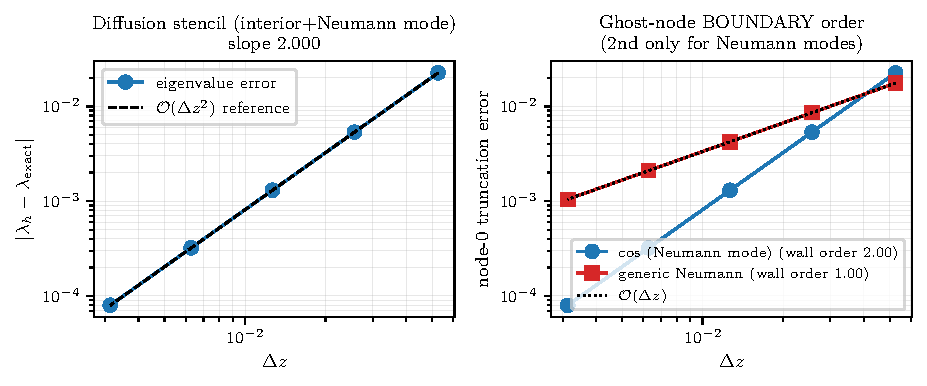
\includegraphics[width=0.72\linewidth]{pde_verify_convergence.pdf}
  \caption[Diffusion-stencil convergence and boundary order]{Grid refinement of the diffusion
  stencil (reaction off, closed box). \textbf{Left:} error of the operator eigenvalue closest
  to the analytic $-D(\pi/L)^2$ Neumann mode; least-squares slope $2.00$ confirms
  $\mathcal{O}(\Delta z^2)$ interior accuracy. \textbf{Right:} node-$0$ truncation
  error at the ghost-node wall --- $\mathcal{O}(\Delta z)$ for a generic Neumann function.}
  \label{fig:pde_convergence}
\end{figure}

\begin{figure}[htbp]
  \centering
  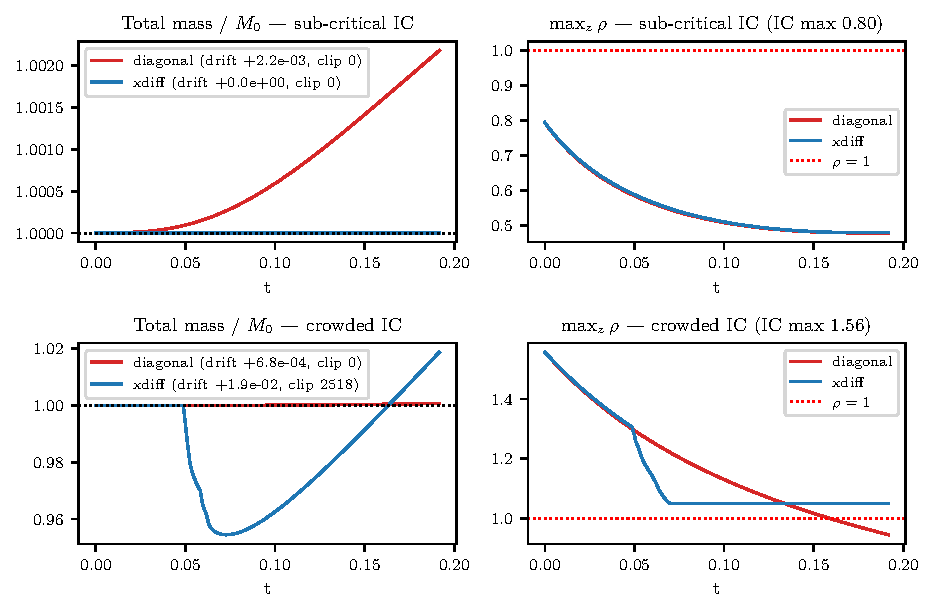
\includegraphics[width=0.72\linewidth]{pde_verify_conservation.pdf}
  \caption[Mass conservation: diagonal vs.\ volume-filling cross-diffusion]{Closed-box
  conservation, diagonal (red) vs.\ volume-filling cross-diffusion (blue).
  \textbf{Top} (sub-critical, $\rho_{\max}\!\approx\!0.80$): diagonal drifts $+2.18\times10^{-3}$;
  cross-diffusion conserves to machine precision.
  \textbf{Bottom} (crowded, $\rho_{\max}\!=\!1.56$): diagonal clips exceed unity; cross-diffusion
  degeneracy caps $\rho$ near one.}
  \label{fig:pde_conservation}
\end{figure}

\begin{table}[htbp]
  \centering
  \caption[PDE transport verification results]{Measured verification outcomes
  (\texttt{verify\_pde\_numerics.py}, reaction off, closed box).}
  \label{tab:pde_verify}
  \small
  \begin{tabular}{llccc}
    \toprule
    Test & Scheme & Mass drift & $\rho_{\max}$ & Clip \\
    \midrule
    Convergence ($N_z\!=\!20$--$320$) & diagonal interior & \multicolumn{3}{l}{slope $2.00$ ($\mathcal{O}(\Delta z^2)$)}\\
    Boundary order (generic mode)     & ghost-node wall   & \multicolumn{3}{l}{slope $1.00$ ($\mathcal{O}(\Delta z)$)}\\
    \addlinespace
    Conservation, sub-critical & diagonal        & $+2.18\times10^{-3}$ & $0.79$ & $0$ \\
    Conservation, sub-critical & cross-diffusion & $0.0$ (mach.\ prec.) & $0.79$ & $0$ \\
    Conservation, crowded      & diagonal        & $+6.8\times10^{-4}$ & $1.56$ & $0$ \\
    Conservation, crowded      & cross-diffusion & $+1.9\times10^{-2}$ & $1.56$ & $2518$ \\
    \bottomrule
  \end{tabular}
\end{table}

\section*{FISH channel decode}

\begin{figure}[htbp]
  \centering
  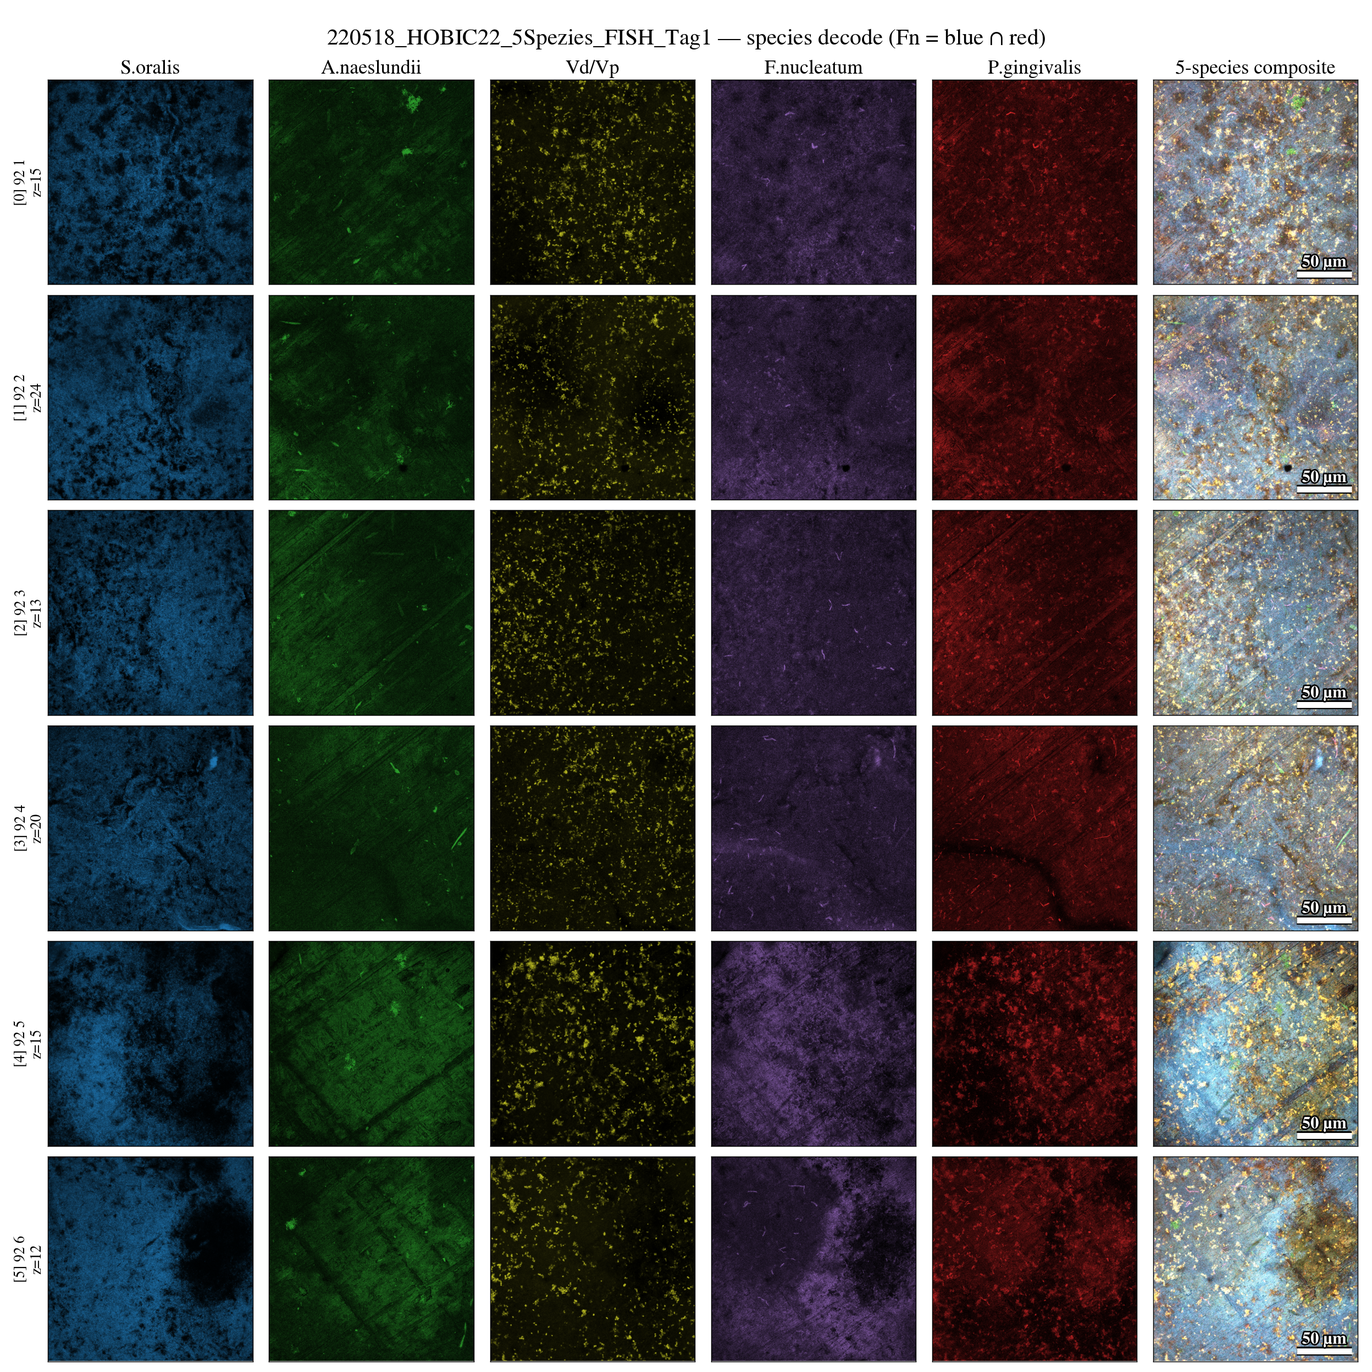
\includegraphics[width=0.85\linewidth]{fig_fish_species_decode.png}
  \caption[HOBIC FISH: 5-species channel decode]{%
  Representative HOBIC FISH acquisition (commensal-HOBIC, Day~1, titanium substrate).
  Each column shows the confocal channel for one species
  (\textit{S.~oralis}, \textit{A.~naeslundii}, \textit{Vd/Vp},
  \textit{F.~nucleatum}, \textit{P.~gingivalis}) and the five-species composite
  (right); rows are independent fields of view.
  \textit{F.~nucleatum} is decoded from the blue $\cap$ red double-label channel.
  Scale bar: $50\,\mu\mathrm{m}$.}
  \label{fig:fish_species_decode}
\end{figure}

The species diffusivities $D_i$ are being calibrated against the CLSM $z$-profiles by a
grid/regularisation sweep on the cluster; the commensal-HOBIC fit has converged
(loss $\approx0.015$) while the dysbiotic-HOBIC fit is still in progress.

\chapter{In-Vivo Analysis: Supplementary Figures}
\label{app:dieckow_supp}

\begin{figure}[htbp]
  \centering
  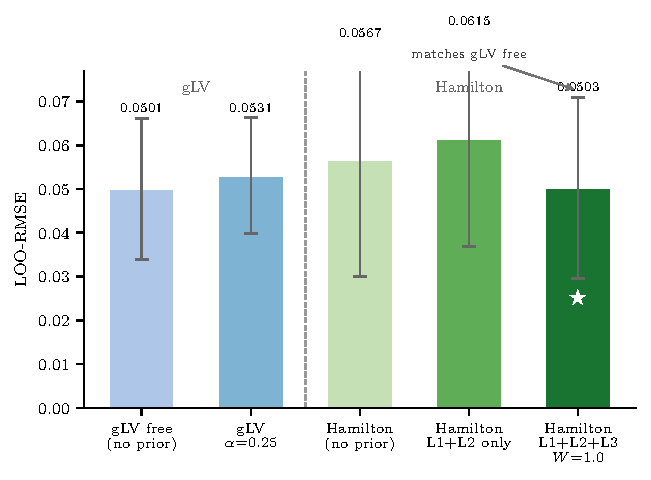
\includegraphics[width=0.74\textwidth]{fig_loo_rmse_comparison.pdf}
  \caption[LOO-RMSE comparison across model variants]{LOO-RMSE ($\text{mean}\pm\text{std}$
  across 10 folds) for gLV and Hamilton variants. The Hamilton model with the full
  three-layer prior ($W{=}1.0$, $\bigstar$) matches the gLV free baseline ($0.0503$
  vs.\ $0.0501$) despite imposing $35$ metabolic sign constraints --- sign
  regularisation recovers predictive accuracy at no cost.}
  \label{fig:loo_rmse_comparison}
\end{figure}

\begin{figure}[htbp]
  \centering
  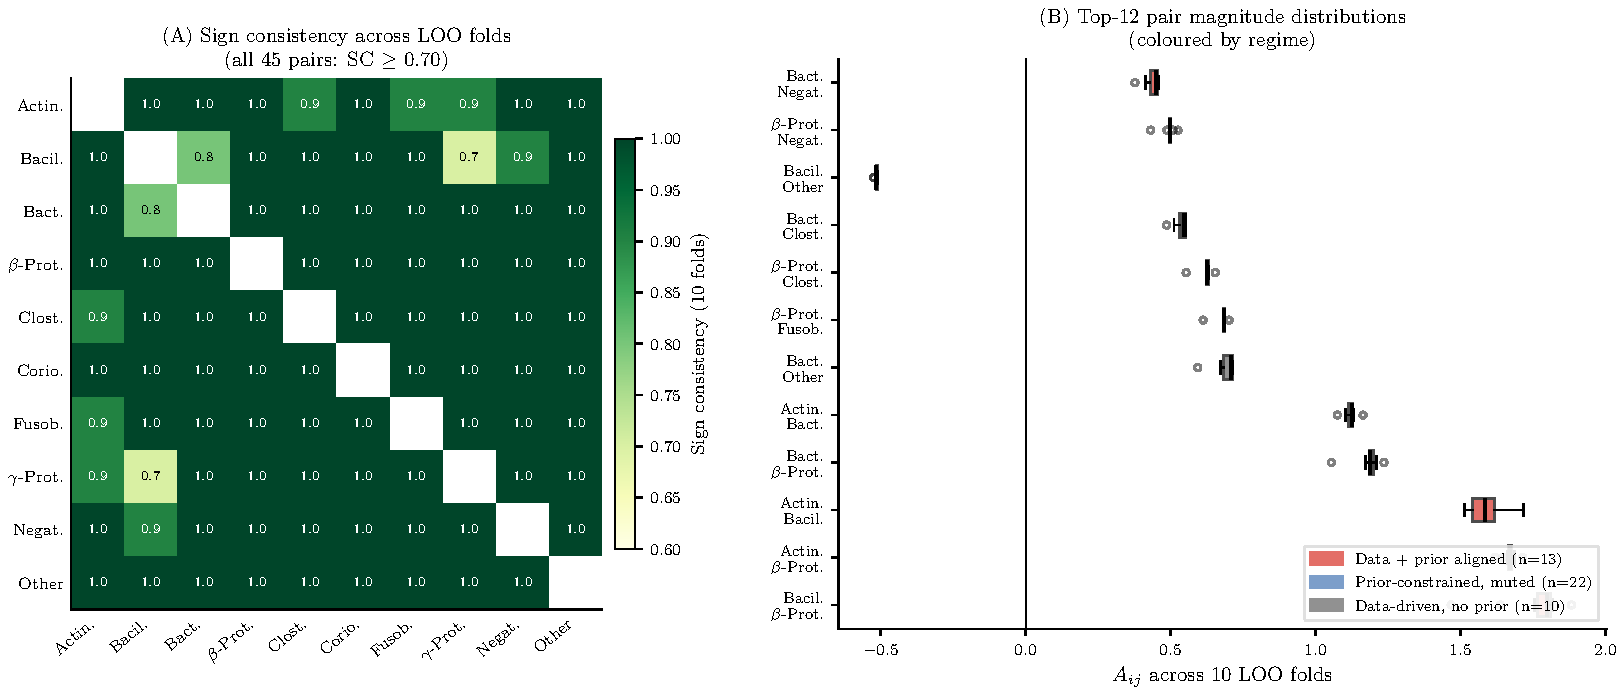
\includegraphics[width=0.70\textwidth]{dieckow_stability.pdf}
  \caption[LOO stability of the interaction matrix]{LOO stability (gLV
  $\alpha{=}0.25$, $10$ folds). \textbf{(A)} sign-consistency heatmap (boxed cells
  carry a sign constraint): $31/45$ at SC$=1.00$, $40/45$ at SC$\geq0.90$.
  \textbf{(B)} $|\bar A_{ij}|$ vs.\ fold-to-fold std by regime. \textbf{(C)}
  distributions of the strongest pairs.}
  \label{fig:dieckow_stability}
\end{figure}

\begin{figure}[htbp]
  \centering
  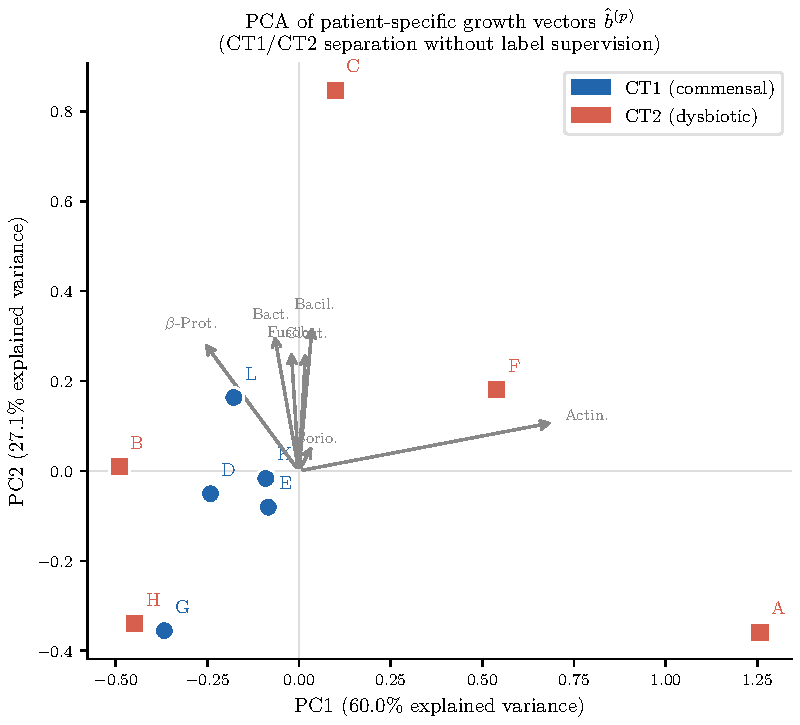
\includegraphics[width=0.62\textwidth]{dieckow_b_pca.pdf}
  \caption[Growth-vector clustering by community type]{PCA of patient growth
  vectors $\hat\bb^{(p)}$. PC1 separates CT1 (triangles) from CT2 (circles) with no
  label supervision --- patient-level ecology lives in $\bb$, not in the shared
  $\bA$.}
  \label{fig:dieckow_bpca}
\end{figure}


% ── Declaration ──────────────────────────────────────────────────────────────
\chapter*{Acknowledgements}
\addcontentsline{toc}{chapter}{Acknowledgements}
% DRAFT — finalise wording (and funding statement) before submission.
I thank my supervisor, Prof.\ Dr.-Ing.\ habil.\ Philipp Junker (Institut für
Kontinuumsmechanik, IKM), for his guidance and for the continuum-mechanical
foundation on which this work builds, and Dr.\ Meisam Soleimani for his advice on
the numerical methods. I am grateful to Felix Klempt and Hendrik Geisler for many
discussions on the Hamilton biofilm model and its implementation.

This work was carried out in collaboration with the Hannover Medical School (MHH)
and the Lower Saxony Centre for Biomedical Engineering, Implant Research and
Development (NIFE). I thank Dr.\ Szymon~P.\ Szafra\'{n}ski for hosting and guiding
the NIFE research internship and for the metabolic and microbiological insight that
shaped the in-vivo work, and Nils Heine, Dr.\ Katharina Doll-Nikutta,
Dr.\ Rumjhum Mukherjee, and Prof.\ Meike Stiesch for the experimental data and their
biological interpretation.

I also thank Assoc.\ Prof.\ Mayu Muramatsu (Keio University) for her encouragement
and for discussions on continuing this line of work toward computational solid
mechanics.

I gratefully acknowledge financial support from the JASSO (Japan Student Services
Organization) Student Exchange Support Program (Scholarship for Short-Term Study
Abroad) and the Yoshiaki Ishii Human Resource Development Scholarship of Keio
University, which together supported this double-degree research stay in Hannover.
% TODO: confirm before asserting any specific grant (see MONTHLY_EMAIL_STRATEGY).
% This research was conducted within the SFB/TRR-298 SIIRI consortium [confirm].

Finally, I thank my family and friends for their support throughout this work.

\newpage
\chapter*{Selbstständigkeitserklärung}
\addcontentsline{toc}{chapter}{Selbstständigkeitserklärung}

Hiermit erkläre ich, dass ich die vorliegende Masterarbeit selbstständig verfasst
und keine anderen als die angegebenen Hilfsmittel verwendet habe.
Alle Stellen, die wörtlich oder sinngemäß aus anderen Werken übernommen wurden,
sind als solche kenntlich gemacht.
Diese Arbeit wurde in gleicher oder ähnlicher Form noch keiner anderen
Prüfungsbehörde vorgelegt.

\vspace{2cm}
\noindent
Hannover, \underline{\hspace{4cm}} \hfill
Unterschrift: \underline{\hspace{5cm}}

\end{document}
